%%%%%%%%%%%%%%%%%%%%%%%%%%%%%%%%%%%%%%%%%%%%%%%%%%%%%%%%%%%%%%%%%%%%%%%%%%%
% Trim Size : 11in x 8.5in
% Text Area : 9.6in (include Runningheads) x 7in
% ws-ijbc.tex, 24 Jan 2010
% Tex file to use with ws-ijbc.cls written in Latex2E.
% The content, structure, format and layout of this style file is the
% property of World Scientific Publishing Co. Pte. Ltd.
%%%%%%%%%%%%%%%%%%%%%%%%%%%%%%%%%%%%%%%%%%%%%%%%%%%%%%%%%%%%%%%%%%%%%%%%%%%
%

%\documentclass[•]{•}ass[draft]{ws-ijbc}
\documentclass{ws-ijbc}
\usepackage{ws-rotating}     % used only when sideways tables/figures are used
\usepackage{epstopdf}
\usepackage{mathrsfs}
\usepackage{graphicx}
\usepackage{float}
\usepackage{bm}
\newcommand{\norm}[1]{\left\lVert#1\right\rVert}

\makeatletter
\newcommand*{\getlength}[1]{\strip@pt\dimexpr0.035136\dimexpr#1\relax\relax}
\newcommand{\showfont}{%
encoding: \f@encoding{},\\
family: \f@family{},\\
series: \f@series{},\\
shape: \f@shape{},\\
size: \f@size{} pt,\\
text height: \getlength{\the\textheight} cm,\\
text width:     \getlength{\the\textwidth} cm}
\makeatother

\usepackage{color}
\newcommand{\eHMO}[1]{\textcolor{blue}{\textbf{#1}}}

\begin{document}

\catchline{}{}{}{}{} % Publisher's Area please ignore

\markboth{Elle Musoke, Bernd Krauskopf and Hinke M. Osinga}{Heteroclinic connections between two saddle slow manifolds in the Olsen model}

\title{A surface of heteroclinic connections between \\ two saddle slow manifolds in the Olsen model}

\author{Elle Musoke, Bernd Krauskopf and Hinke M. Osinga}


\address{Department of Mathematics, University of Auckland \\
  Private Bag 92019, Auckland 1142, New Zealand \\
elle.musoke@auckland.ac.nz; b.krauskopf@auckland.ac.nz; h.m.osinga@auckland.ac.nz}

\maketitle

\begin{history}
\received{(to be inserted by publisher)}
\end{history}

%%%%%%%%%%%%%%%%%%%%%%%%%%%%%%%%%%%%%%%%%%%%%%%%%%%%%%%%%%
\begin{abstract}
  The Olsen model for the biochemical peroxidase-oxidase reaction has a parameter regime where one of its four variables evolves much slower than the other three. It is characterized by the existence of periodic orbits along which a large oscillation is followed by many much smaller oscillations before the process repeats. We are concerned here with a crucial ingredient for such mixed-mode oscillations (MMOs) in the Olsen model: a surface of connecting orbits that is followed closely by the MMO periodic orbit during its global, large-amplitude transition back to another onset of small oscillations. Importantly, orbits on this surface connect two one-dimensional saddle slow manifolds, which exist near the curve of equilibria of the limit where the slow variable is frozen and acts as a parameter of the so-called fast subsystem. 

\hspace*{7mm}We present a numerical method, based on formulating suitable boundary value problems, to compute such a surface of connecting orbits. It involves a number of steps to compute the slow manifolds, certain submanifolds of their stable and unstable manifolds and, finally, a first connecting orbit that is then used to sweep out the surface by continuation. If it exists, such a surface of connecting orbits between two one-dimensional saddle slow manifolds is robust under parameter variations. We compute and visualize it in the Olsen model and show how this surface organizes the global return mechanism of MMO periodic orbits from the end of small oscillations back to a region of phase space where they start again. 
\end{abstract}
%%%%%%%%%%%%%%%%%%%%%%%%%%%%%%%%%%%%%%%%%%%%%%%%%%%%%%%%%%

\keywords{Geometric singular perturbation theory; slow manifold; heteroclinic orbit; mixed-mode oscillation, boundary value problem formulation, Lin's method.}


%%%%%%%%%%%%%%%%%%%%%%%%%%%%%%%%%%%%%%%%%%%%%%%%%%%%%%%%%%
\section{Introduction}
%
Olsen~[1983] derived a system of four differential equations that describes the biochemical reaction that oxidises the substrate nicotinamide adenine dinucleotide (NADH) with the enzyme peroxidase as the catalyst. There is no universally agreed mathematical model for this peroxidase-oxidase reaction, but the reaction chain involves at least two intermediate free radicals, which means that the model is at least four dimensional. Olsen showed that a four-dimensional system, referred to as the Olsen model and introduced in detail below, is indeed sufficient to produce experimentally observed phenomena, including complicated oscillations, bistability, and chaotic behavior~\cite{Olsen}. The Olsen model is of particular interest to mathematicians because the periodic oscillations are of so-called mixed-mode type: localized small-amplitude oscillations (SAOs) are combined with global large-amplitude oscillations (LAOs) into a complicated periodic pattern. Mixed-mode oscillations (MMOs) are known to occur in chemical reactions~\cite{BZ, BZ_reaction}, but they are also ubiquitous, for example, in neuronal spiking patterns and lasers; see~\cite{MMO} and references therein. The Olsen model can exhibit different types of MMOs, including some with several LAOs before a phase of SAOs, and this has also been observed experimentally~\cite{Olsen}.

From a mathematical point of view, dynamical systems that exhibit MMOs are generally characterized by a difference in time scales, or evolution rates, of the different system variables. In its simplest form, such a time-scale separation is global in the sense that the variables are divided into different groups that evolve on different time scales, which is represented by one or more time-scale separation parameters that multiply respective groups of variables. However, in many models, and this is also the case for the Olsen model, there is no such global time scale separation; rather the time scales of the variables depend on the choice of intrinsic system parameters and on what regions of phase space are visited by a trajectory of interest, such as an MMO periodic orbit.
We study the Olsen model in the parameter regime considered in~\cite{QSSA}, where it features stable periodic MMOs with a single LAO followed by many SAOs. While it nominally has three different time-scales, the Olsen model has one slow and three fast variables for this choice of parameters~\cite{Rescaling}. 

Slow-fast systems with a single time-scale separation $\varepsilon$ can be studied with the tools of geometric singular perturbation theory (GSPT) \cite{Jones} as introduced by \cite{Fenichel}. The main result is that invariant objects of the limiting (lower-dimensional) slow and fast subsystems for $\varepsilon = 0$ give rise to nearby corresponding `slow objects' that organise the slow-fast dynamics. Key in this context are the objects on which the slow flow lives: equilibria of the fast subsystem, formed by the intersection of the nullclines associated with the fast variables, define the so-called critical manifold that perturbs to (branches of) the slow manifold for $\varepsilon > 0$. When there is a single slow variable, as for the Olsen model we study here, the critical manifold and the associated branches of slow manifolds are curves in phase space. Moreover, the critical manifold we encounter in the Olsen model is cubic or S-shaped with branches that meet at fold points with respect to the slow variable. 

The existence of an S-shaped critical manifold is a robust phenomenon whose relevance goes all the way back to the study of planar slow-fast systems, notably the famous Van der Pol oscillator~\cite{vdpol} and FitzHugh--Nagumo  model~\cite{FH,Nagumo}. Their well-known relaxation oscillations track an attracting branch towards the fold of the critical manifold, then make a fast transition to the other attracting branch, where the slow flow is in the opposite direction; the trajectory then approaches the other fold, where it makes a fast transition back, and the process repeats. The two attracting branches are connected by a repelling branch of the critical manifold. As it turned out, this repelling branch may be followed closely by certain periodic orbits, which are referred to as canard cycles \cite{canard_explosion}. They were found in an exponentially small range of a system parameter, where small periodic orbits born in a Hopf bifurcation exhibit a sudden, rapid increase in amplitude to become large relaxation oscillations. This phenomenon is known as a canard explosion; see, for example, \cite{MMO, GH} for more details on these now classical results.

S-shaped one-dimensional critical manifolds also play an important part for understanding the slow-fast dynamics of mathematical models with a phase space of dimension three, meaning that there are now two fast variables in addition to the slow variable.\footnote{Three-dimensional slow-fast systems with one fast and two slow variables are beyond the scope of this paper but also very interesting. They provide robust mechanisms for the generation of different types of MMOs organized by what are known as folded singularities, which generate transverse intersections of attracting and repelling slow manifolds in structurally stable canard orbits; see, for example, \cite{lents-rapides, SW} and \cite{MMO} as an entry point to the literature.} In particular, S-shaped critical manifolds can be found as a main ingredient in neuron models of Hodgkin--Huxley type~\cite{HH} that show bursting behavior characterized by periods of high-frequency spiking and quiescent periods in between. Rinzel~[1987] successfully applied GSPT to explain different types of bursting patters of neurons in terms of the bifurcation structure of the fast subsystem. The ideas of Rinzel led to the discovery and classification of many different bursting patterns, many of which have been collected in~\cite{izh00}. The critical manifold in these types of models is often an S-shaped curve that contains equilibria of all stability types; see~\cite{rinzel87}. In other words, compared to the planar case, there are now new possibilities for the dynamics associated with an S-shaped critical manifold. First of all, when an attracting (stable) branch of the critical manifold loses stability at a fold point, the accompanying branch is now of saddle type, consisting of equilibria of the fast subsystem with one repelling and otherwise attracting directions. Moreover, stability along a branch of the critical manifold can now change not only fold points (as for the planar case) but also at Hopf bifurcations of the fast subsystem (which requires at least two fast variables). Finally, a Hopf bifurcation generates a family of bifurcating periodic orbits of the fast subsystem, which may be stable or unstable, change stability at fold (or saddle-node) bifurcations, and may or may not grow to reach a point on a saddle branch of the S-shaped critical manifolds to form a homoclinic orbit. The different possibilities create quite a large number of different cases that are at the core of the classification of bursting neurons \cite{izh00,rinzel87}.

Two bursting patterns, known as square-wave (fold/homoclinic) bursting and pseudo-plateau bursting, show the specific characteristics of an MMO, namely, lots of SAOs followed by a single LAO. Both are quite closely related \cite{osta-dcds} and can be generated with a three-dimensional system that has one slow variable and an S-shaped critical manifold. More specifically, an attracting branch of the critical manifold becomes repelling at a Hopf bifurcation; the repelling branch connects at a fold point to a saddle branch that connects to a different attracting branch at a second fold point. For square-wave bursting, the Hopf bifurcation is supercritical and for pseudo-plateau bursting it is subcritical, but for both cases the emanating family of periodic orbits ends at a homoclinic bifurcation where the family reaches a saddle equilibrium on the middle branch. In the context of bursting in the full three-dimensional system, the family of (respectively attracting and repelling) periodic orbits gives rise to fast oscillations along a slow segment of the MMO; see also~\cite{bertram95, osta-dcds, sols-bmb}. In both cases, one LAO brings trajectories back to the SAO regime because of the S-shaped nature of the critical manifold, generating a periodic MMO.\footnote{In general, MMOs tend to be associated with slow-fast systems that have two slow variables~\cite{vdp2, MMO, vdp1, Autocatalator, SW, Wech2005}; in fact, pseudo-plateau bursting has also been classified as an MMO generated by a system with two slow variables~\cite{Vo_paper}.}

There are even more possibilities for the dynamics associated with a one-dimensional S-shaped critical manifold in a system of dimension four. In particular, a fold point may now connect two saddle branches of the slow manifold, and this is exactly the situation we encounter in the Olsen model. More specifically, in the parameter regime we consider, the S-shaped critical manifold for $\varepsilon = 0$ of the Olsen model is essentially that of the pseudo-plateau burster but, importantly, there are now three fast variables. Therefore, and in contrast to three-dimensional slow-fast systems with a single slow variable, the equilibria on the critical manifold `past' the Hopf bifurcation are not repelling, but they are saddles with two unstable and one stable eigenvalues. On the other hand, the saddle equilibria in between the fold points on the S-shaped critical manifold have only one unstable, but two stable eigenvalues. Indeed, in three dimensions, such a difference in saddle index is not possible. 

As we will show is the case for the Olsen model, this configuration of an S-shaped critical manifold in four dimensions may generate a surface of heteroclinic connecting orbits between the two associated saddle branches of the slow manifold for nonzero $\varepsilon$. This situation is robust, because the two saddle branches of the critical manifold have a three-dimensional stable and a three-dimensional unstable manifold, respectively, which perturb to stable and unstable manifolds of the two slow manifolds with the same dimensions~\cite{Fenichel}. Two three-dimensional manifolds in a four-dimensional phase space are generically expected to intersect and, if they do, they intersect robustly in a two-dimensional surface of heteroclinic solutions. More technically, slow manifolds for nonzero $\varepsilon$ are defined by the property that they stay $O(\varepsilon)$ close to the respective branch of the critical manifold for a time of $O(1)$~\cite{gk-siads09, Saeed_Paper}. Similarly, their stable and unstable manifolds can be viewed as solution families that contain orbit segments that rapidly converge to a saddle slow manifold and then remain $O(\varepsilon)$ close to it for $O(1)$ time~\cite{gk-siads09, Cris_paper, Saeed_Paper}. 

The challenge that we address in this paper is to develop a numerical method capable of finding the surface of heteroclinic connections between two slow manifolds. We achieve this by defining suitable families of orbit segments, which are then found as solutions of corresponding well-posed boundary value problems (BVPs). This BVP approach is accurate and flexible; it can be used for computing various invariant objects of a given dynamical system~\cite{Red_book}. In particular, it is well suited to the context of slow-fast systems, where it has been employed to compute attracting and repelling slow manifolds of dimensions one and two; see ~\cite{MMO,Cris_paper,homotopy_example}. Saddle slow manifolds, on the other hand, tend to be approximated by a saddle segment of the critical manifold, which is then used to compute approximate stable or unstable manifolds of the saddle slow manifold~\cite{QSSA, gk-siads09, Cris_paper}; see also~\cite{Emily_Harvey_paper, nota-jmn}. More recently, a method was presented in~\cite{Saeed_Paper} that computes the saddle slow manifold of a three-dimensional system; the underlying idea is to find (a suitably large part of) the saddle slow manifold with a BVP set-up to find an orbit that starts in its stable manifold, follows the slow manifold for $O(1)$ time and then leaves it along its unstable manifold. The local two-dimensional stable and unstable manifolds found as part of this set-up can then be extended into parts of phase space beyond a neighborhood of the slow manifold; see~\cite{Saeed_Paper} where the stable manifold was shown to organize spike adding in a parameter-dependent model of pseudo-plateau bursting.

We present here a method for computing a surface of heteroclinic connections between two saddle slow manifolds. More specifically, this is achieved in several steps, each with a dedicated BVP set-up whose solutions are found with the boundary value problem solver of the continuation package \textsc{AUTO}~\cite{autoOriginal, auto}. First of all, we extend the approach from~\cite{Saeed_Paper} to systems with three fast variables to find the two saddle slow manifolds of different index (number of unstable directions). Subsequently, we set up a BVP formulation that allows us to compute suitable two-dimensional submanifolds of their respective three-dimensional stable and unstable manifolds; this is similar in spirit to the approach taken in~\cite{Cris_paper}.

The crucial part of our method is to find a first heteroclinic connection, that is, an orbit that lies in the stable manifold of one slow manifold as well as the unstable manifold of the other slow manifold. We determine such a heteroclinic orbit in a systematic way with a novel implementation of Lin's method~\cite{Lin_original, Lin_POs, Lin_POs2}. In a nutshell, we consider a BVP set-up for two orbit segments, the first in the stable manifold and the other in the unstable manifold of the respective slow manifolds, such that both orbit segments have an end point in a common three-dimensional section; these two orbit segments are coupled by requiring that their end points in the section lie along a fixed direction, called the Lin direction. A heteroclinic orbit can then be found as a zero of the the (signed) distance in the Lin direction; see Section~\ref{sec:hetconn} for details. This heteroclinc orbit is then used to sweep out the surface of heteroclinic connections by continuation. We present and illustrate the necessary BVP formulations one-by-one for the Olsen model. While there are certain specific choices that we make for this particular system, our set-up for finding the surface of heteroclinic connections is general and can be applied to any slow-fast system with a one-dimensional critical manifold that has two saddle branches of different index.

Our computations for the Olsen model show that there is indeed a surface of connecting orbits between two saddle slow manifolds. The existence of such a surface was already suggested in~\cite{QSSA}, which was based on a model reduction, and this is confirmed by our calculations. Indeed, the Olsen model provides the first example of such a surface of connecting orbits, whose existence is a robust property. Our direct computation of this surface in the full four-dimensional phase space allows us to study its properties and the role it plays in the dynamics behind the MMOs of the Olsen model. To this end, we render the surface in different three-dimensional projections, compare it with its singular limit, which we also ompute with a Lin's method approach, and show it together with the stable MMO periodic orbit. This shows that the surface of connecting orbits plays a crucial part in the global reinjection mechanism of the MMO. An LAO is formed when the trajectory exits a region of SAOs near one saddle branch of the slow manifold by traveling via the surface of heteroclinic connections to the other saddle branch of the slow manifold, before a fast transition back to the region of SAOs. We also follow the MMO periodic orbit towards smaller values of the time-scale separation parameter $\varepsilon$ and find that it lies on an isola that does not reach the singular limit $\varepsilon = 0$. As we show, when the parameter $\varepsilon$ moves around the isola, the MMO changes quite dramatically but the the surface of heteroclinic connections continues to play a part in the reinjection mechanism.  

This paper is organized as follows. The next section presents the Olsen model as studied here and introduces the necessary notions from GPST, including the saddle slow manifolds and their stable and unstable manifolds.  In Section~\ref{sec:slowmans} we present practical definitions of these manifolds, which then are translated to a respective BVP set-up used to compute them; this is done in Section~\ref{sec:S3} for slow manifolds themselves, in Section~\ref{sec:compWsS3}  for the respective three-dimensional stable manifold of the one, and in Section~\ref{sec:compWuS2} for the respective three-dimensional unstable manifold of the other saddle slow manifold. Section~\ref{sec:hetconn} introduces the Lin's method set-up that allows us to compute the surface of heteroclinic connections between two branches of the slow manifold, and Section~\ref{sec:hetconn0} presents the set-up for finding its singular limit, that is, the surface of heteroclinic connections between the corresponding two saddle branches of the critical manifold. Section~\ref{sec:mmogeom} then discusses and illustrates the role this surface has for the organization of the (stable) MMO in the Olsen model, as well as for all MMO periodic orbits along an isola that is found by continuation of the MMO in the time-scale parameter $\varepsilon$. Conclusions and an outlook are given in Section~\ref{sec:concl}. Finally, the Appendix provides details of how we compute an estimate of the distance between the surface of connections and its singular limit.


%%%%%%%%%%%%%%%%%%%%%%%%%%%%%%%%%%%%%%%%%%%%%%%%%%%%%%%%%%
\section{The Olsen Model}
\label{sec:olsen}
%
%%%%%%%%%%%%%%%%%%%%%%%%%%%%%%%%%%%%%%%%%%%%%%%%%%%%%%%%%%
\begin{table}[t!]
\tbl{Parameters of system \eqref{equation_1} as in \cite{Rescaling} so that $A$, $X$, and $Y$ are fast and $B$ is slow.}
{\begin{tabular}{c  c  c  c  c  c  c  c  c} \\[-2pt]
\toprule
$\alpha$ & $\delta$ & $\varepsilon$ & $\lambda$ & $\kappa$ & $\mu$ & $\zeta$ \\[6pt]
\hline\\[-6pt]
0.0912 & $1.2121 \times 10^{-5}$ & 0.0037 & 18.5281 & 3.7963 & 0.9697 & 0.9847\\[1pt]
\botrule
\end{tabular}}
\label{table:pars}
\end{table}
%%%%%%%%%%%%%%%%%%%%%%%%%%%%%%%%%%%%%%%%%%%%%%%%%%%%%%%%%%
 
We consider the prototypical four-dimensional Olsen model for peroxidase-oxidase reaction \cite{Olsen} in its scaled form from \cite{Rescaling}, given as the system of ordinary differential equations
%
\begin{equation}
\begin{aligned}
\begin{cases}
\frac{dA}{dt} &= \mu - \alpha A - ABY, \\[1mm]
\frac{dB}{dt} &= \varepsilon(1-BX - ABY), \\[1mm]
\frac{dX}{dt} &= \lambda(BX - X^2 +3ABY - \zeta X + \delta), \\[1mm]
\frac{dY}{dt} &= \kappa\lambda(X^2 - Y - ABY),
\end{cases}
\end{aligned}
\label{equation_1}
\end{equation}
%
where $(A, B, X, Y)\in\mathbb{R}^{4}$ are positive concentrations of chemicals.  The system parameters are represented by Greek letters that have the values given in Table~\ref{table:pars}.  These are the same values as in \cite{Rescaling}, with the minor modification of using $\varepsilon$ for $\varepsilon_{b}$ and $\frac{1}{\lambda}$ for $\varepsilon^{2}$ for notational convenience.  The time-scaling parameters $\varepsilon$ and $\lambda$ are chosen so that we may consider $A$, $X$, and $Y$ as fast variables, and $B$ as a slow variable; see \cite{Rescaling}.

The classical analysis of slow-fast systems considers two singular limits for systems with two time-scales; for example, see \cite{MMO}.  In the limit of $\varepsilon = 0$, system \eqref{equation_1} reduces to
%
\begin{equation}
\begin{aligned}
\begin{cases}
\frac{dA}{dt} &= \mu - \alpha A - ABY, \\[1mm]
\frac{dX}{dt} &= \lambda(BX - X^2 +3ABY - \zeta X + \delta), \\[1mm]
\frac{dY}{dt} &= \kappa \lambda(X^2 - Y - ABY),
\end{cases}
\end{aligned}
\label{equation_2}
\end{equation}
%
with $\frac{dB}{dt}=0$, meaning that $B$ is a parameter of \eqref{equation_2}.  We refer to the three-dimensional system \eqref{equation_2} as the fast subsystem.  Performing the time rescaling $\tau = \varepsilon t$ and then considering the limit of $\varepsilon = 0$, system \eqref{equation_1} reduces to the differential algebraic system
%    
\begin{equation}
\begin{aligned}
\begin{cases}
0 &= \mu - \alpha A - ABY, \\[1mm]
\frac{dB}{d\tau} &= (1-BX - ABY), \\[1mm]
0 &= \lambda (BX - X^2 +3ABY - \zeta X + \delta), \\[1mm]
0 &= \kappa \lambda(X^2 - Y - ABY).
\end{cases}
\end{aligned}
\label{equation_3}
\end{equation}
%
The three algebraic equations in system \eqref{equation_3} define a one-dimensional manifold, called the critical manifold, denoted $C$.

The critical manifold $C$ consists of equilibria of the fast subsystem \eqref{equation_2}, which exist in $(A,B,X,Y)$-space.  Their stability can be determined from the eigenvalues of the $3\times3$ Jacobian matrix of \eqref{equation_2} evaluated at each point on the critical manifold for the appropriate value of $B$.  Points $p \in C$ at which the Jacobian of \eqref{equation_2} has eigenvalues with non-zero real parts are called hyperbolic.  Eigenvectors whose associated eigenvalues have negative real parts are called stable directions of $p$ and these span the stable eigenspace $E^{s}(p)$ of $p$.  The unstable directions and the unstable eigenspace $E^{u}(p)$ are defined similarly by the eigenvectors associated with eigenvalues having positive real part.  Note that the dimensions of the stable and unstable eigenspaces are equal to the number of eigenvalues with negative and positive real parts, respectively.  Equilibria at which the Jacobian has eigenvalues with zero real part are called non-hyperbolic and these correspond to bifurcations of system \eqref{equation_2} \cite{The_Kuz} .

The critical manifold $C$ in $(A,B,X,Y)$-space is divided into branches by bifurcation points of the fast subsystem \eqref{equation_2}, so that points on each branch have the same dimensions of stable and unstable eigenspaces.  In other words, the branches of $C$ are one-parameter families in $B$ of hyperbolic equilibria of system \eqref{equation_2}.  We define the stable eigenspace $E^s(C^i)$ of a branch $C^i$ as the collection of stable eigenspaces of all the points on the branch.  Hence, the dimension of $E^s(C^i)$ is one higher than the dimension of the stable eigenspace of each point on the branch. 

%%%%%%%%%%%%%%%%%%%%%%%%%%%%%%%%%%%%%%%%%%%%%%%%%%%%%%%%%%
\begin{figure}[!t]
\centering
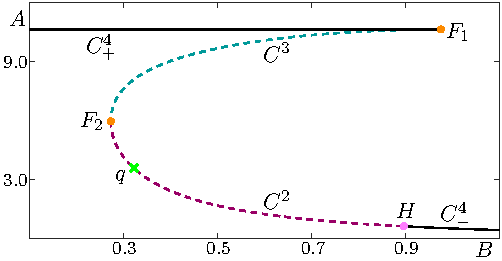
\includegraphics[]{./figures/MKMO_1.pdf}
\caption{Physically relevant branches $C^2$, $C^3$, $C^4_\pm$ of the critical manifold of \eqref{equation_1} shown in projection onto the $(B,A)$-plane.  Branches $C^2$ (dashed, raspberry curve) and $C^3$ (dashed, teal curve) consist of saddles of \eqref{equation_2} and $C^4_\pm$ (solid, black curve) consist of attractors of \eqref{equation_2}.  Superscripts indicate the dimension of the stable eigenspace of the branch and subscripts are used to distinguish between the two branches of attractors.  Branches are divided by saddle-node bifurcation points $F_1$ and $F_2$ (orange dots) and a Hopf point $H$ (pink dot).  Also shown is the saddle equilibrium $q$ (green cross) of \eqref{equation_1} on $C^2$.}
\label{figure_1}
\end{figure}
%%%%%%%%%%%%%%%%%%%%%%%%%%%%%%%%%%%%%%%%%%%%%%%%%%%%%%%%%%

Four branches of $C$ lie in the physically relevant region where all phase-space variables are positive, and two of these are attracting.  The four branches are shown in Figure~\ref{figure_1} in projection onto the $(B,A)$-plane.  In our notation for branches, superscripts indicate the dimension in $(A,B,X,Y)$-space of the stable eigenspace of the branch.  Further, we use subscripts to distinguish the two branches on which equilibria have three-dimensional stable eigenspaces, that is, are attracting.   The uppermost branch, denoted $C^4_+$ (solid, black curve), consists of stable equilibria of \eqref{equation_2}.  It is separated from the branch of saddle equilibria, denoted $C^3$ (dashed, teal curve), by a very sharp fold at the point $F_1$ (orange dot) at $B \approx 0.956$.  Folds of the critical manifold correspond to saddle-node bifurcations of system \eqref{equation_2} with respect to the parameter $B$, these are points at which one of the real eigenvalues of the Jacobian changes sign.  Another fold at $B \approx 0.273$, denoted $F_2$ (orange dot), separates $C^3$ from a lower branch of saddle equilibria, denoted $C^2$ (dashed, raspberry curve).   The branch $C^2$ ends at a Hopf bifurcation $H$ (pink dot) at $B \approx 0.897$, where two complex-conjugate eigenvalues of the Jacobian pass through the imaginary axis of the complex plane.  To the right of $H$, there is again a stable branch of equilibria denoted $C^4_-$ (solid, black curve).

The point $q$ (green cross) on $C^2$ in Figure~\ref{figure_1} is an equilibrium of system \eqref{equation_3} and is, hence, an equilibrium for the full system \eqref{equation_1}.  The equilibrium $q$ has a two-dimensional stable and two-dimensional unstable manifold, denoted $W^s(q)$ and $W^u(q)$, respectively.  The manifolds $W^{s}(q)$ and $W^{u}(q)$ consist of trajectories in $(A,B,X,Y)$-space that converge to $q$ in forward and backward time respectively.  To the right of $W^u(q)$, in the $(B,A)$-projection, the flow is from right to left near $C^2$.  To the left of $W^u(q)$, in the $(B,A)$-projection, the flow is from left to right near $C^2$.  The manifolds $W^{s}(q)$ and $W^{u}(q)$ can be computed with the methods in \cite{Red_book}; they are not depicted in Figure~\ref{figure_1}, but are shown in Figure~\ref{figure_10}.

Our interest is in the branches $C^3$ and $C^2$ because they are saddle objects of different types and are crucial for organising the phase space.  These branches of the critical manifold are invariant for $\varepsilon = 0$, but not for $\varepsilon > 0$.  However, they do persist as locally invariant manifolds, called slow manifolds \cite{Fenichel}.  The associated slow manifolds are traditionally denoted $S^3_\varepsilon$ and $S^2_\varepsilon$ but, for notational convenience, we drop the subscript indicating dependence on $\varepsilon$ and refer to these slow manifolds for $\varepsilon > 0$ simply as $S^3$ and $S^2$.  The slow manifolds $S^3$ and $S^2$ have the same dimension and stability as $C^3$ and $C^2$ and lie at an $O(\varepsilon)$ Hausdorff distance from $C^3$ and $C^2$, respectively.  (For a definition of Hausdorff distance see, e.g., \cite{Hausdorff_Distance}.)  In particular, $S^3$ converges to $C^3$ as $\varepsilon \rightarrow 0$;  similarly, $S^2$ converges to $S^3$ as $\varepsilon \rightarrow 0$.  Orbit segments that lie on a slow manifold remain slow for $O(1)$ time with respect to the slow time-scale.  It follows that any trajectory that remains slow for an $O(1)$ amount of slow time can be considered (to be on) a slow manifold.  However, trajectories on a slow manifold may eventually become fast. Due to their finite-time nature, slow manifolds are not unique; however, any two slow manifolds lie exponentially close to each other in a suitable $O(\varepsilon)$ neighbourhood of the associated branch on the critical manifold \cite{Fenichel}.  We select representatives $S^3$ and $S^2$ as the slow manifolds that remain slow for the longest amount of time; see the numerical set-up in Section~\ref{sec:slowmans}.

The Stable Manifold Theorem tells us that each $p \in C^3$ has a stable and an unstable manifold that are tangent to and have the same dimensions as $E^{s}(p)$ and $E^{u}(p)$, respectively \cite{PdM, Perko_book}.  We denote the stable manifold of a point $p \in C^3$ by $W^{s}(p)$ and its unstable manifold by $W^{u}(p)$.  We can then define the collection of stable manifolds for $p \in C^3$ as $W^{s}(C^3) = \bigcup_{p \in C^3} W^{s}(p)$, which is a three-dimensional manifold tangent to $E^s(C^3)$.  We can similarly define the three-dimensional unstable manifold $W^{u}(C^2)$ of $C^2$ which is tangent to $E^u(C^2)$.

According to Fenichel Theory, for $\varepsilon > 0$, the manifold $W^{s}(C^3)$ also persists in an $O(\varepsilon)$ neighbourhood as a three-dimensional local stable manifold $W^{s}_{loc}(S^3)$ of $S^3$.  The local stable manifold $W^{s}_{loc}(S^3)$ consists of families of trajectories that have a fast approach to $S^3$ and then remain close to $S^3$ for $O(1)$ slow time.  The global stable manifold $W^{s}(S^3)$ can be obtained by extending $W^{s}_{loc}(S^3)$ backward in time.  The three-dimensional unstable manifold $W^{u}(S^2)$ associated with $S^2$ is similarly defined for backward time.  Again, due to the finite-time nature of the definitions for the three-dimensional manifolds $W^{s}(S^3)$ and $W^{u}(S^2)$, they are not unique.  To select unique representatives, we consider two-parameter families of orbit segments that remain slow for the longest amount of time, subject to boundary conditions.  In the next section, we describe our computational set-up in detail.  
 

%%%%%%%%%%%%%%%%%%%%%%%%%%%%%%%%%%%%%%%%%%%%%%%%%%%%%%%%%%
\section{Computation of saddle slow manifolds and their (un)stable manifolds}
\label{sec:slowmans}
%
In \cite{Saeed_Paper} a method is presented for the computation of a one-dimensional saddle slow manifold and its (un)stable manifolds in a three-dimensional system.  We build on this work to define and compute unique representatives $S^3$ and $S^2$ as well as their stable and unstable manifolds, respectively.

%%%%%%%%%%%%%%%%%%%%%%%%%%%%%%%%%%%%%%%%%%%%%%%%%%%%%%%%%%
\subsection{Definition of $S^3$}    
\label{sec:S3}

We define the slow manifold $S^3$ with respect to a closed interval $[B_{\mathrm{in}},B_{\mathrm{out}}]$ for the slow variable $B$.  The values for $B_{\mathrm{in}}$ and $B_{\mathrm{out}}$ are chosen such that $[B_{\mathrm{in}},B_{\mathrm{out}}] \subset (B_{F_1}, B_{F_2})$, where $B_{F_1}$ and $B_{F_2}$ are the $B$-values of the fold points $F_1$ and $F_2$, respectively.  Hence, for each $B_p \in [B_{\mathrm{in}},B_{\mathrm{out}}]$ there is a unique point $p=(p_A,p_B,p_X,p_Y) \in C^3$ such that $p_B = B_p$.  In the three-dimensional subsection $\{ \omega \in \mathbb{R}^4 \; | \; \omega_B=B_p\}$ we define a solid three-sphere $D^s_\delta(B_p)$ with radius $\delta$ and centre $p$ , given formally by
%
\begin{equation*}
D^s_\delta(B_p)=\{w \in \mathbb{R}^4 \; | \; w_B = B_p, \left\lVert w-p \right\rVert \leq \delta\}.
\end{equation*}    
\noindent
The union 
\begin{equation*}
\mathscr{D}^s = \bigcup\limits_{B_p \in [B_{\mathrm{in}}, B_{\mathrm{out}}]}^{} D^s_\delta(B_p)
\end{equation*}
%
forms a four-dimensional compact cylinder.  The superscript $s$ indicates that the radius $\delta$ is small, but it needs to be of $O(\varepsilon)$ to ensure that $S^3$ lies in $\mathscr{D}^s$.  The one-parameter family of orbit segments that enter $\mathscr{D}^s$ via $D_\delta(B_{\mathrm{in}})$ are candidates for $S^3$.   To select a representative $S^3$ we require that the orbit segment representing $S^3$ has maximal integration time in $\mathscr{D}^s$ while satisfying appropriate boundary conditions.  Our choice of boundary conditions is explained in Section~\ref{sec:compWsS3}.

%%%%%%%%%%%%%%%%%%%%%%%%%%%%%%%%%%%%%%%%%%%%%%%%%%%%%%%%%%
\begin{figure}[!t]
\begin{center}
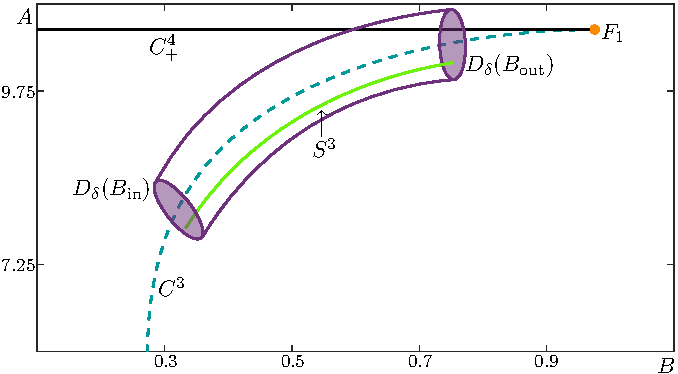
\includegraphics{./figures/MKMO_2.pdf}
\end{center}
\caption{A sketch of the selected slow manifold $S^3$ (green curve) projected onto the $(B,A)$-plane.  The slow manifold $S^3$ is defined by having the longest integration time while entering and exiting  $D^s_\delta(B_{\mathrm{in}})$ and $D^s_\delta(B_{\mathrm{out}})$ (purple disks) at either end of a four-dimensional cylinder.  Also shown are $C^3$, $C^4_+$, and $F_1$.}
\label{figure_2}
\end{figure}
%%%%%%%%%%%%%%%%%%%%%%%%%%%%%%%%%%%%%%%%%%%%%%%%%%%%%%%%%%

Figure~\ref{figure_2} illustrates this definition with an enlargement of Figure~\ref{figure_1} near the branch $C^3$, where we now sketch the relevant elements of this definition in projection onto the $(B,A)$-plane. The selected slow manifold $S^3$, enters $\mathscr{D}^s$ at $D^s_\delta(B_{\mathrm{in}})$ and exits at $D^s_\delta(B_{\mathrm{out}})$ (purple disks).


%%%%%%%%%%%%%%%%%%%%%%%%%%%%%%%%%%%%%%%%%%%%%%%%%%%%%%%%%%
\subsection{Computation of $W^{s}(S^3)$ and  $S^3$}
\label{sec:compWsS3}

Since $W^{s}(S^3)$ is three dimensional it is challenging to compute and difficult to visualise.  In fact, $W^{s}(S^3)$ can be represented as a two-parameter family of orbit segments that enter $\mathscr{D}^s$ at $D^s_{\delta}(B_p)$ for some $B_p \in [B_{\text{in}}, B_{\text{out}}]$, and remain inside $\mathscr{D}^s$ for $O(1)$ slow time.  A natural way forward is to consider $W^{s}(S^3)$ as a one-parameter family of two-dimensional submanifolds.  These submanifolds can be computed by generalizing the approach in \cite{Saeed_Paper} based on a two-point boundary value problem (2PBVP) set-up and continuation, which can then be implemented in the continuation package \textsc{Auto} \cite{autoOriginal, auto}.  

Similarly to $S^3$, we select and approximate a specific candidate for $W^{s}(S^3)$ by requiring that each orbit segment approaching $S^3$ has maximal integration time inside $\mathscr{D}^s$ and satisfies appropriate boundary conditions.  We now turn to the computation of the three-dimensional manifold $W^{s}(S^3)$ in the region where a corresponding two-dimensional stable manifold was investigated in the reduced model of \cite{QSSA}.

To select a submanifold we first define a two-dimensional plane $\Sigma$ that is transverse to the flow and to $E^u(C^3)$.  We can define $\Sigma$ by fixing $A$ and either $X$ or $Y$.  A smooth, one-parameter family of orbit segments of \eqref{equation_1} is then given by the property that they begin in $\Sigma$, enter $\mathscr{D}^s$ at $D^s_{\delta}(B_p)$ for some $B_p \in [B_{\text{in}}, B_{\text{out}}]$, and remain inside $\mathscr{D}^s$ for $O(1)$ slow time.  We denote by $W^{s}_{\Sigma}$ the collection of the parts of these orbit segments that enter $\mathscr{D}^s$ in the fast direction.  The later parts that evolve mostly in the $B$-direction inside $\mathscr{D}^s$ for $O(1)$ slow time are approximate segments of $S^3$.  If such a later part of the orbit segment includes a fast exit from $\mathscr{D}^s$, the fast part lies on the unstable manifold $W^{u}(S^3)$ of $S^3$ in good approximation.

We compute the submanifold $W^s_{\Sigma}$ as a one-parameter family of orbit segments $\mathbf{u} = \{\mathbf{u}(s) \;|\; 0 \leq s \leq 1 \}$ of the rescaled system
%
\begin{equation}
\frac{d\mathbf{u}}{ds} = TF(\mathbf{u}),
\label{equation_4}
\end{equation}
%
where $\mathbf{u}(s) = (A(s), B(s), X(s), Y(s)) \in \mathbb{R}^4$ is the vector of chemical concentrations, $F$ is the right-hand side of \eqref{equation_1} and $T$ is the total integration time on the fast time-scale.  Orbit segments $\mathbf{u} \in W^s_{\Sigma}$ must satisfy the boundary conditions
%
\begin{equation}
	\mathbf{u}(0) \in \Sigma,
	\label{general_conditions_1}
\end{equation}
%
\begin{equation}
	\mathbf{u}(1) \in \Omega = E^s(p_{\text{out}}) \times \begin{bmatrix} 0 & 1 & 0 & 0 \end{bmatrix}^{\rm tr},
	\label{general_conditions_2}
\end{equation}
%
and
%
\begin{equation}
	T=T^{B}.
	\label{general_conditions_3}
\end{equation}
%
Here $T^{B}$ is the maximum integration time for each $B_p \in \begin{bmatrix} B_{\text{in}} & B_{\text{out}} \end{bmatrix}$ of orbit segments $\mathbf{u}$ with $\mathbf{u}(0)_B=B_p$, that satisfy \eqref{general_conditions_1} and \eqref{general_conditions_2}, and the superscript tr denotes the transpose of the vector.  We remark that $T^B$ is determined as part of the continuation where it is detected as a fold with respect to the integration time $T$.  Conditions \eqref{general_conditions_1}, \eqref{general_conditions_2}  and \eqref{general_conditions_3} impose four restrictions on solutions of \eqref{equation_4} so that there is a one-parameter family of solutions to this 2PBVP.  Once an initial orbit segment $\mathbf{u}$ satisfying \eqref{equation_4}, \eqref{general_conditions_1}, \eqref{general_conditions_2}, and \eqref{general_conditions_3} is found, it is possible to sweep out the rest of $W^s_{\Sigma}$ by continuing $\mathbf{u}$ with varying $\mathbf{u}(0)_B$ and $T$.  The challenge in this type of set-up is generally the computation of an initial orbit segment that satisfies the boundary conditions.  For this purpose, we use homotopy steps as in  \cite{homotopy_example, Saeed_Paper}.

In the first homotopy step, we choose the point $p_{\text{out}}=\begin{pmatrix} p_A, p_B, p_X, p_Y \end{pmatrix}  \in C^3$ by fixing $p_B$ and the section $\Sigma=\Sigma_0=\{\omega \in \mathbb{R} \; | \;  \omega_A=p_A, \omega_Y=p_Y\}$, and we define the boundary condition
%
\begin{equation}
	\mathbf{u}(1) \in E^s(p_{out}).
	\label{specific_BC}
\end{equation}
%
Then $\mathbf{u}(t)=p_{\text{out}}$ is a solution to \eqref{equation_4}, \eqref{general_conditions_1}, and \eqref{specific_BC} with $T=0$.  In the second homotopy step, we continue the orbit segment $\mathbf{u}$ by increasing $T$ until $\mathbf{u}(0)_B$ is sufficiently small.  We can then perform a third homotopy step to move $\Sigma$ to a desired location.  In a final homotopy step, we impose the condition
%
\begin{equation}
	\mathbf{u}(0) \in \psi=\Sigma_{0} \cap \{ \omega \in \mathbb{R}^4 \; | \; \omega_B = B_{\text{in}} \}.
	\label{BCSTOP}
\end{equation}
%
By construction the orbit segment $\mathbf{u}$ at this stage is a solution to \eqref{equation_4}, \eqref{general_conditions_2}, and \eqref{BCSTOP}.  Now we increase the integration time $T$ until a local maximum $T_B$ is attained.  Here, we fix $\mathbf{u}(0)_B$ to ensure that an increase in integration time is the result of the approach to $S^3$ and not the result of decreasing $\mathbf{u}(0)_B$.  We now have an initial orbit segment $\mathbf{u}$ satisfying \eqref{general_conditions_1}, \eqref{general_conditions_2}, and \eqref{general_conditions_3} with which we can sweep out the rest of $W^s_\Sigma$.

%%%%%%%%%%%%%%%%%%%%%%%%%%%%%%%%%%%%%%%%%%%%%%%%%%%%%%%%%%
\begin{figure}[t!]
\centering
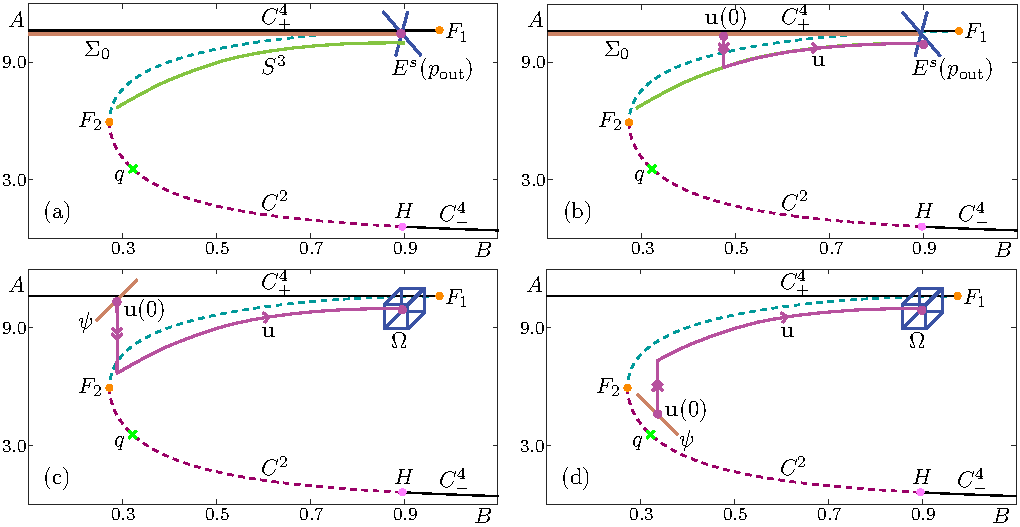
\includegraphics[]{./figures/MKMO_3.pdf}
\caption{A sketch in projection onto the $(B,A)$-plane of the numerical set-up for the computation of submanifolds of $W^s(S^3)$.  Also shown are $C^2$, $C^3$, $C^4_\pm$, $F_1$, $F_2$, $H$ and $q$.  Panel~(a) shows a sketch at the start of the first homotopy step for computing $W^{s}_{\Sigma_0}$ with $S^3$ (green curve), $E^s(p_{\text{out}})$ (blue cross), and the plane $\Sigma_0$ (mocha line) defined by the $A$- and $Y$-coordinates of the point $p_{\text{out}}$.  Panel~(b) shows a representative orbit segment $\mathbf{u}$ (magenta curve) of the first homotopy step.  Panel~(c) shows an illustration of the selection of $\mathbf{u}$ with maximal integration time that starts at $\psi$ (mocha line) and ends on $\Omega$ (blue cube); here the one-dimensional subset $\psi \subset \Sigma_0$ is defined by fixing $B = B_{\text{in}}$ and $\Omega$ is spanned by $E^s(p_{\text{out}})$ and a vector in the $B$-direction. Panel~(d) is a sketch of the selection of a different submanifold $W^{s}_{\Sigma}$ for $\Sigma$ on the other side of the critical manifold.}
\label{figure_3}
\end{figure}
%%%%%%%%%%%%%%%%%%%%%%%%%%%%%%%%%%%%%%%%%%%%%%%%%%%%%%%%%%

Figure~\ref{figure_3} illustrates, step-by-step in projection onto the $(B,A)$-plane, the homotopy steps for computing $W^s_\Sigma$.  Each panel shows the branches $C^2$, $C^3$, and $C^4_\pm$ from Figure~\ref{figure_1} with additional information for the computation. Panels~(a)--(c) of  Figure~\ref{figure_3} illustrate the set-up for obtaining a first solution on $W^s_{\Sigma_0}$ via homotopy steps.  The point $p_{\text{out}}=\begin{pmatrix} 10.6, 0.9, 0.0492, 0.000230 \end{pmatrix}$ with $p_B=0.9$ lies approximately on $C^3$ and the section $\Sigma_0=\{\omega \in \mathbb{R} \; | \;  \omega_A=10.6, \omega_Y=0.000230\}$ intersects $E^s(p_\text{out})$ at the point $p_{\text{out}}$.  We impose condition \eqref{general_conditions_1}, that is, we impose two restrictions on the start point $\mathbf{u}(0)$ of the orbit segment $\mathbf{u}$ because $\Sigma_0$ is two dimensional.  To find a unique $\mathbf{u}$ satisfying \eqref{general_conditions_2} we impose condition \eqref{specific_BC} so that $\mathbf{u}(1)$ is determined by two restrictions.  Hence, the overall 2PBVP is well defined.  Note that $E^s(p_{\text{out}})$ is transverse to $W^u(S^3)$.  In Figure~\ref{figure_3}(a) $\Sigma_0$ is sketched as a mocha curve directly under $C^4_+$, intersecting $E^s(p_{\text{out}})$ which is sketched as a blue cross (note that in panels~(a)--(b), $\Sigma_0$ is shown slightly lower for visibility).  By construction, the point $p_{\text{out}}$ is a solution of the 2PBVP defined by \eqref{equation_4}, \eqref{general_conditions_1}, and \eqref{specific_BC} with $T=0$.

We then increase the total integration time while allowing the $B$-value of $\mathbf{u}(0)$ to decrease towards $F_2$.  Figure~\ref{figure_3}(b) shows an intermediate orbit segment with a fast segment followed by a slow segment along $S^3$.  Panel~(c) shows $\mathbf{u}$ when the continuation is halted at $\mathbf{u}(0)_B = B_{\text{in}}=0.275$, just before $\mathbf{u}(0)_B$ reaches the $B$-coordinate value of $F_2$.  The three-dimensional space $\Omega$ from condition \eqref{general_conditions_2} is shown as a blue cube and $\psi$ from \eqref{BCSTOP} is shown as a mocha line.
    
The orbit segment illustrated in Figure~\ref{figure_3}(c) belongs to a two-parameter family of solutions $\mathbf{u}$ of \eqref{equation_4} that satisfy the boundary conditions \eqref{general_conditions_1} and \eqref{general_conditions_2} for $\Sigma=\Sigma_0$.  In the case where we would like to compute $W^{s}_{\Sigma}$ for $\Sigma$ defined by different $A$ and $Y$ (or $X$) we perform an additional homotopy step to move $\Sigma$.  This can be achieved, after the first homotopy step, by imposing \eqref{general_conditions_1} and \eqref{specific_BC} on an intermediate orbit segment while keeping $T$ and $\mathbf{u}(0)_X$ (or $\mathbf{u}(0)_Y$) as free parameters.  We continue $\mathbf{u}$ while increasing or decreasing the $A$- and/or $Y$-values (or $X$-values) defining $\Sigma$ until we reach the desired plane.  We then also decrease $\mathbf{u}(0)_B$ and stop the continuation when $\mathbf{u}(0)_B = B_{\text{in}}$.  Depending on $\Sigma$, the value of $B_{\text{in}}$ may need to be increased to avoid $\Sigma$ intersecting $C$.  Panel~(d) shows an example of a different choice of $\Sigma$ defined by a smaller value of $A$.  The final step in the homotopy approach determines an orbit segment $\mathbf{u}$ that satisfies \eqref{equation_4}, \eqref{general_conditions_1}, \eqref{general_conditions_2}, and \eqref{general_conditions_3} where $T^B$ is the maximal integration time for solutions with $\mathbf{u}(0)_B=B_p$.

Note that \eqref{general_conditions_2} is automatically satisfied for any solution that satisfies \eqref{specific_BC}.  To find the appropriate value for $T^B$, we require \eqref{BCSTOP} which imposes three conditions on $\mathbf{u}(0)$ and is, hence, more restrictive than \eqref{general_conditions_1}.  We now track the solution $\mathbf{u}$ of the 2PBVP \eqref{equation_4}, \eqref{general_conditions_2}, and \eqref{BCSTOP} as $T$ increases, forcing $\mathbf{u}(0)$ to approach $W^s(S^3)\cap\Sigma$ and $\mathbf{u}(1)$ to approach $W^u(S^3) \cap \Omega$. When a fold in $T$ is detected, a (local) maximum $T_B$ of the total integration time $T$ is attained.

The orbit segment that is obtained is the desired $\mathbf{u}$ with maximal integration time.  It is not represented in a figure because it is practically identical to the orbit segment illustrated in Figure~\ref{figure_3}(c): it begins in $\Sigma$ and has a fast approach to $S^3$ before remaining $O(\varepsilon)$ close for $O(1)$ slow time.  By definition it is an orbit segment in $W^{s}_{\Sigma}$.  In addition to finding an orbit segment that approximates a solution to \eqref{equation_4} contained in $W^s_{\Sigma}$, we can approximate $S^3$ by restricting the orbit segment further to lie entirely inside $(B_{\text{in}},B_{\text{out}})$ to exclude fast segments.

%%%%%%%%%%%%%%%%%%%%%%%%%%%%%%%%%%%%%%%%%%%%%%%%%%%%%%%%%%
\begin{figure}[t!]
\centering
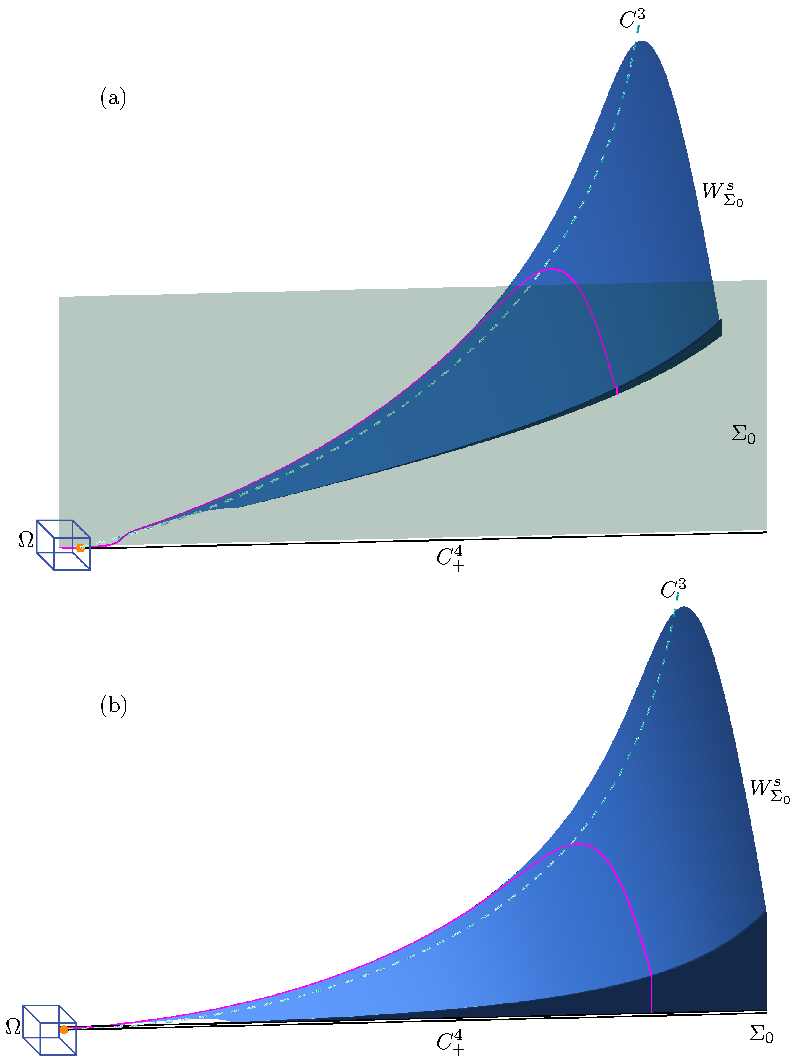
\includegraphics[]{./figures/MKMO_4.pdf}
\caption{The submanifold $W^{s}_{\Sigma_0}$ (light-blue surface) of $W^s(S^3)$, shown in projection onto the $(B,A,X)$-space (a) and onto the $(B,A,Y)$-space (b); also shown are a representative orbit segment $\mathbf{u}$ (magenta curve), the plane $\Sigma_0$ (mint surface and line), $\Omega$ (represented by a blue cube), $C^3$, $C^4_+$, and $F_1$.}
\label{figure_4}
\end{figure}
%%%%%%%%%%%%%%%%%%%%%%%%%%%%%%%%%%%%%%%%%%%%%%%%%%%%%%%%%%

After these homotopy steps we use \eqref{general_conditions_1}, \eqref{general_conditions_2}, and \eqref{general_conditions_3} to sweep out a one-parameter family of solutions which gives an accurate approximation of $W^s_\Sigma$.  Here, $T^B$ is adjusted so that it remains a fold point for $T$ as $B$ varies. Figure~\ref{figure_4} shows $W^s_{\Sigma_0}$ (light-blue surface) in projection onto the $(B,A,X)$-space in panel~(a) and onto the $(B,A,Y)$-space in panel~(b) with $\Sigma_0$ (mint surface and line); the plane $\Sigma_0$ appears as a line in panel~(b) because it is defined by constant $A$ and $Y$.  The view is rotated relative to earlier figures to help illustrate the geometry of this submanifold.  Also shown are $C^3$, $C^4_+$, $F_1$, and $\Omega$.  Although the manifold is two dimensional, it is necessary to visualise it in both $(B,A,X)$- and $(B,A,Y)$-projections because it exists in a four-dimensional space.  Shown on $W^s_{\Sigma_0}$ is an orbit segment $\mathbf{u}$ (magenta curve) representative of those used to compute $W^s_{\Sigma_0}$.  The orbit segment $\mathbf{u}$ starts at a given $B$ and ends at $\Omega$ with maximum integration time.  It has a fast approach to $S^3$ in $X$ and $Y$ before approaching mainly in the $A$-direction and then, finally, remaining close to $C^3$ for $O(1)$ slow time; this is evidence of a time-scale splitting  between $A$, and $X$ and $Y$.

%%%%%%%%%%%%%%%%%%%%%%%%%%%%%%%%%%%%%%%%%%%%%%%%%%%%%%%%%%
\begin{figure}[t!]
\centering
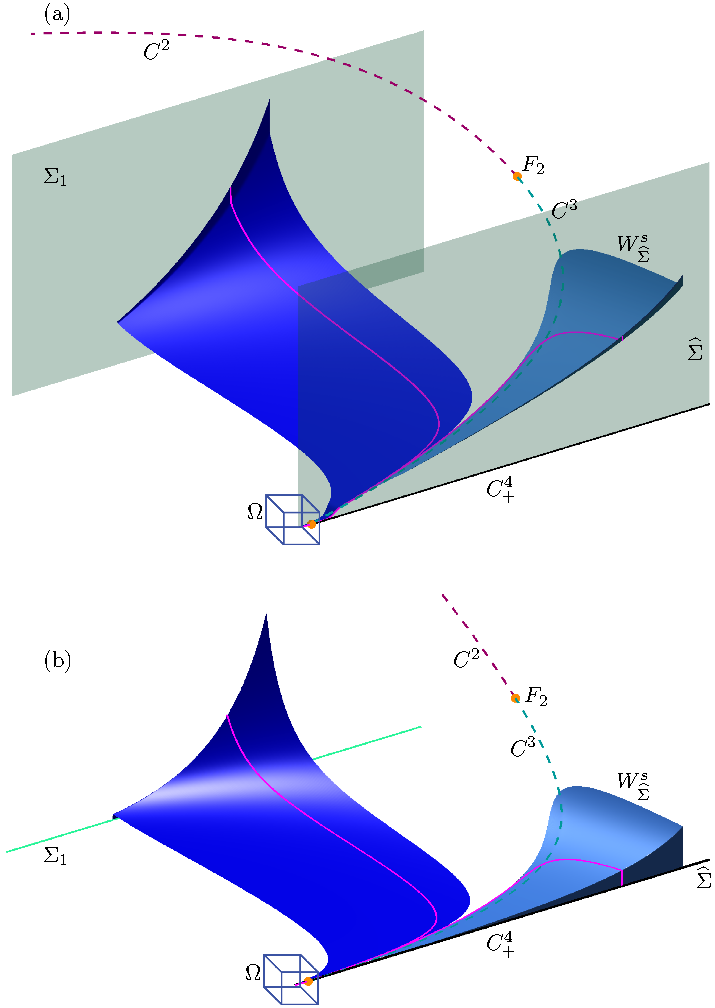
\includegraphics[]{./figures/MKMO_5.pdf}
\caption{The submanifolds $W^{s}_{\Sigma_0}$ (blue surface) and $W^{s}_{\Sigma_0}$ (light-blue surface) of $W^s$, shown in projection onto the $(B,A,X)$-space (a) and onto the $(B,A,Y)$-space (b); also shown are representative orbit segments $\mathbf{u}$ (magenta curves), the planes $\Sigma_0$ (mint surface and line) and $\Sigma_1$ (mint surface and line), and $\Omega$ (represented by a blue cube), $C^2$, $C^3$, $C^4_+$, $F_1$, and $F_2$.}
\label{figure_5}
\end{figure}
%%%%%%%%%%%%%%%%%%%%%%%%%%%%%%%%%%%%%%%%%%%%%%%%%%%%%%%%%%

Figure~\ref{figure_5} shows $W^s_{\Sigma_0}$ (light-blue surface) together with one other submanifold $W^{s}_{\Sigma_1}$ (blue surface) of $W^{s}$ in projection onto the $(B,A,X)$-space in panel~ (a) and onto the $(B,A,Y)$-space in panel~ (b); here $\Sigma_1$ (mint surface) is given by $A=2.0$ and $Y=0.0$.  The surface $\Sigma_1$ appears as a line in panel~(b) because it is defined by constant $A$ and $X$.  The submanifold $W^s_{\Sigma_1}$ is an example of a submanifold on the other side of $C$ with respect to the variable $A$; compare with Figure~\ref{figure_3}(d).  A representative magenta orbit segment on $W^s_{\Sigma_1}$ is shown approaching $S^3$ first mainly from the $X$- and $Y$-directions, before approaching mostly in the $A$-direction.

%%%%%%%%%%%%%%%%%%%%%%%%%%%%%%%%%%%%%%%%%%%%%%%%%%%%%%%%%%
\begin{figure}[t!]
\centering
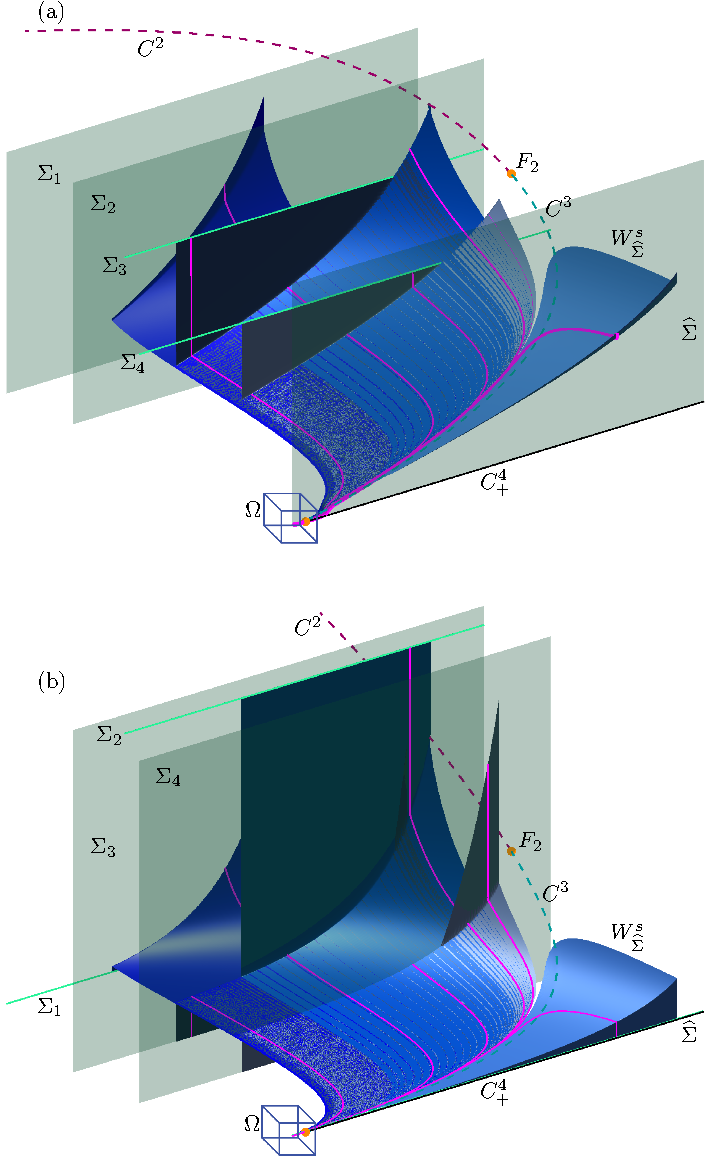
\includegraphics[]{./figures/MKMO_6.pdf}
\caption{The submanifolds from Figure~\ref{figure_5} with three additional submanifolds $W^s_{\Sigma_i}$ (blue surfaces) of $W^s$ for $2 \leq i \leq 4$ in projection onto the $(B,A,X)$-space (a) and the $(B,A,Y)$-space (b); also shown are representative orbit segments $\mathbf{u}$ (magenta curves), the planes $\Sigma_i$ (mint surfaces and lines), and $\Omega$ (represented by a blue cube), $C^2$, $C^3$, $C^4_+$, $F_1$, and $F_2$.}
\label{figure_6}
\end{figure}
%%%%%%%%%%%%%%%%%%%%%%%%%%%%%%%%%%%%%%%%%%%%%%%%%%%%%%%%%%

Figure~\ref{figure_6} shows the two submanifolds of $W^{s}$ from Figure~\ref{figure_5} with three additional submanifolds $W^s_{\Sigma_i}$ (blue surfaces), $2 \leq i \leq 4$, and the corresponding planes $\Sigma_i$ (mint surfaces) that define them.  Also shown are $C^3$, $C^4_+$, $F_1$, and $\Omega$.  The additional submanifolds were selected as follows: $\Sigma_2$ is given by $A=4.0$ and $Y=0.75$, $\Sigma_3$ is given by $A=4.0$ and $X=0.75$, and $\Sigma_4$ is given by $A=6.0$ and $X=0.5$.  Note that  $\Sigma_3$ and $\Sigma_4$ appear as lines in panel~(a) because they are defined by constant $A$ and $X$.  Similarly, $\Sigma_2$ appears as a line in panel~(b) because it is defined by constant values of $A$ and $Y$.  Orbit segments in Figure~\ref{figure_6} again first approach $S^3$ in the $X$- and $Y$-directions before approaching in the $A$-direction.  Consequently, there are regions where different submanifolds are extremely close to each other.  In fact, these surfaces are so close that \textsc{Matlab} (which we use for our visualization throughout) cannot distinguish them properly.  Different choices of $B_{\text{in}}$ and $B_{\text{out}}$ also cause some submanifolds to extend farther than others in the $B$-direction.

Overall this section and its figures demonstrate that we can reliably compute any number of submanifolds $W^s_\Sigma$ with conditions \eqref{general_conditions_1},  \eqref{general_conditions_2} and \eqref{general_conditions_3}, and the homotopy steps outlined above.  Together, these two-dimensional submanifolds provide an understanding of the dynamics inside $W^s(S^3)$.


%%%%%%%%%%%%%%%%%%%%%%%%%%%%%%%%%%%%%%%%%%%%%%%%%%%%%%%%%%
\subsection{Definition and computation of $W^{u}(S^2)$}  
\label{sec:compWuS2}

We can define $S^2$ and $W^u(S^2)$ similarly to how we defined $S^3$ and $W^s(S^3)$.  The values for $B_{\text{in}}$ and $B_{\text{out}}$ are chosen such that $[B_{\text{out}}, B_{\text{in}}] \subset (B_q, B_H)$, where $B_q \approx 0.323$ and $B_H \approx 0.897$ are the $B$-values of the saddle equilibrium $q$ and the Hopf point $H$ shown as a green cross and a pink dot, respectively, in Figures~\ref{figure_1}, \ref{figure_3}, and~\ref{figure_7}. Note that in these figures, the flow near $S^2$ is toward $q$; hence, to the right of $W^u(q)$ the flow is to the left.  Our choice of $B_{\text{out}}>B_{q}$ is to avoid a change in direction of the flow associated with $q$.

To compute a submanifold of $W^{u}(S^2)$ we use slightly different boundary conditions and homotopy steps compared to those used for $W^s(S^3)$ in light of two complicating challenges arising from $q$ and $H$.  Orbit segments near $S^2$ may increase in integration time by approaching $W^s(q)$ or by following the attracting slow manifold associated with $C^4_-$ backwards in time.  We define a submanifold of $W^u(S^2)$ with boundary conditions that ensure that computed orbit segments do not demonstrate these behaviors and only increase in integration time by approaching $S^2$.  

To define $S^2$ and $W^u(S^2)$, we define a three-dimensional cylinder $\mathscr{D}^u$ that is transverse to the flow and to $E^s(C^2)$.  To this end, we choose a radius $r$ and for each $B_p \in [B_{\mathrm{in}}, B_{\mathrm{out}}]$ define the two-dimensional sphere in the subspace $\{\omega \in \mathbb{R}^4 \; | \; B=B_p\}$ centred at $p$ and with radius $r$; here $p \in C^2$ is the unique point such that $p_B = B_p$.  More formally,
%
\begin{equation*}
D^u_r(B_p)=\{w \in \mathbb{R}^4 \;|\; w_B = B_p, \left\lVert w-p \right\lVert  = r\}.
\end{equation*}
%
Then 
%
\begin{equation*}
\mathscr{D}^u = \bigcup\limits_{B_p \in [B_{\mathrm{out}}, B_{\mathrm{in}}]}^{}D^u_r(B),
\end{equation*}
%
is a three-dimensional cylinder.  We now consider the smooth, one-parameter family of orbit segments of \eqref{equation_1} given by the property that each orbit segment remains inside $\mathscr{D}^u$ for an O(1) amount of slow time, exits $\mathscr{D}^u$ via $D^u_r(B_p)$ for some $B_p \in [B_{\text{out}}, B_{\text{in}}]$ and ends in some plane $\Sigma$.  We denote by $W^u_\Sigma$ those parts of the orbit segments that exit $\mathscr{D}^u$ in the fast direction.  The earlier parts that evolve mostly in the $B$-direction inside $\mathscr{D}^u$ for $O(1)$ slow time are approximate segments of $S^2$.  If such an earlier part of the orbit segment includes a fast entrance into $\mathscr{D}^u$, that fast part lies on $W^s(S^2)$ in good approximation.

We compute the submanifold $W^u_\Sigma$ again as a one-parameter family of orbit segments $\mathbf{w}$ satisfying the rescaled equation \eqref{equation_4}.  Orbit segments $\mathbf{w} \in W^u_\Sigma$ must satisfy the boundary conditions
%
\begin{equation}
	\mathbf{w}(1) \in \Sigma,
	\label{general_conditions_unstable_1}
\end{equation}
%
\begin{equation}
	\mathbf{w}(0) \in \Phi = E^u(p_0) \times \begin{bmatrix} 0, 1, 0, 0 \end{bmatrix}^{\rm tr},
\label{general_conditions_unstable_2}
\end{equation}
%
\begin{equation}
	\mathbf{w}(0)_B = \widehat{B},
	\label{general_conditions_unstable_3}
\end{equation}
%
where $p_0 \in C^2$ is such that $p_{0_B} \in (B_{\text{out}}, B_{\text{in}})$ and $\widehat{B}>B_{\text{in}}$.  Equations \eqref{general_conditions_unstable_1} and \eqref{general_conditions_unstable_2} are analogous to equations \eqref{general_conditions_1} and \eqref{general_conditions_2} from Section~\ref{sec:compWsS3}.  Equation \eqref{general_conditions_unstable_3} serves the purpose of preventing $\mathbf{w}$ from increasing in integration time by following the attracting slow manifold associated with $C^4_-$ backward in time; it has no analogue in Section~\ref{sec:compWsS3}. Equations \eqref{general_conditions_unstable_1}, \eqref{general_conditions_unstable_2}, and \eqref{general_conditions_unstable_3} define four conditions on solutions of \eqref{equation_4} so that there is a well-defined one-parameter family of solutions to this 2PBVP, which represents $W^u_\Sigma$.

Note that the above conditions preclude the selection of $\mathbf{w}$ with maximal integration time as was done in Section~\ref{sec:compWsS3} with equation \eqref{general_conditions_3}.  In the case that we would like to impose a condition of maximum integration time, we may substitute for \eqref{general_conditions_unstable_1} the two conditions
%
\begin{equation}
	\mathbf{w}(1) \in \mathscr{D}^u,
	\label{general_conditions_unstable_4}
\end{equation}
%
and
%
\begin{equation}
	T = T^B,
	\label{general_conditions_unstable_5}
\end{equation}
%
where for each $B_p \in [B_{\text{out}}, B_{\text{in}}]$, the time $T^B$ is determined as a fold point corresponding to the maximum integration time of an orbit segment that exits $\mathscr{D}^u$ at $B = B_p$ while satisfying \eqref{general_conditions_unstable_2} and \eqref{general_conditions_unstable_3}.  Indeed, equation \eqref{general_conditions_unstable_4} imposes one condition on $\mathbf{w}(1)$, one condition less than equation \eqref{general_conditions_unstable_1}, allowing us also to impose equation \eqref{general_conditions_unstable_5}.  Equations \eqref{general_conditions_unstable_2}, \eqref{general_conditions_unstable_3}, \eqref{general_conditions_unstable_4}, and \eqref{general_conditions_unstable_5} define four conditions on solutions of \eqref{equation_4} so that there is again a one-parameter family of solutions to this 2PBVP.  We denote the two-dimensional submanifold given by this one-parameter family by $W^u_r$.

Once an initial $\mathbf{w}$ satisfying one of the 2PBVPs  is found, it is possible to sweep out a submanifold $W^u_\Sigma$ or $W^u_r$ by continuing $\mathbf{w}$ with varying $\mathbf{w}(1)_B$ and $T_B$.  The challenge is, once again, the computation via homotopy steps of an initial orbit segment satisfying the boundary conditions.

In the first homotopy step, we choose the point $p_0=\begin{pmatrix} p_{0_A}, p_{0_B}, p_{0_X}, p_{0_Y} \end{pmatrix} \in C^2$ by fixing $p_{0_B}=B_0 \in [B_{\text{out}}, B_{\text{in}}]$.  We impose condition \eqref{general_conditions_unstable_2} as well as the condition
%
\begin{equation}
		\mathbf{w}(1) \in \chi = \{ \omega \in \mathbb{R}^4 \; | \; \omega_A=p_{0_A}, \omega_B=p_{0_B}, \omega_Y=p_{0_Y} \}.
		\label{specific_BC_unstable1}
\end{equation}
%
The point $p_0$ is then a solution to \eqref{general_conditions_unstable_2} and \eqref{specific_BC_unstable1} for $T=0$.  We increase $\mathbf{w}_B$ with $T$ as a free parameter and stop the continuation when $\mathbf{w}_B=\widehat{B}$.  The value of $\mathbf{w}_B$ is fixed from this step onwards.  We define the two-dimensional space
%
\begin{equation*}
	\Phi_{\widehat{B}} = \Phi \cap \{ \omega \in \mathbb{R} \; | \; \omega_B=\widehat{B}\}.
\end{equation*}

In the second homotopy step, we substitute equation \eqref{specific_BC_unstable1} for \eqref{general_conditions_unstable_1} with $\Sigma=\{ \omega \in \mathbb{R}^4 \;|\; \omega_A=p_{0_A}, \omega_Y=p_{0_Y} \}$ and impose \eqref{general_conditions_unstable_3}.  The orbit segment $\mathbf{w}$ at the end of the first homotopy step is then a solution to this 2PBVP defined by \eqref{equation_4}, \eqref{general_conditions_unstable_1}, \eqref{general_conditions_unstable_2}, and \eqref{general_conditions_unstable_3}.  It is in this second homotopy step that we decide whether to compute a submanifold $W^u_\Sigma$ or $W^u_r$.  If our aim is to compute $W^u_\Sigma$, all that remains to compute an initial $\mathbf{w}$ lying on the manifold is to move $\Sigma$ to a desired location, as in Section~\ref{sec:compWsS3}.  To compute $W^u_r$ we increase $T$ until $\mathbf{w}(1) \in \Sigma \cap \mathscr{D}^u$.  This is detected as $\mathbf{w}(1)$ reaching a distance of $r$ away from the point $p \in C^2$ such that $p_B = \mathbf{w}_B$.  We denote the coordinates $\mathbf{w}(1)_B$ and $\mathbf{w}(1)_X$ of the end point at the end of this step by $\widetilde{B}$ and $\widetilde{X}$, respectively.  

In the event that $D_r(\widetilde{B})$ contains a locus of points at which the flow is tangent to it, we perform a third homotopy step to increase $\widetilde{B}$ until the flow is transverse to $D_r(\widetilde{B})$.  This is achieved by imposing conditions \eqref{general_conditions_unstable_2}, \eqref{general_conditions_unstable_3}, and \eqref{general_conditions_unstable_4} on $\mathbf{w}$ at the end of the second homotopy step and then increasing $\mathbf{w}_B$ while keeping $T$ as a free parameter.

In the final homotopy step, we replace condition \eqref{general_conditions_unstable_4} with 
%
\begin{equation}
		\mathbf{w}(1) \in \Theta = D^u_r(\widetilde{B}) \cap \{ \omega \in \mathbb{R} \; | \; \omega_X = \widetilde{X} \}.
		\label{specific_BC_unstable2}
\end{equation}
%
The orbit segment $\mathbf{w}$ at the end of the second homotopy step (or the third homotopy step if one was necessary) is then a solution to the 2PBVP defined by \eqref{equation_4}, \eqref{general_conditions_unstable_2}, \eqref{general_conditions_unstable_3}, and \eqref{specific_BC_unstable2}.    We now increase $T$ until $T=T^B$, which is detected as a fold in integration time.  The resulting orbit segment $\mathbf{w}$ lies on $W^u_r$.

Once an initial orbit segment $\mathbf{w}$ on either $W^u_\Sigma$ or $W^u_r$ is found, we may sweep out the remaining part of the submanifold by increasing and decreasing $\mathbf{w}_B$ and keeping $T^B$ as a free parameter so that it is adjusted accordingly to satisfy the fold condition.

%%%%%%%%%%%%%%%%%%%%%%%%%%%%%%%%%%%%%%%%%%%%%%%%%%%%%%%%%%
\begin{figure}[t!]
\centering
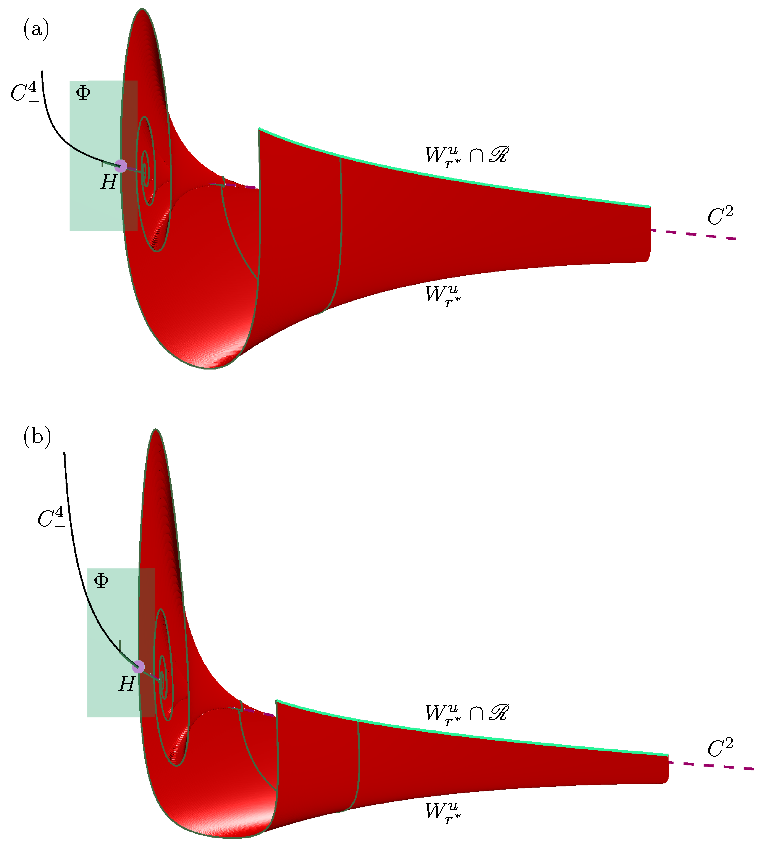
\includegraphics[]{./figures/MKMO_7.pdf}
\caption{A sketch in projection onto the $(B,A)$-plane of the homotopy steps for the computation of submanifolds $W^u_r$ of $W^u(S^2)$.  Also shown are $C^2$ (dashed raspberry curve), $C^4_-$ (black curve), $H$ (pink dot), $q$ (green cross), and the orbit segment $\mathbf{w}$ (forest green curve).  Panel~(a) is a sketch of the situation during the first homotopy step with $\chi$ (mint line) and $\Phi$ (mint prism); panel~(b) is a sketch of the start of the final homotopy step with $\Theta$ (mint circle) and $\Phi_{\widehat{B}}$ (mint cross).}
\label{figure_7}
\end{figure} 
%%%%%%%%%%%%%%%%%%%%%%%%%%%%%%%%%%%%%%%%%%%%%%%%%%%%%%%%%%

Figure~\ref{figure_7} illustrates, in projection onto the $(B,A)$-plane, the adjusted homotopy steps for computing $W^u_r$.  Each panel shows an enlargement of the critical manifold $C$ from Figure~\ref{figure_1} near $C^2$ with additional information for the computation.   We choose $p_0=\begin{pmatrix} 0.940272, && 0.7, && 1.492271, && 1.342954 \end{pmatrix}$ which lies approximately on $C^2$.  In the first homotopy step, we impose condition \eqref{specific_BC_unstable1}, which imposes three conditions on $\mathbf{w}(1)$, as well as condition \eqref{general_conditions_unstable_2}, which imposes one restriction on $\mathbf{w}(0)$.  Panel~(a) shows a sketch of an intermediate situation in the first homotopy step; here, we show $\mathbf{w}$ (forest green curve), the one-dimensional line $\chi$ sketched in mint, and the three-dimensional $\Phi$ sketched as a mint prism.  The $B$-coordinate of $\mathbf{w}(0)$ is increased with $T$ as a free parameter.  The continuation is stopped when $\mathbf{w}(0)_B=\widehat{B}$ for $\widehat{B}=1.0$.  In the second homotopy step, we impose \eqref{general_conditions_unstable_1}, \eqref{general_conditions_unstable_2}, and \eqref{general_conditions_unstable_3}, increasing $\mathbf{w}(1)_B$ with $T$ as a free parameter until $\mathbf{w}(1)$ intersects $\mathscr{D}^u$ for $r=0.7$.  We are not required to perform an additional homotopy step because $D_r(\widetilde{B})$, in this case, does not contain a locus of points at which the flow is tangent to it.  Figure~\ref{figure_7}(b) shows a sketch of the numerical set up before the final homotopy step; here, the one-dimensional closed curve $\Theta$ is sketched in mint and $\Phi_{\widehat{B}}$ is sketched as a mint cross. We then impose \eqref{general_conditions_unstable_2}, \eqref{general_conditions_unstable_3}, \eqref{general_conditions_unstable_4} and \eqref{general_conditions_unstable_5} and increase $T$.  The continuation is stopped when $T=T^B$ which is again detected as a fold.  The resulting orbit segment lies on $W^u_r$.  We can then sweep out the rest of the submanifold $W^u_r$ by continuing the fold in integration time for increasing and decreasing $\mathbf{w}(1)_B$.

%%%%%%%%%%%%%%%%%%%%%%%%%%%%%%%%%%%%%%%%%%%%%%%%%%%%%%%%%%
\begin{figure}[t!]
\centering
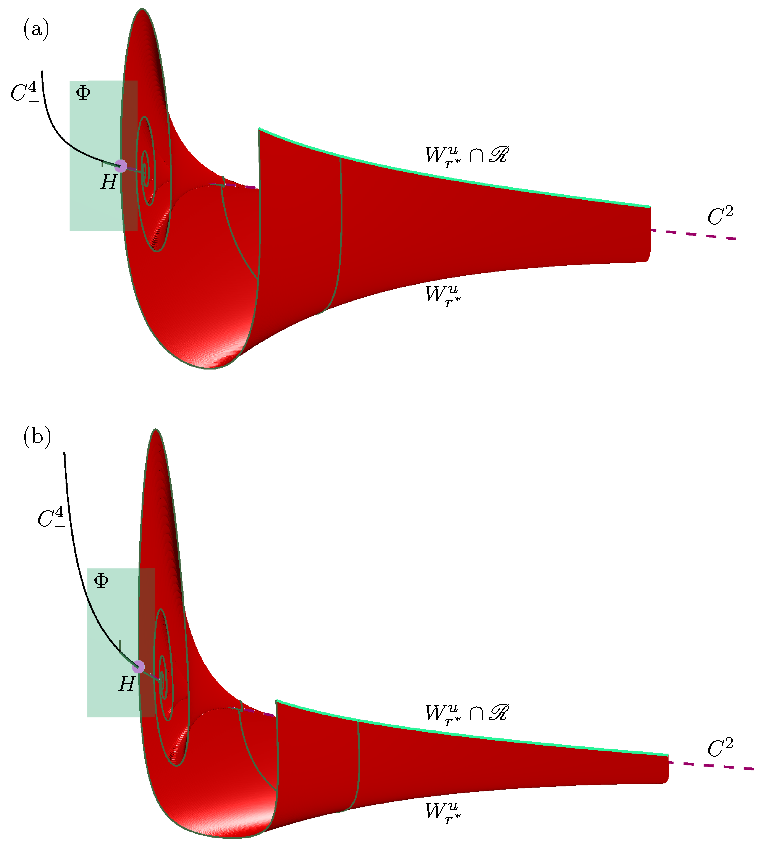
\includegraphics[]{./figures/MKMO_8.pdf}
\caption{The submanifold $W^u_{r}$ (red surface) of $W^u(S^2)$ for $r=0.7$ shown in projection onto $(B,A,X)$-space (a) and $(B,A,Y)$-space (b); note that the view is rotated compared to previous figures.  Also shown are two representative orbit segments $\mathbf{w}$ (forest green curves) on $W^u_{r}$, the two-dimensional space $\Phi_{\widehat{B}}$ (mint surface), the one-dimensional intersection $W^s_{r}\cap\mathscr{D}^u$ (mint curve), along with the curves $C^2$ and $C^4_-$, and the point $H$.}
\label{figure_8}
\end{figure}
%%%%%%%%%%%%%%%%%%%%%%%%%%%%%%%%%%%%%%%%%%%%%%%%%%%%%%%%%%

Figure~\ref{figure_8} shows two projections of the submanifold $W^u_{r}$ for $r=0.7$ with $W^u_{r} \cap \mathscr{D}^u$ (mint curve) and $\Phi_{\widehat{B}}$ (mint surface).  Note that $W^u_{r}\cap\mathscr{D}^u$ is simply the curve traced out by $\mathbf{w}(1)$.  To facilitate viewing, the view is rotated compared to previous figures.  Two representative orbit segments $\mathbf{w}$ are plotted and a subset of $C^2$ (dashed raspberry curve) is shown.  From this angle, the radius of $\mathscr{D}^u$ may, to some readers, appear to decrease with decreasing $\mathbf{w}(1)_B$.  This is due to the eye's erroneous association of points $\mathbf{w}(1)$ with points $p \in C^2$ such that $p_B < \mathbf{w}(1)_B$.  Due to the spiralling nature of $W^u_r$, we only show one such submanifold in our visualization.


%%%%%%%%%%%%%%%%%%%%%%%%%%%%%%%%%%%%%%%%%%%%%%%%%%%%%%%%%%
\section{A heteroclinic connection between two saddle slow manifolds}
\label{sec:hetconn}

Two three-dimensional objects in a four-dimensional space may intersect generically in a two-dimensional manifold.  It follows, then, that the three-dimensional $W^s(S^3)$ and the three-dimensional $W^u(S^2)$ may intersect in a two-dimensional surface of heteroclinic connections.  This is supported by the fact that, for the reduced system in \cite{QSSA}, there exists a two-dimensional stable manifold associated with the branch equivalent to $C^3$ that stretches backward in time all the way to the branch equivalent to $C^2$.  Hence, we wish to detect and compute a surface of connections, which we denote $\mathscr{H}$.  A natural way forward is to consider $\mathscr{H}$ as a one-parameter family of concatenations of orbit segments $\mathbf{w} \in W^u(S^2)$ with $\mathbf{u} \in W^u(S^3)$.

%%%%%%%%%%%%%%%%%%%%%%%%%%%%%%%%%%%%%%%%%%%%%%%%%%%%%%%%%%
\begin{figure}[t!]
\centering
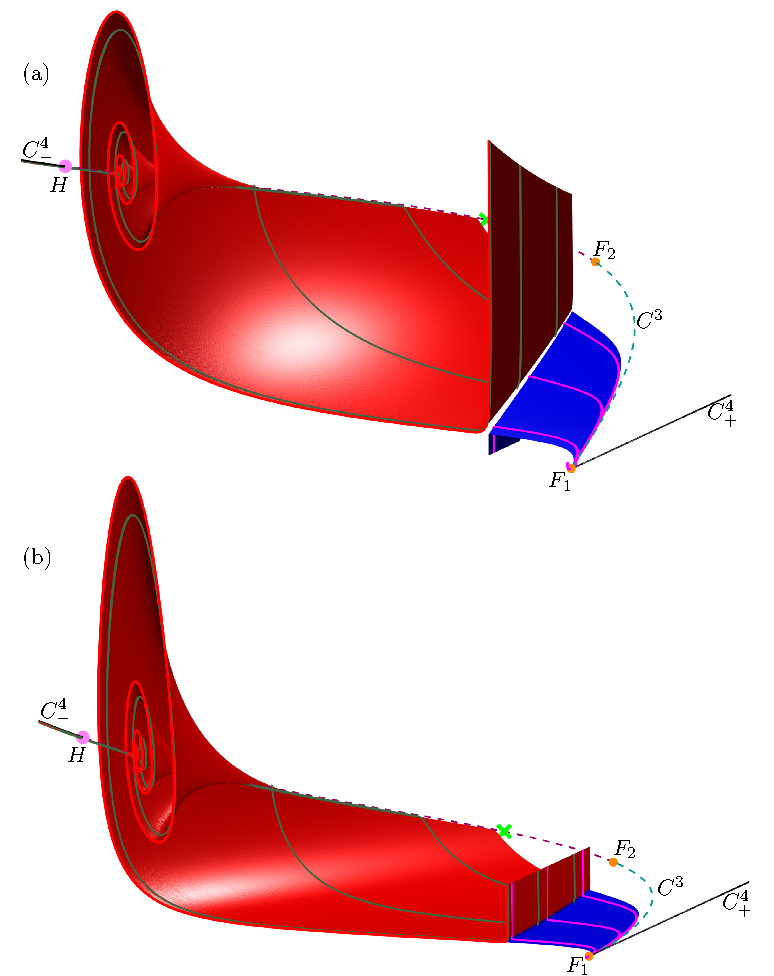
\includegraphics[]{./figures/MKMO_9.pdf}
\caption{The submanifold $W^u_{\Sigma_5}$ (red surface) of $W^u(S^2)$ and the submanifold $W^s_{\Sigma_5}$ (blue surface) of $W^s(S^3)$ in projection onto $(B,A,X)$-space (a) and onto $(B,A,Y)$-space (b). Representative orbit segments $\mathbf{w} \in W^u_{\Sigma_5}$ and $\mathbf{u} \in W^u_{\Sigma_5}$ are plotted in forest green and magenta, respectively; also shown are $C^2$, $C^3$, $C^4_\pm$, $F_1$, $F_2$, $H$, and $q$ (which is partially obscured by the two-dimensional submanifold $W^u_{\Sigma_5}$). }
\label{figure_9}
\end{figure}
%%%%%%%%%%%%%%%%%%%%%%%%%%%%%%%%%%%%%%%%%%%%%%%%%%%%%%%%%%

A first idea is to compute two two-dimensional submanifolds $W^u_\Sigma$ and $W^s_\Sigma$ up to a suitable choice of a single two-dimensional section $\Sigma$.  However, these two two-dimensional objects do not generically intersect in a four-dimensional space.  Figure~\ref{figure_9} demonstrates this difficulty.  The chosen section $\Sigma_5=\{\omega \in \mathbb{R}^4 \;|\; \omega_A= 6.0, \omega_Y=0.5 \}$ yields the submanifolds $W^s_{\Sigma_5}$ (blue surface) and $W^u_{\Sigma_5}$ (red surface) shown in Figure~\ref{figure_9}.  Representative orbit segments $\mathbf{w}$ (forest green curves) and $\mathbf{u}$ (magenta curves) are shown coming toward each other mostly in the $A$-direction before diverging away from each other in the faster $X$- and $Y$-directions.  Although the submanifolds appear to intersect in the $(B,A,Y)$-projection in Figure~\ref{figure_9}(b), we can see from the $(B,A,X)$-projection in Figure~\ref{figure_9}(a) that the surfaces $W^s_{\Sigma_5}$ and $W^u_{\Sigma_5}$, in fact, miss each other in the four-dimensional phase space.  Nevertheless, we are encouraged by the closeness of $W^u_{\Sigma_5}$ and $W^s_{\Sigma_5}$, which suggests that a nearby surface $\mathscr{H}$ of connecting orbits could exist.

We turn to Lin's method to find the actual surface of connecting orbits $\mathscr{H}$.  Lin's method has been used in parameter continuation to locate global connecting orbits between equilibria and/or periodic orbits \cite{Lin_original, Lin_POs, Lin_POs2}.  We use it here in a novel way to locate structurally stable connections between $S^2$ and $S^3$ for the system parameters given in the four-dimensional space of system \eqref{equation_1}.

We begin by choosing a three-dimensional section $\mathscr{L}$, called a Lin section, that divides the four-dimensional phase space into two regions such that $C^3$ lies in one region and $C^2$ lies in the other.  More specifically, the Lin section $\mathscr{L}$ is defined by a constant value of $A$ that is chosen so that $\mathscr{L}$ intersects $C$ to the left of $W^u(q)$ in the $(B,A)$-projection; this choice of $\mathscr{L}$ allows us to compute the largest possible portion of $\mathscr{H}$ to the right of $W^u(q)$.  Inside $\mathscr{L}$ we choose a unit vector $\mathbf{v}_Z$ with the generic property that it is not tangent to either $W^u(S^2)$ or $W^s(S^3)$.  The vector $\mathbf{v}_Z$ is called a Lin vector and the space $Z$ spanned by $\mathbf{v}_Z$ the associated Lin space.  We then use the methods outlined in Section~\ref{sec:slowmans} to compute $\mathbf{u} \in W^s(S^3)$ and $\mathbf{w} \in W^u(S^2)$ such that
%
\begin{equation}
	\mathbf{u}(0) \in \mathscr{L}
	\label{general_conditions_heteroclinic_1}
\end{equation}
%
and
%
\begin{equation}	
	 \mathbf{w}(1) \in \mathscr{L}.
	 \label{general_conditions_heteroclinic_2}
\end{equation}
%
Additionally, we require that
%
\begin{equation*}
	\mathbf{u}(0)-\mathbf{w}(1) \in Z.
\end{equation*}
%
Note that the difference $\mathbf{u}(0)-\mathbf{w}(1)$ of arbitrary orbit segments $\mathbf{u} \in W^s(S^3)$ and $\mathbf{w} \in W^u(S^2)$ will typically correspond to a vector direction $\mathbf{v}_Z$ that is transverse to both manifolds.  Hence, we first compute two orbit segments $\mathbf{u}$ and $\mathbf{w}$ on the respective manifolds and then decide on the choice for $\mathbf{v}_Z$.  Importantly, the signed distance between $\mathbf{u}(0)$ and $\mathbf{w}(1)$ inside $Z$, given by
%
\begin{equation}
	\eta=[\mathbf{u}(0)-\mathbf{w}(1)] \cdot \mathbf{v}_Z,
	\label{general_conditions_heteroclinic_3}
\end{equation}
%
is a regular test function.  This means that $\eta$ is a smooth function with (generically) regular zeros, as a function of a single input parameter that determines the choice of the coupled orbit segments $\mathbf{u}$ and $\mathbf{w}$. Note that $\left\lvert \eta \right\lvert = \left\lVert \mathbf{u}(0)-\mathbf{w}(1) \right\lVert$. A pair of orbit segments $(\mathbf{w},\mathbf{u})$ with 
%
\begin{equation}
	\eta = 0
	\label{general_conditions_heteroclinic_4}
\end{equation}
%
is therefore a smooth connecting orbit segment between $S^2$ and $S^3$.  Hence, finding a zero of $\eta$ is the way of finding a (first) connecting orbit in $\mathscr{H}$.

To implement $\mathbf{u}(0), \mathbf{w}(1) \in Z$, we define unit normal vectors $\mathbf{n}_1 \perp \mathbf{v}_Z$ and $\mathbf{n}_2 \perp \mathbf{v}_Z$ in $\mathscr{L}$ such that $\mathbf{n}_1 \perp \mathbf{n}_2$ and impose conditions
%
\begin{equation}
	[\mathbf{u}(0) - \mathbf{w}(1)] \cdot \mathbf{n}_1 =0
	\label{general_conditions_heteroclinic_5}
\end{equation}
%
and
%
\begin{equation}	
	 [\mathbf{u}(0) - \mathbf{w}(1)] \cdot \mathbf{n}_2 =0.
	 \label{general_conditions_heteroclinic_6}
\end{equation}
%
Equations \eqref{general_conditions_heteroclinic_5} and \eqref{general_conditions_heteroclinic_6} ensure that $\mathbf{w}(1)-\mathbf{u}(0)$ remains in $Z$.  Conditions \eqref{general_conditions_heteroclinic_3} and \eqref{general_conditions_heteroclinic_4} together ensure that $\mathbf{w}(1) = \mathbf{u}(0)$.  Once an initial pair of orbit segments $(\mathbf{w}, \mathbf{u})$ satisfying the above conditions is found, the surface $\mathscr{H}$ can be swept out, for example, by varying $\mathbf{w}(1)_B$ as the input parameter with $\mathbf{u}(0)_B$ and $T$ as additional free parameters.  

The challenge is, as always, to find an initial pair $(\mathbf{w}, \mathbf{u})$ satisfying the required boundary conditions via a series of homotopy steps.  In the first homotopy step we compute $\mathbf{w} \in W^u_{\Sigma_{L_1}}$ and $\mathbf{u} \in W^s_{\Sigma_{L_2}}$ for $\Sigma_{L_1} $, $\Sigma_{L_2} \subset \mathscr{L}$, requiring \eqref{general_conditions_1} and \eqref{specific_BC} for $\mathbf{u}$ and \eqref{general_conditions_unstable_1}, \eqref{general_conditions_unstable_2}, and \eqref{general_conditions_unstable_3} for $\mathbf{w}$.  In particular, \eqref{general_conditions_heteroclinic_1} and \eqref{general_conditions_heteroclinic_2} are then satisfied and we choose
%
\begin{equation*}
		\mathbf{v}_Z = \frac{\mathbf{u}(0) - \mathbf{w}(1)}{\left\lVert \mathbf{u}(0) - \mathbf{w}(1) \right\lVert},
		\label{Lin_vector}
\end{equation*}
%
which is a convenient choice of a vector that is (generically) transverse to $W^u(S^2)$ and $W^s(S^3)$. We then find the vectors $\mathbf{n}_1$ and $\mathbf{n}_2$ required for conditions \eqref{general_conditions_heteroclinic_1} and  \eqref{general_conditions_heteroclinic_2}. Once chosen, the vector $\mathbf{v}_Z$ and normal vectors $\mathbf{n}_1$ and $\mathbf{n}_2$ remains fixed throughout the computations.

The conditions imposed in the first homotopy step define a two-parameter family of paired orbit segments $(\mathbf{w}, \mathbf{u})$ that meet in $\mathscr{L}$ along $Z$.  In the second homotopy step, we now relax conditions \eqref{general_conditions_1} and \eqref{general_conditions_unstable_1}, which respectively are two conditions each on $\mathbf{u}$ and $\mathbf{w}$, and impose instead conditions \eqref{general_conditions_heteroclinic_1} and \eqref{general_conditions_heteroclinic_2}, \eqref{general_conditions_heteroclinic_3}, \eqref{general_conditions_heteroclinic_5} and \eqref{general_conditions_heteroclinic_6}.    Conditions \eqref{general_conditions_heteroclinic_1} and  \eqref{general_conditions_heteroclinic_2}, impose one condition on $\mathbf{u}$ and one condition on $\mathbf{w}$, respectively.  Conditions  \eqref{general_conditions_heteroclinic_5} and \eqref{general_conditions_heteroclinic_6} impose two conditions on $(\mathbf{w},\mathbf{u})$.  The number of boundary conditions imposed is, hence, the same as in the first homotopy step, and thus, they define a two-parameter family of paired orbit segments $(\mathbf{w},\mathbf{u})$.  To choose a one-parameter family $(\mathbf{w},\mathbf{u})$ from these, we impose the additional boundary condition 
%
\begin{equation}
		\mathbf{w}(1)_B = B_1,
		\label{specific_BC_hetclin}
\end{equation}
%
where $B_1$ is the value of the $B$-coordinate of $\mathbf{w}(1)$ at the end of the first homotopy step.  We now continue $(\mathbf{w}, \mathbf{u})$ as a solution to the 2PBVP defined by \eqref{specific_BC}, \eqref{general_conditions_unstable_2}, \eqref{general_conditions_heteroclinic_1} and \eqref{general_conditions_heteroclinic_2}, \eqref{general_conditions_heteroclinic_3} and \eqref{general_conditions_heteroclinic_5}, \eqref{general_conditions_heteroclinic_6}, and \eqref{specific_BC_hetclin} with $T$ and $\mathbf{u}(0)_B$ as free parameters.  We monitor condition \eqref{general_conditions_heteroclinic_3} and stop the continuation when $\eta=0$, at which point condition \eqref{general_conditions_heteroclinic_4} is satisfied and the concatenation of $\mathbf{w}$ with $\mathbf{u}$ is a connecting orbit segment in $\mathscr{H}$.  We can then sweep out the portion of $\mathscr{H}$ to the right of $W^u(q)$ in the $(B,A)$-projection by replacing condition \eqref{specific_BC_hetclin} with \eqref{general_conditions_heteroclinic_4}, and allowing $\mathbf{u}(0)_B$ and $\mathbf{w}(1)_B$ to vary again; note that the two are not independent of each other since $\eta = 0$.

%%%%%%%%%%%%%%%%%%%%%%%%%%%%%%%%%%%%%%%%%%%%%%%%%%%%%%%%%%
\begin{figure}[t!]
\centering
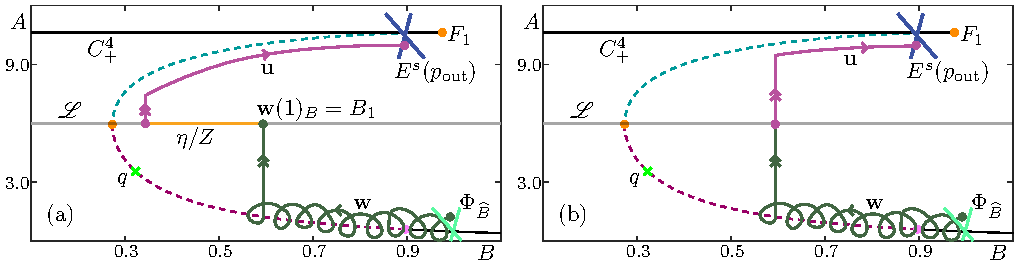
\includegraphics[]{./figures/MKMO_10.pdf}
\caption{A sketch in projection onto the $(B,A)$-plane of the numerical set-up with Lin's method for the computation of $\mathscr{H}$ to the right of $W^u(q)$.  Also shown are $C^2$, $C^3$, $C^4_\pm$, $F_1$, $F_2$, $H$, and $q$.  Panel~(a) shows a sketch at the end of the first homotopy step with $\mathbf{u} \in W^u_{L_1}$ (magenta curve)$, \mathbf{w} \in W^u_{L_2}$ (forest green curve), $\Phi_{\widehat{B}}$ from Section~\ref{sec:compWsS3}, and the Lin space $Z$ (gold line) in which the points $\mathbf{w}(1)$ and $\mathbf{u}(0)$ lie at a distance $\eta$ from each other.  Panel~(b) shows $\mathbf{w}$ and $\mathbf{u}$ after the final homotopy step at which point $\eta=0$ and $\mathbf{w}(1)=\mathbf{u}(0)$.}
\label{figure_10}
\end{figure}
%%%%%%%%%%%%%%%%%%%%%%%%%%%%%%%%%%%%%%%%%%%%%%%%%%%%%%%%%%

Figure~\ref{figure_10} illustrates, step-by-step in projection onto the $(B,A)$-plane, the homotopy steps for computing the portion of $\mathscr{H}$ to the right of $W^u(q)$.  
Each panel shows $C$ from Figure~\ref{figure_1} with $\mathscr{L} = \{ \omega \in \mathbb{R}^4 \; | \; \omega_A = 6.0 \}$ (charcoal line), $\mathbf{u} \in W^s_{\Sigma_{L_1}}$ (magenta curve), $\mathbf{w} \in W^u_{\Sigma_{L_2}}$ (forest green curve), the stable eigenspace $E^s(p_{\text{out}})$ (blue cross) from condition \eqref{specific_BC}, the two-dimensional space $\Phi_{\widehat{B}}$ (mint cross) from conditions \eqref{general_conditions_unstable_2} and \eqref{general_conditions_unstable_3}.  
In the first homotopy step, we choose $\Sigma_{L_1}=\{ \omega \in \mathbb{R}^4 \; | \; \omega_A = 6.0, \omega_Y=-1.0 \}$ and $\Sigma_{L_2}=\{ \omega \in \mathbb{R}^4 \; | \; \omega_A = 6.0, \omega_Y=3.0 \}$.  We compute $\mathbf{w}$ so that $\mathbf{w}(1)_B = B_1 = 0.6$ in the second homotopy step.  Figure~\ref{figure_10}(a) is a sketch of the numerical set-up at the end of the first homotopy step.  The points $\mathbf{w}(1)$ and $\mathbf{u}(0)$ lie in the space $Z$ (gold line) from conditions \eqref{general_conditions_heteroclinic_5} and \eqref{general_conditions_heteroclinic_6} at a distance $\eta$ from each other.  Panel~(b) is a sketch of the numerical set-up after the second homotopy step when $\mathbf{w}(1) = \mathbf{u}(0)$ and $\eta=0$.  The resulting pair $(\mathbf{w},\mathbf{u})$ satisfies conditions \eqref{general_conditions_heteroclinic_1} and \eqref{general_conditions_heteroclinic_2}--\eqref{general_conditions_heteroclinic_4} and the concatenation of $\mathbf{w}$ and $\mathbf{u}$ lies on the surface $\mathscr{H}$.

%%%%%%%%%%%%%%%%%%%%%%%%%%%%%%%%%%%%%%%%%%%%%%%%%%%%%%%%%%
\begin{figure}[t!]
\centering
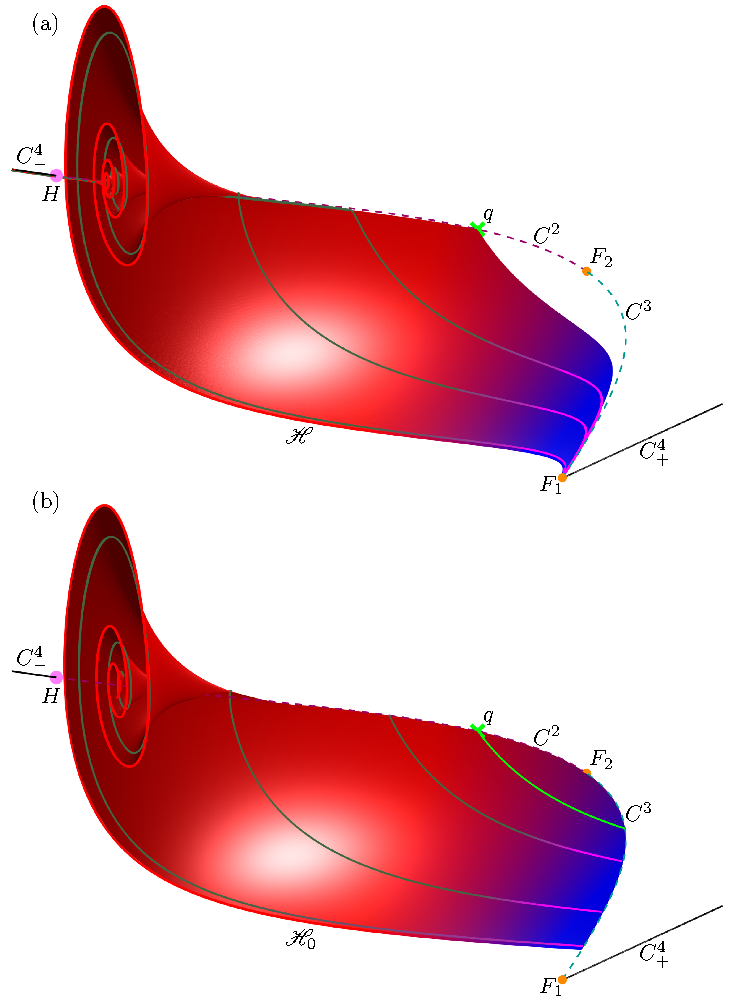
\includegraphics[]{./figures/MKMO_11.pdf}
\caption{The surface of heteroclinic connections $\mathscr{H}$ (red/blue surface) and the Lin section $\mathscr{L}$ (charcoal surface) in projection onto $(B,A,X)$-space (a) and onto $(B,A,Y)$-space (b).  The portion of $W^u(S^2)$ swept out by the family of $\mathbf{w}$ is colored red and the portion of $W^s(S^3)$ swept out by the family of $\mathbf{u}$ blue.  Also shown are representative concatenated orbit segments $(\mathbf{w},\mathbf{u})$ (forest green/magenta curves), the curves $C^2$, $C^3$, and $C^4_\pm$, and the points $F_1$, $F_2$, $H$ and $q$ which is partially obscured by $\mathscr{H}$ and $\mathscr{L}$.}
\label{figure_11}
\end{figure}
%%%%%%%%%%%%%%%%%%%%%%%%%%%%%%%%%%%%%%%%%%%%%%%%%%%%%%%%%%

After these homotopy steps, we use boundary conditions \eqref{general_conditions_heteroclinic_1} and \eqref{general_conditions_heteroclinic_2}, \eqref{general_conditions_heteroclinic_3}, \eqref{general_conditions_heteroclinic_4}, and \eqref{general_conditions_heteroclinic_5} and \eqref{general_conditions_heteroclinic_6} to sweep out a one-parameter family of paired orbit segments to obtain an accurate approximation of $\mathscr{H}$ to the right of $W^u(q)$.  Figure~\ref{figure_11} shows the computed portion of $\mathscr{H}$ (red/blue surface) with $\mathscr{L}$ (charcoal plane) in projection onto $(B,A,X)$-space in panel~ (a) and onto $(B,A,Y)$-space in panel~ (b).  Three concatenated orbit segments $(\mathbf{w},\mathbf{u})$ lying on $\mathscr{H}$ are plotted in forest green for $\mathbf{w}$ and magenta for $\mathbf{u}$.  The portion of the surface swept out by $\mathbf{w}$ is shown in red and that by $\mathbf{u}$ in blue.  Unlike other manifolds $W^s_\Sigma$ and $W^u_\Sigma$, the paired orbit segments $(\mathbf{w},\mathbf{u})$ on $\mathscr{H}$ do not contain segments that diverge quickly in the directions parallel to the $X$- and $Y$-axes.  Orbit segments lying on $\mathscr{H}$ spiral slowly around $S^2$ before crossing the surface at an intermediate speed, mostly in the direction parallel to the $A$-axis, to reach and then slowly follow $S^3$.

%%%%%%%%%%%%%%%%%%%%%%%%%%%%%%%%%%%%%%%%%%%%%%%%%%%%%%%%%%
\begin{figure}[t!]
\centering
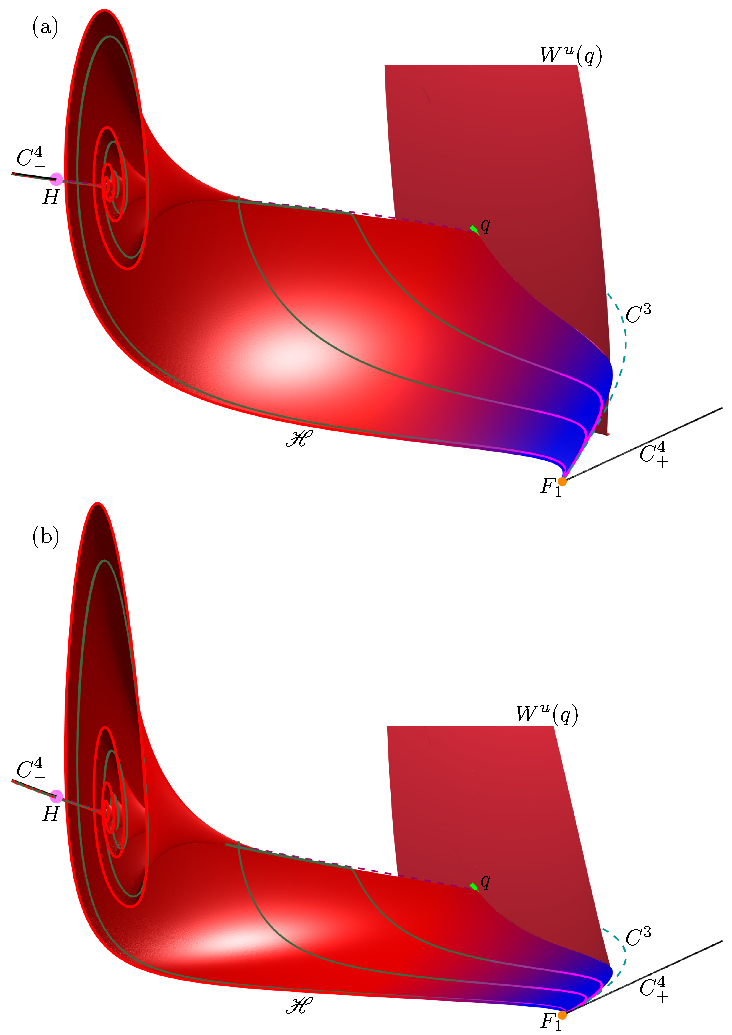
\includegraphics[]{./figures/MKMO_12.pdf}
\caption{The computed portion of $\mathscr{H}$ (red-blue fade surface) is shown in projection onto $(B,A,X)$-space (a) and onto $(B,A,Y)$-space (b) with $W^u(q)$ (cardinal surface).  The unstable manifold $W^u(q)$ bounds the computed portion of $\mathscr{H}$.  Also shown are representative concatenated orbit segments $(\mathbf{w},\mathbf{u})$ (forest green-magenta fade curves), the curves $C^2$, $C^3$, and $C^4_\pm$, and the points $F_1$, $F_2$, $H$ and $q$ which is partially obscured by $\mathscr{H}$ and $W^u(q)$.}
\label{figure_12}
\end{figure}
%%%%%%%%%%%%%%%%%%%%%%%%%%%%%%%%%%%%%%%%%%%%%%%%%%%%%%%%%%

Figure~\ref{figure_12} shows that the computed portion of $\mathscr{H}$ is bounded by $W^u(q)$ (cardinal surface); this surface was computed with the BVP approach outlined in \cite{Red_book}.  Here $\mathscr{H}$ is colored red near $S^2$ and blue near $S^3$ to illustrate that $\mathscr{H}$ is both a submanifold of $W^u(S^2)$ and of $W^s(S^3)$; compare with Figure~\ref{figure_11}.  Similarly, three concatenated orbit segments $(\mathbf{w},\mathbf{u})$ are plotted fading from forest green to magenta.  Orbits on $\mathscr{H}$ clearly follow $S^2$ on the slow time-scale, before traversing across $\mathscr{H}$ on an intermediate time-scale and then following $S^3$ on the slow time-scale.  As this figure shows, the saddle point $q$ and its two-dimensional unstable manifold $W^u(q)$ bound the computed portion of $\mathscr{H}$.  Notice how the connecting orbits nearest $W^u(q)$ follow this two-dimensional surface to come very close to $q$, before slowly following $S^2$. Hence, we computed the part of $\mathscr{H}$ to this side of $q$ as closely to $W^u(q)$ as possible.


%%%%%%%%%%%%%%%%%%%%%%%%%%%%%%%%%%%%%%%%%%%%%%%%%%%%%%%%%%
\section{Computing the surface of heteroclinic connections in the singular limit}
\label{sec:hetconn0}

We now consider the limiting surface $\mathscr{H}_0$ of connecting orbits from $C^2$ to $C^3$ for $\varepsilon = 0$.  Recall that system \eqref{equation_1} then reduces to the three-dimensional system \eqref{equation_2} in which $B$ is a parameter.  Hence, the surface $\mathscr{H}_0$ is the one-parameter family, parametrized by $B$, of connections between the saddle equilibria of \eqref{equation_2} on $C^2$ and on $C^3$, respectively.  It is simple to sweep out $\mathscr{H}_0$ with varying $B$ once an initial connection is found for fixed $B$.  The problem then reduces to finding a heteroclinic connection between two saddle equilibria in a three-dimensional system.  This is exactly the situation addressed in \cite{Lin_POs, Red_book} and we now briefly explain how this approach can be used for our purposes.

Note that we now rescale system \eqref{equation_2}, that is, we consider
%
\begin{equation}
\frac{d\mathbf{u}}{ds} = TG(\mathbf{u}),
\label{fast_rescale}
\end{equation}
%
where $\mathbf{u}(s) = (A(s), X(s), Y(s)) \in \mathbb{R}^3$ is now a three-dimensional vector, $G$ is the right-hand side of \eqref{equation_2}, and $T$ is the integration time on the fast time-scale.

We compute $\mathscr{H}_0$ as the one-parameter family of concatenated orbit segments $(\mathbf{w}, \mathbf{u})$, that are solutions of \eqref{fast_rescale}.  We again turn to Lin's method to find an initial orbit segment pair lying on $\mathscr{H}_0$ via homotopy steps.  We begin by choosing a $\widehat{B} \in (B_{\text{in}}, B_{\text{out}})$ corresponding to points $\widehat{p}_2 \in C^2$ and $\widehat{p}_3 \in C^3$.  A two-dimensional Lin section, denoted $\widehat{\mathscr{L}}$, is chosen such that, for any value of $\widehat{B} \in (B_{\text{in}}, B_{\text{out}})$, it divides the three-dimensional phase space into a region containing $\widehat{p}_2$ and a region containing $\widehat{p}_3$.  Inside $\widehat{\mathscr{L}}$, we choose a Lin vector $\mathbf{v}_Z$ with the property that it is not tangent to $W^u(\widehat{p}_2)$ or $W^s(\widehat{p}_3)$.  The Lin vector $\mathbf{v}_Z$ then defines the associated Lin space $Z$.    We then use the methods outlined in \cite{Red_book} to compute $\mathbf{w} \in W^u(\widehat{p}^2)$ and $\mathbf{u} \in W^s(\widehat{p}^3)$ satisfying appropriate boundary conditions.  We first impose two conditions,
%
\begin{equation}
	\mathbf{u}(1) \in \Upsilon^3= \{ \omega \in \mathbb{R}^3  \; | \; \left\lVert \widehat{p}_3 - \omega \right\lVert = r_3 \} \cap E^s(\widehat{p}_3),
	\label{general_conditions_heteroclinic_singular_1}
\end{equation}
%
and
%
\begin{equation}
	\mathbf{w}(0) \in \Upsilon^2= \{ \omega \in \mathbb{R}^3  \; | \; \left\lVert \widehat{p}_2 - \omega \right\lVert = r_2 \} \cap E^u(\widehat{p}_2),
	\label{general_conditions_heteroclinic_singular_2}
\end{equation}
%
where radii $r_2$ and $r_3$ are chosen such that the closed curves $\Upsilon_2$ and $\Upsilon_3$ are close to $\widehat{p}_2$ and $\widehat{p}_3$, respectively.  We next impose the conditions
%
\begin{equation}
	\mathbf{u}(0) \in \widehat{\mathscr{L}},
	\label{general_conditions_heteroclinic_singular_3}
\end{equation}
%
and
%
\begin{equation}
	\mathbf{w}(1) \in \widehat{\mathscr{L}},
	\label{general_conditions_heteroclinic_singular_4}
\end{equation}
%
while additionally requiring that
%
\begin{equation*}
	\mathbf{w}(1)-\mathbf{u}(0) \in Z.
\end{equation*}
%
As before, this can be achieved (generically) by setting
%
\begin{equation*}
	\mathbf{v}_Z = \frac{\mathbf{u}(0) - \mathbf{w}(1)}{\left\lVert \mathbf{u}(0) - \mathbf{w}(1) \right\lVert}
	\label{Lin_vector_singular}
\end{equation*}
%
for a pair $(\mathbf{w},\mathbf{u})$ of orbit segments that satisfy \eqref{general_conditions_heteroclinic_singular_3} and \eqref{general_conditions_heteroclinic_singular_4}.  The signed distance between $\mathbf{w}(0)$ and $\mathbf{u}(1)$ inside $Z$ is given by
%
\begin{equation}
	\eta = [ \mathbf{w}(0)-\mathbf{u}(1) ] \cdot \mathbf{v}_Z,
	\label{general_conditions_heteroclinic_singular_5}
\end{equation}
%
which is a regular test function.  To implement $\mathbf{u}(0), \mathbf{w}(1) \in Z$, we now define a single unit normal vector $\mathbf{n} \perp \mathbf{v}_Z$ and impose the condition
%
\begin{equation}
	[\mathbf{u}(0) - \mathbf{w}(1)] \cdot \mathbf{n} =0
	\label{general_conditions_heteroclinic_singular_7}
\end{equation}
%
which ensures that $\mathbf{w}(1)-\mathbf{u}(0)$ remains in $Z$.  Note that $\mathbf{v}_Z$ and $\mathbf{n}$ now remain fixed throughout the computation.  By construction, the pair $(\mathbf{w}, \mathbf{u})$ at the end of the first homotopy step is a solution to the 2PBVP defined by \eqref{general_conditions_heteroclinic_singular_1}, \eqref{general_conditions_heteroclinic_singular_2}, \eqref{general_conditions_heteroclinic_singular_3}, \eqref{general_conditions_heteroclinic_singular_4}, \eqref{general_conditions_heteroclinic_singular_5}, and \eqref{general_conditions_heteroclinic_singular_7}; keeping $\eta$, $T$, $\mathbf{u}(0)_B$, and $\mathbf{w}(1)_B$ as free parameters allows us to close the Lin gap and satisfy $\eta = 0$, at which point the concatenation of $\mathbf{w}$ with $\mathbf{u}$ forms a connecting orbit segment in $\mathscr{H}_0$.

In our specific set-up, we choose $\widehat{B}=0.4$, $r_3 = 0.0001$, and $\widehat{\mathscr{L}}=\{ \omega \in \mathbb{R}^4 \; | \omega_A = 6.0\; \}$.  After the above homotopy steps, we sweep out $\mathscr{H}_0$ by imposing $\eta = 0$ and increasing and decreasing the parameter $\widehat{B}$, keeping $T$, $\mathbf{w}(1)_B$, $\mathbf{u}(0)_B$, and the coordinates of $\widehat{p}_2$ and $\widehat{p}_3$ as free parameters.  Note that we are not limited by $W^u(q)$ in the computation of $\mathscr{H}_0$, because $q$ is just one of the equilibria on $C^2$.  However, there is an additional challenge due to a change in the type of equilibria on $C^2$.  For $\widehat{B} < 0.476858$, the saddle $\widehat{p}_2$ has real eigenvalues and for $\widehat{B} > 0.476858$ the eigenvalues are complex conjugate, causing spiralling of $\mathbf{w}$ that increases as $\widehat{B}$ approaches $H_B$.  More mesh points are needed to approximate $\mathbf{w}$ as this orbit segment spirals more and more.  A constant mesh size throughout the computation is an advantage when one wants to render the overall surface $\mathscr{H}_0$. Hence, we keep the mesh fixed but allow the radius $r_2$ to increase linearly from $0.0001$ to $0.2$ between $\widehat{B}=0.476858$ and $\widehat{B}=0.86$, where $p_2$ has complex-conjugate eigenvalues. Specifically, we set 
%
\[r_2= \begin{cases} 
      0.0001 & \widehat {B} < 0.476858 \\
      0.521789(\widehat{B} - 0.476858) + 0.0001 & \widehat {B} < 0.476858
   \end{cases}
\]
%
to we avoid computing tight spirals near $C^2$ that would require more mesh points and a nonconstant mesh.


%%%%%%%%%%%%%%%%%%%%%%%%%%%%%%%%%%%%%%%%%%%%%%%%%%%%%%%%%%
\begin{figure}[t!]
\centering
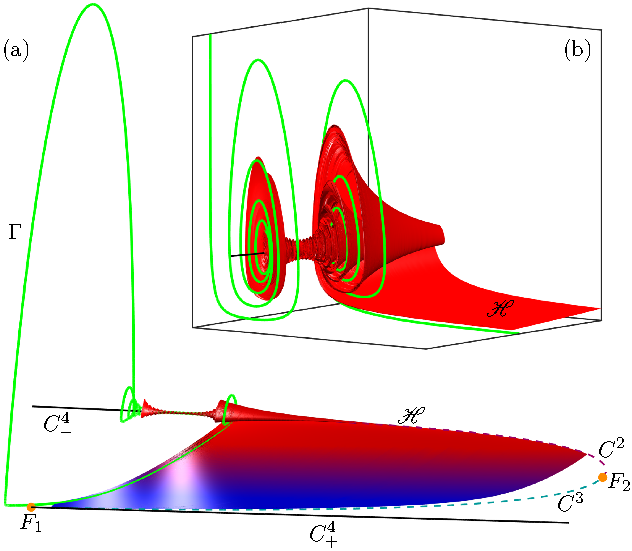
\includegraphics[]{./figures/MKMO_13.pdf}
\caption{Projections onto $(B,A,X)$-space of the portion of $\mathscr{H}_0$ lying in the region $B < 0.781$ (red-blue fade surface) (a) and of $\mathscr{H}$ for $\varepsilon=0.0037$ (red-blue fade surface) (b).   Also shown in panel~(a) for $\varepsilon=0$ are the intersection $W^u(q)\cap\mathscr{H}_0$ (green curve) for $\varepsilon=0$ and the point $p \in C^2$ (periwinkle dot) with $p_B \approx 0.477$ where the eigenvalues become complex conjugate.   Both panels also show representative orbit segments (forest green-magenta fade curves), the equilibrium $q$ (green cross), the curves $C^2$, $C^3$, and $C^4_\pm$, and the points $F_1$, $F_2$, and $H$.}
\label{figure_13}
\end{figure}
%%%%%%%%%%%%%%%%%%%%%%%%%%%%%%%%%%%%%%%%%%%%%%%%%%%%%%%%%%

Figure~\ref{figure_13} shows in projection onto $(B,A,X)$-space the two computed surfaces $\mathscr{H}_0$ for $\varepsilon=0$ (red-blue fade surface) in panel~(a) in comparison with the surface $\mathscr{H}$ for $\varepsilon=0.0037$ (red-blue fade surface) in panel~(b).  To aid a visual comparison with $\mathscr{H}$ in panel~(b), we show only the portion of $\mathscr{H}_0$ in panel~(a) that lies in the region $B < 0.781$.  Notice how $\mathscr{H}_0$ starts to spiral increasingly from the equilibrium (periwinkle dot) on $C^2$ where the eigenvalues become complex conjugate.  Due to the $B$-dependence of $r_2$, the surface does not spiral all the way into $C^3$.  In both panels, three representative orbit segments are shown on the surface (forest green-magenta fade curves).  Unlike orbit segments on $\mathscr{H}$, orbit segments on $\mathscr{H}_0$ do not exhibit any drift in the direction along $C^2$ and $C^3$, respectively because $\varepsilon=0$ so that $B$ is constant.  The intersection of $\mathscr{H}_0$ with $W^u(q)$ (green curve) for $\varepsilon=0$ is analogous to the boundary of $\mathscr{H}$ near $q$; compare with Figure~\ref{figure_12}.  The picture indicates that $\mathscr{H}$ is very close to $\mathscr{H}_0$.  We checked this observation by defining and computing an integral distance between intersection curves of $\mathscr{H}$ and $\mathscr{H}_0$ with sections where the value of $B$ is fixed; see the appendix for details.


%%%%%%%%%%%%%%%%%%%%%%%%%%%%%%%%%%%%%%%%%%%%%%%%%%%%%%%%%%
\section{Mixed-mode oscillations and their geometry}
\label{sec:mmogeom}

We now turn to the question of what role the surface of heteroclinic connections $\mathscr{H}$ plays for the geometric properties of MMOs and, especially, for the organisation of their epochs of local small-amplitude oscillations and of global large-amplitude oscillations.  

%%%%%%%%%%%%%%%%%%%%%%%%%%%%%%%%%%%%%%%%%%%%%%%%%%%%%%%%%%
\begin{figure}[t!]
\centering
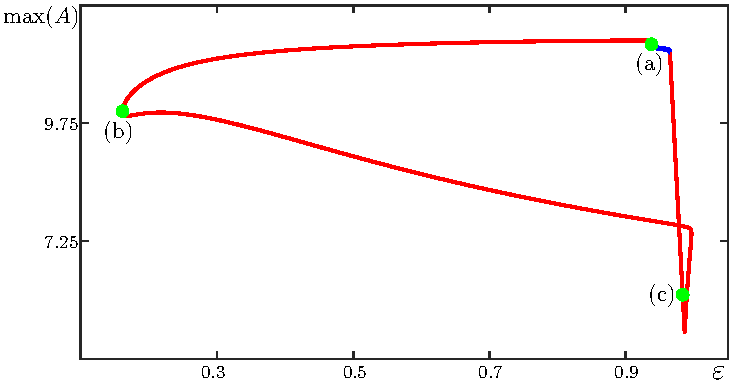
\includegraphics[]{./figures/MKMO_14.pdf}
\caption{The attracting MMO $\Gamma$ (green curve) and the surface of heteroclinic connections $\mathscr{H}$ (red-blue fade surface) for $\varepsilon=0.0037$ shown in projection onto $(B,A,X)$-space. The surface $\mathscr{H}$ is extended in backward time past the Hopf bifurcation point $H$.  Panel~(a) shows the global view of $\Gamma$ tracking $\mathscr{H}$ from $C^2$ (dashed raspberry curve) to $C^3$ (dashed teal curve) and then transitioning back to $C^4_-$ (solid black curve) which constitutes the LAO.  Panel~(b) shows an enlargement of the region where $\Gamma$ makes a subsequent slow passage past $H$ to generate SAOs.}
\label{figure_14}
\end{figure}
%%%%%%%%%%%%%%%%%%%%%%%%%%%%%%%%%%%%%%%%%%%%%%%%%%%%%%%%%%

We begin by considering the fixed value of $\varepsilon=0.0037$, for which there exists an attracting periodic orbit $\Gamma$ for $\varepsilon=0.0037$ that is clearly an MMO. Figure~\ref{figure_14} shows $\Gamma$ (green curve) in projection onto $(B,A,X)$-space with the surface $\mathscr{H}$ (red-blue fade surface) of heteroclinic connections, which has been extended in backward time past $H$.  Here the attractor $\Gamma$ was obtained by forward-time integration.  Figure~\ref{figure_14}(a) shows a global view of $\Gamma$ and $\mathscr{H}$.  We observe $\Gamma$ entering into the region of SAOs near the attracting branch $C^4_-$ of $C$.  The MMO spirals as it enters the scroll-like region of $\mathscr{H}$, with increasingly smaller SAOs as it makes a slow passage past $H$ to $C^2$; note that $S^2$ is not distinguishable from $C^2$ at this scale.  On the other side of $H$, near $C^2$, we observe the SAOs increasing in size until $\Gamma$ leaves the region of SAOs.  An enlargement of the slow passage near $H$ is shown in panel~(b).  In this enlargement, we also see $\Gamma$ exit the region of SAOs by spiralling out of the scrolls of $\mathscr{H}$ to the underside of the flatter part of $\mathscr{H}$ in between $C^2$ and $C^3$.  The global view in Figure~\ref{figure_14}~(a) shows that $\Gamma$ subsequently tracks an orbit segment on $\mathscr{H}$ at an intermediate speed to cross over to $C^3$; again, $S^3$ is not distinguishable from $C^3$ at this scale.  We find that $\Gamma$ extends slightly past the fold point $F_1$ before making a single LAO, mostly in the $X$- and $Y$-directions, back to the attracting slow manifold near $C^4_-$.  Hence, we conclude that the global return mechanism of $\Gamma$, from a region of SAOs via an LAO and back to the region of SAOs, clearly involves the surface of heteroclinic connections $\mathscr{H}$.

%%%%%%%%%%%%%%%%%%%%%%%%%%%%%%%%%%%%%%%%%%%%%%%%%%%%%%%%%%
\begin{figure}[t!]
\centering
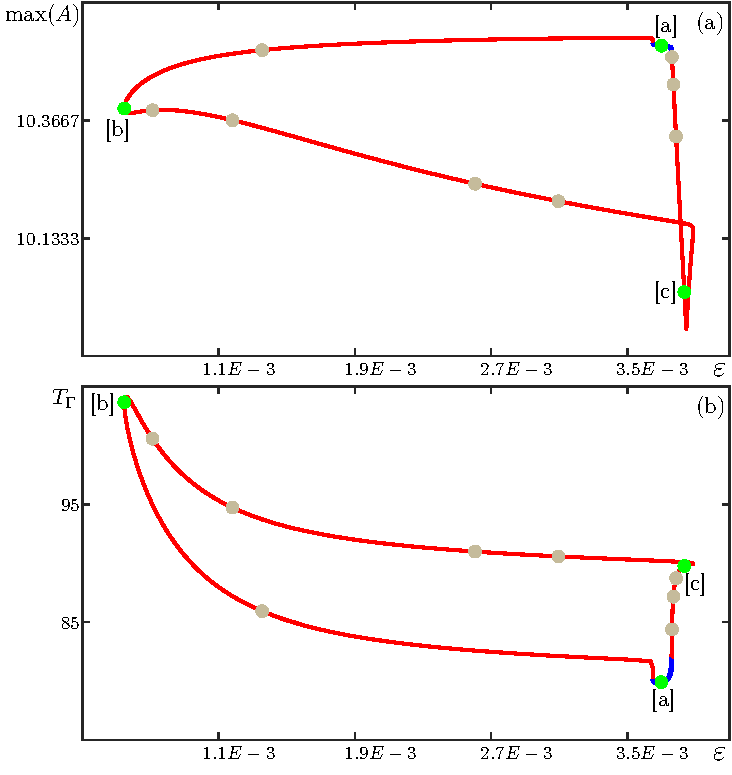
\includegraphics[]{./figures/MKMO_15.pdf}
\caption{Isola of periodic MMOs $\Gamma$ when $\varepsilon$ is varied, shown in terms of the maximum value of $A$ (a) and its period $T_\Gamma$ (b), respectively.  Here, $\Gamma$ is stable along the blue part and unstable along the red part of the isola.  Green dots labeled [a], [b], and [c] correspond to $\Gamma$ as shown in Figure~\ref{figure_16}; these and the taupe dots correspond to MMOs shown in Figures~\ref{figure_17} and~\ref{figure_18}.}
\label{figure_15}
\end{figure}
%%%%%%%%%%%%%%%%%%%%%%%%%%%%%%%%%%%%%%%%%%%%%%%%%%%%%%%%%%

Singular objects generally play a role in organizing the geometry of an MMO provided $\varepsilon$ is small enough; see \cite{MMO} for an overview and original references.  Indeed, any periodic MMOs can be continued for decreasing $\varepsilon$, ideally to their singular limits for $\varepsilon=0$ to connect with theoretical results \cite{Nonlinearity, MMO, Autocatalator}.  This motivates us to investigate the MMO periodic orbit $\Gamma$ for varying $\varepsilon$. Figure~\ref{figure_15} shows that the continuation of $\Gamma$ in $\varepsilon$ results in an isola; that is, a closed curve when an observable is plotted against $\varepsilon$. Here we show as observables the maximum $A$-value along $\Gamma$ in panel~(a) and the period $T_\Gamma$ of $\Gamma$ in panel~(b). Here, the short blue segment of the isola indicates where $\Gamma$ is stable; it is unstable along the red segment, meaning that $\Gamma$ has at least one unstable Floquet multiplier. It is known from previous literature that MMO periodic orbits may form isolas when other parameters are varied \cite{Nonlinearity, Forest_pest_model}.  Specifically for the Olsen model, isolas were found in \cite{QSSA} where a single parameter in their formulation was changed; in our context this would mean changing $\alpha$, $\varepsilon$, $\kappa$, and $\lambda$ simultaneously in a certain way; see \cite{Rescaling} for the exact parameter rescalings. Nevertheless, it is somewhat surprising that we find that $\Gamma$ forms an isola when continued in $\varepsilon$. In particular, the continuation of $\Gamma$ does not reach $\varepsilon=0$. Rather there is a minimum at the fold point for $\varepsilon \approx 0.00055$, and also a maximum at another fold point for $\varepsilon \approx 0.00389$; hence, the MMO periodic orbit $\Gamma$ exists only for this range of $\varepsilon$.  

The question arises how $\Gamma$ changes during one loop around the isola and whether its (changing) geometric properties can be related to singular objects for $\varepsilon=0$. In Figure~\ref{figure_15} the green dot labeled [a] corresponds to the original stable MMO shown in Figure~\ref{figure_14}. More dots are shown along the isola, and they correspond to MMOs that are shown and discussed in the remainder of this section. First of all, there are two more labeled dots: the green dot labeled [b] at the minimum in $\varepsilon$ and the green dot labeled [c], which is chosen such that the corresponding MMO is representative of a particularly interesting geometry of $\Gamma$. The MMO periodic orbits at these green dots [a]-[c] are shown in Figure~\ref{figure_16} together with $\mathscr{H}_0$ and other singular objects introduced below.  Moreover, Figure~\ref{figure_17} shows projections onto the $(B,A)$-plane of $\Gamma$ and the singular objects at the green dots [a]-[c], as well as at the intermediate taupe dots along the isola in Figure~\ref{figure_15}; the corresponding time traces of the $X$-coordinate of these MMO periodic orbits are shown in Figure~\ref{figure_18}.

%%%%%%%%%%%%%%%%%%%%%%%%%%%%%%%%%%%%%%%%%%%%%%%%%%%%%%%%%%
\begin{figure}[t!]
\centering
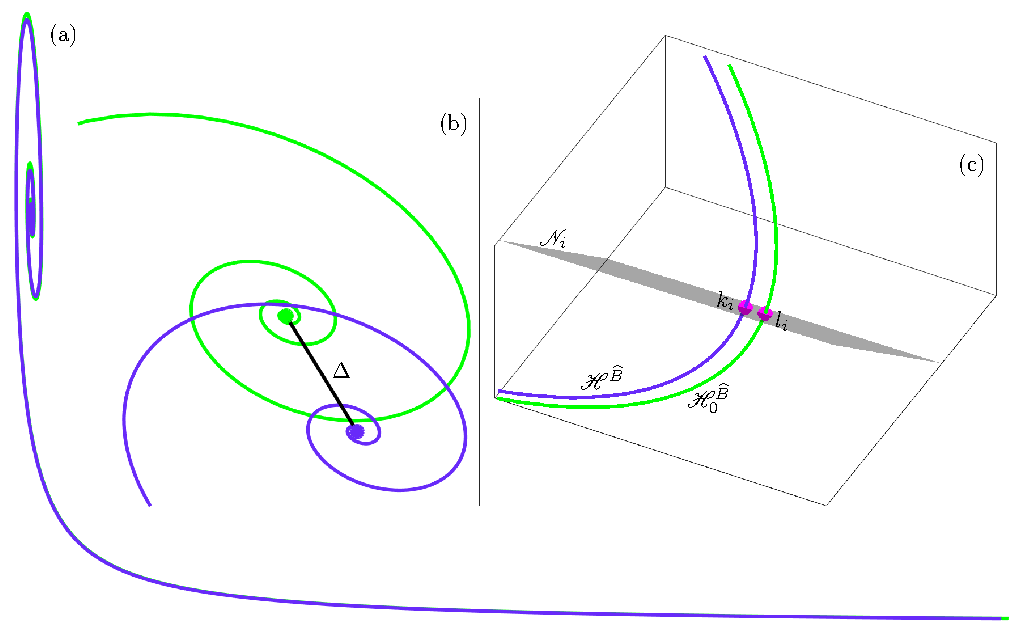
\includegraphics[]{./figures/MKMO_16.pdf}
\caption{The periodic MMO $\Gamma$ (green curve) shown in projection onto $(B,A,X)$-space with the portion of $\mathscr{H}_0$ (red-blue fade surface) lying in the region $B<0.781$, the jump-back trajectory $\mathscr{J}$ (magenta curve) and its dual $\mathscr{J}^*$ (magenta curve), and the surface $\mathscr{P}$ of singular periodic orbits (midnight-grape surface).  Also shown are $C^2$, $C^3$, $C^4_\pm$, $F_1$, $F_2$, and $H$.  Panel~(a) shows $\Gamma$ for the orignal value of $\varepsilon=0.0037$ and panels~(b) and~(c) show $\Gamma$ for $\varepsilon=0.00055$ and $\varepsilon=0.00383$ at the points labeled [b] and [c] in Figure~\ref{figure_15}, respectively.}
\label{figure_16}
\end{figure}
%%%%%%%%%%%%%%%%%%%%%%%%%%%%%%%%%%%%%%%%%%%%%%%%%%%%%%%%%%

Figure~\ref{figure_16} shows $\Gamma$ in projection onto $(B,A,X)$-space for three values of $\varepsilon$ in relation to several singular objects of the limit $\varepsilon = 0$.  Specifically, we show portions of $C^2$, $C^3$, $C^4_\pm$, $\mathscr{H}_0$, and three additional singular objects.  The singular jump orbit $\mathscr{J}$ (magenta curve) is the solution of the reduced system \eqref{equation_2} that connects the point $F_1$ to the branch $C^4_-$; indeed, the corresponding point on $C^4_-$ is the only attractor for this value of $B$.  The dual of $\mathscr{J}$, denoted $\mathscr{J}^*$ (magenta curve), is a trajectory on $\mathscr{H}_0$ that lies at an equal distance away from $H$ in the $B$-direction.  We refer to $\mathscr{J}^*$ as the dual of $\mathscr{J}$ because, in the limit of $\varepsilon = 0$, the drift in $B$ along $C^4_-$ from $\mathscr{J}$ to $H$ takes the same time as the drift in $B$ along $C^2$ from $H$ to $\mathscr{J}^*$.  A surface $\mathscr{P}$ of singular saddle periodic orbits (midnight-grape surface) originates from $H$ and ends at a homoclinic connection to an equilibrium on $C^3$.  Each periodic orbit for fixed $B$ on the surface $\mathscr{P}$ has a two-dimensional stable and a two-dimensional unstable manifold.  Hence, the surface $\mathscr{P}$ has a three-dimensional stable and unstable manifolds.

Figure~\ref{figure_16}(a) shows the attracting MMO $\Gamma$ for the original value of $\varepsilon=0.0037$, the same as in Figure~\ref{figure_14} and corresponding to the green dot labeled [a] in Figure~\ref{figure_15}.  As in Figure~\ref{figure_14}, $\Gamma$ is seen to enter into the region of SAOs near the attracting branch $C^4_-$ of $C$ exhibiting decreasing SAOs as it spirals through the surface $\mathscr{P}$ of singular periodic orbits. The SAOs increase as $\Gamma$ passes $\mathscr{P}$ near the Hopf point $H$.  Then $\Gamma$ exits the region of SAOs by following $\mathscr{H}_0$ closely to a region near $C^3$ (illustrating again the closeness of $\mathscr{H}_0$ and $\mathscr{H}$ at this scale).  It extends past $F_1$ before making an LAO back to $C^4_-$.  The single LAO somewhat tracks the singular jump orbit $\mathscr{J}$ (magenta curve) from $F_1$ to $C^4_-$.  We also observe that $\Gamma$ exits the region of SAOs near its dual $\mathscr{J}^*$ (magenta curve).  These observations are consistent with our expectation that the SAOs are due to the tourbillon mechanism of passage through a Hopf bifurcation as described in \cite{MMO}; in particular, the distance between $H$ and where $\Gamma$ enters the region of SAOs is similar to the distance between $H$ and where $\Gamma$ leaves it.  This also means that the number of SAOs exhibited by $\Gamma$ before reaching $H$ is approximately the same as the number of SAOs exhibited after passing it.  Overall, Figure~\ref{figure_16}(a) suggests that $\mathscr{J}$, $\mathscr{J}^*$, and appropriate portions of $C^2$, $C^3$, $C^4_\pm$, and $\mathscr{H}_0$ may act as a singular limit for $\Gamma$.

Figure~\ref{figure_16}(b) shows $\Gamma$ for the smaller value of $\varepsilon=0.00055$, corresponding to the green dot labeled [b] at the minimum of the isola in Figure~\ref{figure_15}.  We see $\Gamma$ entering the region of SAOs via the attracting branch $C^4_-$.  The periodic orbit $\Gamma$ now closely follows the surface of singular periodic orbits $\mathscr{P}$ generating large SAOs in the process.  Notice that $\Gamma$ does not pass near $H$, but passes through $\mathscr{P}$ in the $(B,A,X)$-projection.  The MMO then follows the two-dimensional intersection of $W^s(C^3)$ and the unstable manifold of $\mathscr{P}$ (not shown) away from $\mathscr{P}$ toward $C^3$.  As the MMO crosses the region between $C^4_-$ and $C^3$, it exhibits minimal drift in the $B$-direction due to the smaller value of $\varepsilon$, compare with panel~(a).  Almost immediately after reaching $C^3$, $\Gamma$ makes an LAO that tracks the singular homoclinic connection which limits the surface $\mathscr{P}$, back to the region of SAOs.  The MMO shown in Figure~\ref{figure_16}(b) features a much narrower range of $B$-values than the one shown in panel~(a) while the amplitude of the SAOs is larger.  Our observations in panel~(b) suggest that $\Gamma$ has $\mathscr{P}$ as a singular limit, which corresponds to a much more localized phenomenon.

Figure~\ref{figure_16}(c) shows $\Gamma$ for the larger value of $\varepsilon=0.00383$, corresponding to the green dot labeled [c] in Figure~\ref{figure_15}.  As in Figure~\ref{figure_16}(a), $\Gamma$ enters the region of SAOs near where $\mathscr{J}$ meets $C^4_-$, transitions through $H$ to $C^2$, exits the region of SAOs near $\mathscr{J}^*$, and follows $\mathscr{H}_0$ to $C^3$.  Upon reaching $C^3$ well before $F_1$, the MMO $\Gamma$ has an LAO that quickly takes it back to $C^2$ rather than to $C^4_-$.  Without exhibiting any SAOs, it then drifts back to $C^3$ and has a second LAO starting well past $F_1$, very much like the LAO of the MMO in panel~(a).  For this MMO appears to be quite different qualitatively, featuring two LAOs, and it is unclear what role the different singular objects play in this.

%%%%%%%%%%%%%%%%%%%%%%%%%%%%%%%%%%%%%%%%%%%%%%%%%%%%%%%%%%
\begin{figure}[t!]
\centering
%% 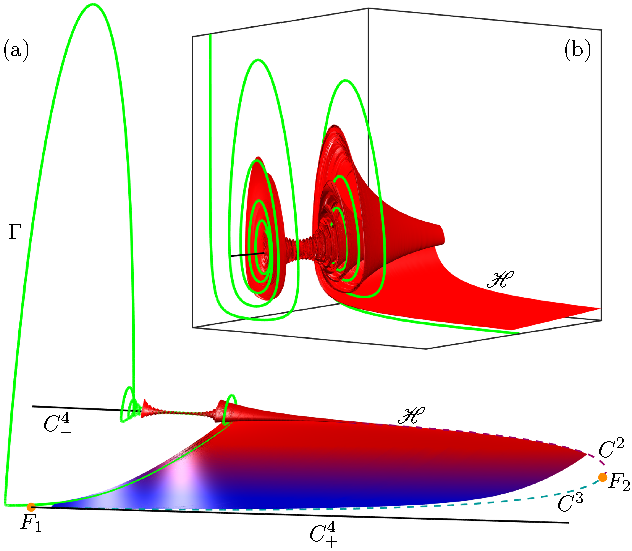
\includegraphics[]{./figures/MKMO_17.pdf}
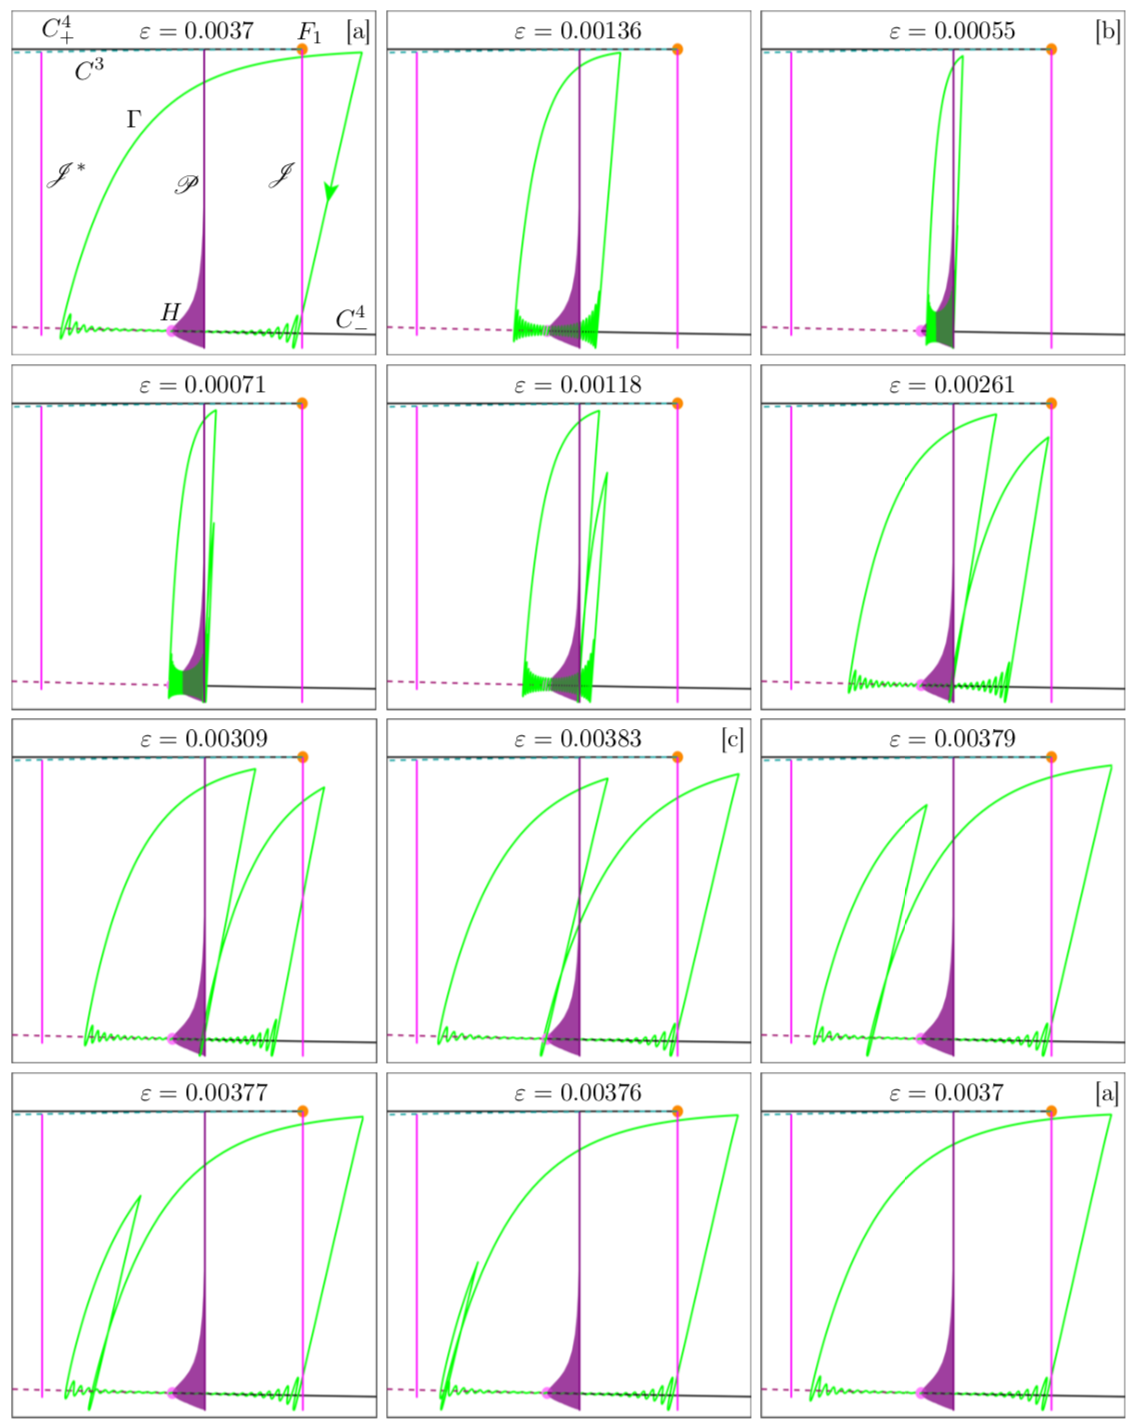
\includegraphics[width=17.4cm]{./figures/MKMO_17_scan.png}
\caption{Projections onto the $(B,A)$-plane of the MMO $\Gamma$ (green curve) showing its evolution when varying $\varepsilon$ counter-clockwise around the isola in Figure~\ref{figure_15}.  Panels with labels [a], [b], and [c], and those without labels correspond to the labeled and taupe dots in Figure~\ref{figure_15}, respectively; compare also with Figure~\ref{figure_16}.  Also shown are $\mathscr{J}$ and $\mathscr{J}^*$ , $\mathscr{P}$, $F_1$, $H$, and segments of $C^2$, $C^3$, and $C^4_\pm$; see their labels in the first panel.}
\label{figure_17}
\end{figure}
%%%%%%%%%%%%%%%%%%%%%%%%%%%%%%%%%%%%%%%%%%%%%%%%%%%%%%%%%%

%%%%%%%%%%%%%%%%%%%%%%%%%%%%%%%%%%%%%%%%%%%%%%%%%%%%%%%%%%
\begin{figure}[t!]
\centering
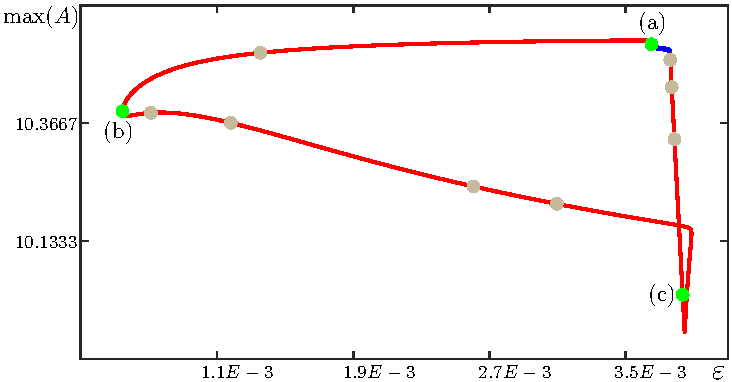
\includegraphics[]{./figures/MKMO_18.pdf}
\caption{Time series of the $X$-coordinate of the periodic MMO $\Gamma$ over one period $T_\Gamma$ (shown at top of panels) for varying $\varepsilon$; the individual panels correspond directly to those of Figure~\ref{figure_17}.}
\label{figure_18}
\end{figure}
%%%%%%%%%%%%%%%%%%%%%%%%%%%%%%%%%%%%%%%%%%%%%%%%%%%%%%%%%%

%%% NOTE: figures here and cleared to ensure proper positioning in text
\clearpage

Figure~\ref{figure_16} illustrates that the behavior of $\Gamma$ changes significantly around the isola.  A natural question is then how $\Gamma$ deforms continuously as one moves around the isola.  The change in geometry is shown in finer detail in the panels of Figure~\ref{figure_17}. This figure can be imagined as stills of an animation, beginning and ending at the original MMO for $\varepsilon=0.0037$, as the isola is followed in a counter-clockwise direction, where the individual images are taken at the marked dots in Figure~\ref{figure_15}. In Figure~\ref{figure_17} we show the projection onto the $(B,A)$-plane of $\Gamma$ and also the singular objects $\mathscr{J}$, $\mathscr{J}^*$, $\mathscr{P}$, $F_1$, $H$, and relevant portions of $C$.  The MMO periodic orbits shown in the panels labeled [a], [b], and [c] correspond to the instances of $\Gamma$ shown in Figure~\ref{figure_16}(a), (b), and (c); the other panels are for the the intermediate unlabeled taupe dots in Figure~\ref{figure_15}; in each panel of Figure~\ref{figure_17} the corresponding value of $\varepsilon$ is shown at the top. Figure~\ref{figure_18} shows the time series of the $X$-coordinate over one period of the MMO $\Gamma$ along the isola for the exact same values of $\varepsilon$, again imagined as stills of an animation.  Here, the horizontal axis is the rescaled time variable $t \in [0,1]$, and the period $T_\Gamma$ of the periodic MMO is shown at the top of each panel with the corresponding value of $\varepsilon$.

The first row of panels in Figures~\ref{figure_17} and~\ref{figure_18} illustrates the transition of $\Gamma$ from $\varepsilon=0.0037$ at [a] to $\varepsilon=0.00055$ at [b].  Note in Figure~\ref{figure_17} how the $B$-direction narrows continuously and the amplitude of SAOs increases.  In the process, $\Gamma$ makes an earlier fast exit from the region of $C^3$, well before reaching the point $F_1$.  The intermediate panel is a good example of a tourbillon mechanism with a nearly symmetrical change in sufficiently large amplitude of the SAOs on either side of $H$.  As a result, the periodic MMO $\Gamma$ for $\varepsilon=0.00055$ at [b] is quite localized near the point $H$; compare with Figure~\ref{figure_16}(b) and note that $\Gamma$ lies entirely to one side of $H$.  The corresponding panels in Figure~\ref{figure_18} clearly illustrate the increasing amplitude of SAOs; notice also the increasing period of SAOs as $\varepsilon$ decreases.

The subsequent transition from [b] to [c] is shown in Figures~\ref{figure_17} and~\ref{figure_18} in the second row and up to the middle panel of the third row.  The main feature is that the outermost SAO increases in amplitude to become a second LAO.  Already for $\varepsilon=0.00071$, the largest SAO immediately after the LAO has increased so much in amplitude that we refer to it as an LAO.  This is seen even more clearly in Figure~\ref{figure_18}, where there is a clear gap in the time series between LAOs.  As $\varepsilon$ is increased further, to $\varepsilon=0.00118$, this panel looks like the panel directly above it with an additional LAO on the left.  The first LAO back to $C^4_-$ is initially to the right of $H$ in Figure~\ref{figure_17}, but it moves left as $\varepsilon$ is increased and the first LAO occurs earlier and earlier until it is approximately at $H$ in panel~[c].  Corresponding panels in Figure~\ref{figure_18} show that the distance between the two LAOs increases and the tourbillon mechanism becomes smaller in amplitude.

The remaining panels of Figures~\ref{figure_17} and~\ref{figure_18} show the transition from [c] back to [a].  The tourbillon mechanism does not change in these panels, the only change we observe is an increasing gap between the first and second LAO until the distance between the last SAO and the first LAO is much smaller than the distance between LAOs.  In this process, the amplitude of the first LAO decreases substantially until it is of the same order of magnitude as the last SAO, and so we refer to it again as an SAO.  This increase in the distance between LAOs corresponds, in Figure~\ref{figure_17}, to the the first return to $C^4_-$ after the SAOs moving well to the left of $H$.  We can see the decrease of the maximum $A$-value in Figure~\ref{figure_17} for the first, left-most LAO until we return to the periodic MMO $\Gamma$ back at [a].  A similar decrease of the $X$-coordinate can be observed in the corresponding panels of Figure~\ref{figure_18}.

Overall, we conclude that the periodic MMO periodic orbit $\Gamma$ changes considerably along the $\varepsilon$-isola in the following way: SAOs grow and then shrink in amplitude, generating a second LAO in the process that splits on one side and then rejoins on the other.  Moreover, we see that the singular objects that appear to be influencing the geometry of MMOs change as $\Gamma$ makes its way around the isola.  For the original value $\varepsilon=0.0037$, as well as other relatively large values of $\varepsilon$, the singular jump orbits $\mathscr{J}$ and $\mathscr{J}^*$ appear to limit the tourbillon mechnisms of generating SAO via a close passage near the singular Hopf bifurcation point $H$. For $\varepsilon=0.00055$ and other relatively small values of $\varepsilon$, on the other hand, we find that the singular surface $\mathscr{P}$ plays a role for the return mechanism of the second LAO. Along the entire isola, the surface $\mathscr{H}$ of heteroclinic connections and its singular limit $\mathscr{H}_0$ are the objects that enable the global exit of $\Gamma$ from a region of SAOs and the generation of a subsequent LAO. We conclude that the surface $\mathscr{H}$ of heteroclinic connections between two one-dimensional saddle branches of the slow manifold is an integral geometric ingredient of a previously unknown mechanism for the generation of MMOs in a four-dimensional phase space.


%%%%%%%%%%%%%%%%%%%%%%%%%%%%%%%%%%%%%%%%%%%%%%%%%%%%%%%%%%
\section{Conclusions and outlook}
\label{sec:concl}

We studied a four-dimensional model of peroxidase-oxidase reaction due to Olsen~[1983], in a parameter regime where one variable is slow and three variables are fast~\cite{Rescaling}. The basic underlying invariant set in the singular limit is a one-dimensional S-shaped critical manifold consisting of equilibria of different stability types. One branch is stable and connects at a fold point to a saddle branch, which subsequently connects at a second fold point to another branch of saddle equilibria. Hence, there exist two branches of saddle equilibria with different indices (number of unstable directions). When $\varepsilon$ is increased from $\varepsilon = 0$, these two branches of equilibria perturb to one-dimensional slow manifolds of the full system --- one with a three-dimensional stable manifold and the other with a three-dimensional unstable manifold. Therefore, there is the possibility that these two manifolds intersect and, if they do, they intersect generically in a surface of connecting orbits.

We presented a numerical set-up to compute the objects involved, specifically: \\[-6mm]
%
\begin{list}{(\roman{enumi})}{\usecounter{enumi}
    \setlength{\leftmargin}{9mm} \setlength{\labelwidth}{9mm} \setlength{\itemsep}{0mm}}
\item
one-dimensional saddle slow manifolds in a four-dimensional phase space; \\[-4mm]
\item
two-dimensional submanifolds of their three-dimensional (un)stable manifolds; and \\[-4mm]
\item
a surface of connecting orbits from one slow manifold to the other. \\[-5mm]
\end{list}
%
The underlying idea is to represent each of these objects as (families of) orbit segments that are solutions of suitably defined boundary value problems; the latter are then solved by a boundary value problem solver in conjunction with numerical continuation, and we used the package \textsc{AUTO} for this task. More specifically, we computed a one-dimensional saddle slow manifold as an orbit segment that stays for the longest time in a tubular neighborhood of the respective branch of equilibria of the critical manifold. Subsequently, we computed pieces of two-dimensional stable or unstable submanifolds as families of orbit segments that start or end in a suitable section further away and then enter and stay in the tubular neighborhood for an order-one amount of time on the slow time scale. This is a generalization to a four-dimensional setting of the approach from \cite{Saeed_Paper} for systems with one slow and two fast variables; as a new element, we defined several three-dimensional and two-dimensional sections to which the end points of orbit segments are restriced during the different steps of such a computation. To find connecting orbits we employed a Lin's method approach: we considered a pair of orbit segments, one in the three-dimensional stable manifold of one slow manifold and a second in the three-dimensional unstable manifold of the other slow manifold, with one end point each in a common three-dimensional section. The signed distance along a fixed direction of the two end points is (generically) a well-defined test function for the occurrence of a connecting orbit. We found a first connecting orbit as a zero of this test function, and then swept out the surface of connections in a subsequent continuation run.

Our computations showed that there is indeed a surface $\mathscr{H} = W^s(S^2) \cap W^u(S^3)$ of connecting orbits between two saddle slow manifold $S^2$ and $S^3$; specifically, we computed $\mathscr{H}$ for $\varepsilon = 0.0037$. This confirmed a suggestion in \cite{QSSA}, based on a quasi steady-state assumption, that such a connection may exist in the four-dimensional Olsen model. Even though our choice of parameters for the Olsen model places it in the class of systems with three fast variables according to \cite{Rescaling}, orbits on the surface $\mathscr{H}$ evolve on an intermediate time-scale. Namely, we find that the variable $A$, while definitely faster than the slow variable $B$, evolves considerably slower on $\mathscr{H}$ than both $X$ and $Y$. In other words, finding $\mathscr{H}$ reveals an intermediate time-scale in the region of phase space where this surface exists. This is the case because connecting orbits on $\mathscr{H}$ approach both $S^2$ and $S^3$ tangent to the eigenspaces of the respective weakest stable and unstable eigenvalues, which are the eigenvalues that become zero at the fold point where $S^2$ and $S^3$ meet. Which of the fast variables, or which combination thereof, experiences the associated slowing-down depends on the components of the weakest eigendirections in the fast subspace. 

We next showed that the surface $\mathscr{H}$ plays a crucial part in the global reinjection mechanism of a stable MMO (mixed-mode oscillation) periodic orbit $\Gamma$, which features a single LAO (large-amplitude oscillation) and SAOs (small-amplitude oscillations) that are generated by a passage near the (singular) Hopf bifurcation point. Following an orbit on $\mathscr{H}$ closely allows $\Gamma$ to make a transition (at an intermediate time-scale) from one saddle slow manifold in the region of SAOs past the Hopf bifurcation to the other slow manifold, which it then follows slowly to a fold point where a very fast transition segment is responsible for the return back to the region of SAOs. Continuation of the MMO periodic orbit in $\varepsilon$ towards the singular limit $\varepsilon = 0$ revealed that $\Gamma$ lies on an isola, that is, it exists only for a finite interval of $\varepsilon$-values that come close to but do not reach $\varepsilon = 0$. When followed once around the isola, $\Gamma$ was found to change quite dramatically: the first SAO grows and becomes another LAO; subsequently, the original LAO shrinks to become the last SAO. We illustrated this by showing representative instances of $\Gamma$ along the isola together with the singular objects for $\varepsilon = 0$, including the surface $\mathscr{H}_0 = W^s(C^2) \cap W^u(C^3)$ of connecting orbits between the corresponding equilibrium branches $C^3$ to $C^2$ of the critical manifold. We computed $\mathscr{H}_0$ also with a Lin's method approach and checked that $\mathscr{H}$ for $\varepsilon = 0.0037$ is very close to $\mathscr{H}_0$, as theory predicts. 

Our numerical set-up for the computation of one-dimensional slow manifolds and their (un)stable manifolds nicely complements the methods from \cite{Cris_paper} for the computation of two-dimensional slow manifolds and their (un)stable manifolds. Hence, there now exists a suite of advanced numerical tools that can be used for the bifurcation analysis of slow-fast systems with phase spaces of dimension four (or even larger). Many systems, such as the Olsen model, have a explicit time-scale separation into different groups of variables. On the other hand, for many systems arising in applications this is not the case and their slow-fast nature depends on where in phase space a trajectory, or a segment of a trajectory, lies; in particular, slow manifolds in different parts of phase space may have different dimensions. Our boundary value problem formulations do not require an explicit time-scale separation, and the same is true for the related numerical methods in \cite{homotopy_example, Cris_paper,Saeed_Paper, Jose_Paper}. Rather, what is needed is local stability information near different parts of critical manifold. It is an interesting subject for future research to couple these methods for the computation of slow manifolds of different dimensions with numerical methods that are able to determine an only implicitly given slow-fast structure~\cite{Lizarraga_paper, Wechselberger_book}, thus, providing the necessary information about local critical manifolds.

Regarding the Olsen model itself, there are certainly a number of interesting open question concerning the organization of its MMOs. The fact that the isola of MMO periodic orbits $\Gamma$ does not reach the singular limit is intriguing, because it raises the question what singular limit one should consider. Answering this question, which is the subject of ongoing research, may well require varying other system parameters. In particular, we are investigating the influence of the relative time-scale difference between $A$ and $B$ on the MMO geometry that we find along the isola. Another direction for future research is to consider the Olsen model in the same spirit for different ranges of its system parameters. 

The arrangement of singular objects responsible for the existence of the surface $\mathscr{H}$, namely a folding one-dimensional critical manifold with two saddle branches, is not exclusive to the Olsen model but generic. This means that a surface $\mathscr{H}$ of connecting orbits between two saddle-slow manifolds must be expected to be present in any other slow-fast systems with one slow and three fast variables and a folded saddle critical manifold. In fact, the entire mechanism that gives rise to the types of MMOs found in the Olsen model may also exist in other four-dimensional slow-fast systems. On the other hand, a surface such as $\mathscr{H}$ can also exist in conjunction with other (arrangements of) invariant objects of the singular limit. It will be interesting to study what types of global dynamics, and possibly associated MMOs, may be generated in this way in other slow-fast systems. 


\bigskip

%%%%%%%%%%%%%%%%%%%%%%%%%%%%%%%%%%%%%%%%%%%%%%%%%%%%%%%%%%
\section*{Acknowledgments}
%
The authors thank John Guckenheimer, Ian Lizarraga and Martin Wechselberger for fruitful discussions. This research was supported by Royal Society Te Ap\={a}rangi Marsden Fund grant \#16-UOA-286. 


\newpage

%%%%%%%%%%%%%%%%%%%%%%%%%%%%%%%%%%%%%%%%%%%%%%%%%%%%%%%%%%

\appendix{Computing the Distance of $\mathscr{H}$ from $\mathscr{H}_0$}
\label{sec:dist}
%
Fenichel theory implies that $\mathscr{H}$ converges to $\mathscr{H}_0$ with decreasing $\varepsilon$ \cite{Fenichel}.  A natural question is then how close $\mathscr{H}_0$ and $\mathscr{H}$ are to each other for $\varepsilon=0.0037$.  To investigate the distance of $\mathscr{H}$ from $\mathscr{H}_0$, we stratify the surfaces into intersections with sections $\Lambda = \{ \omega \in \mathbb{R}^4 \; | \; \omega_B = \widehat{B}\}$ for several values of $\widehat{B}$.  We denote intersections $\mathscr{H} \cap \Lambda := \mathscr{H}^{\widehat{B}}$ and $\mathscr{H}_0 \cap \Lambda := \mathscr{H}_0^{\widehat{B}}$, respectively.  A $\widehat{B}$-dependent integral distance between $\mathscr{H}^{\widehat{B}}$ and $\mathscr{H}_0^{\widehat{B}}$ in $\Lambda$ can then be computed to give an idea of the distance of $\mathscr{H}$ from $\mathscr{H}_0$.

Any $\mathscr{H}_0^{\widehat{B}}$ can readily be obtained by including the requirement that $B=\widehat{B}$ in the computation of $\mathscr{H}_0$.  We increase the mesh size for accuracy in the computation and take $r_2=1\times10^{-3}$.  Since we do not intend to render a surface after the computation of $\mathscr{H}_0^{\widehat{B}}$, it is not necessary here to keep the mesh size constant for all $\widehat{B}$.

To compute $\mathscr{H}^{\widehat{B}}$, we could use a computer package such as $\textsc{Matlab}$ to approximate the intersection curve $\mathscr{H}^{\widehat{B}} = \mathscr{H} \cap \Lambda$ from the data of the computed surface $\mathscr{H}$.  However it is much more accurate and elegant to compute $\mathscr{H}^{\widehat{B}}$ via continuation, which works as follows.  We first follow the steps for computing $\mathscr{H}$ and stop the continuation when $\mathbf{u}(0)_B = \widehat{B}$ instead of sweeping out the entire surface.  We then replace conditions \eqref{general_conditions_heteroclinic_1} and \eqref{general_conditions_heteroclinic_2} with the new boundary conditions
%
\begin{equation}
	\mathbf{u}(0) \in \Lambda
	\label{general_conditions_intersection_1}
\end{equation}
%
and
%
\begin{equation}
	\mathbf{w}(0) \in \Lambda
	\label{general_conditions_intersection_2}
\end{equation}	
%
and continue the one-parameter family of paired orbit segments $(\mathbf{w},\mathbf{u})$ satisfying \eqref{general_conditions_heteroclinic_3}, \eqref{general_conditions_heteroclinic_4}, \eqref{general_conditions_heteroclinic_5}, \eqref{general_conditions_heteroclinic_6}, \eqref{general_conditions_intersection_1}, and \eqref{general_conditions_intersection_2} with varying $\mathbf{u}(0)_A$ and $T$.  The curve $\mathscr{H}^{\widehat{B}}$ is then given as the one-parameter family $\mathbf{u}(0)$.

%%%%%%%%%%%%%%%%%%%%%%%%%%%%%%%%%%%%%%%%%%%%%%%%%%%%%%%%%%
\begin{figure}[t!]
\centering
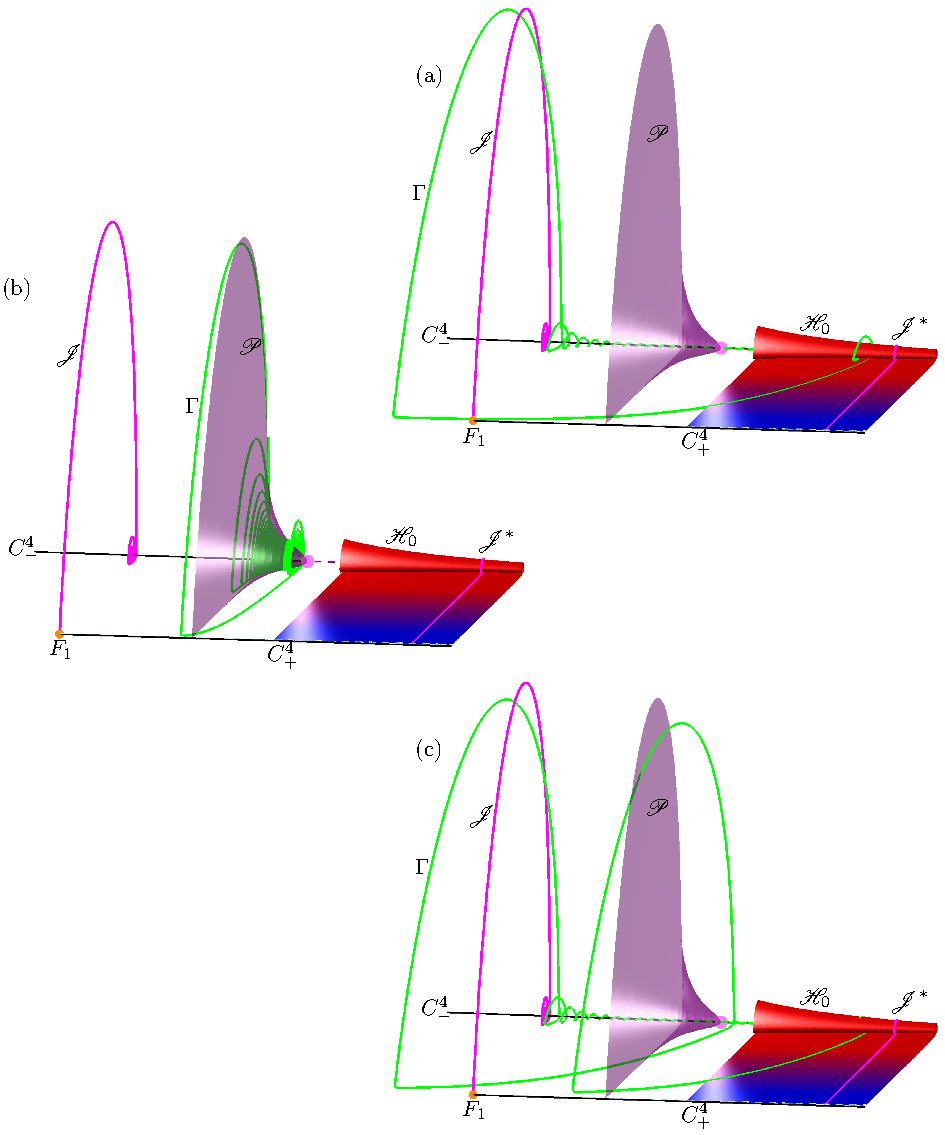
\includegraphics[]{./figures/MKMO_19.pdf}
\caption{Computation of the intersection curve $\mathscr{H}^{\widehat{B}}$ in $\Lambda$ (charcoal surface) for $\widehat{B}=0.75$, shown in projection onto $(B, A, X)$-space.  Row~(a) shows the pairs $(\mathbf{w},\mathbf{u})$ used to compute the upper part of $\mathscr{H}^{\widehat{B}}$ when $\mathbf{w}$ is entirely to the left of $\Lambda$; and row~(b) shows the pairs $(\mathbf{w},\mathbf{u})$ used to compute the lower part of $\mathscr{H}^{\widehat{B}}$ when $\mathbf{u}$ is entirely to the left of $\Lambda$. Here the surface traced out by $\mathbf{w}$ is red with a sample orbit in forest-green, and the surface traced out by $\mathbf{u}$ is colored blue with a sample orbit in magenta.  Panels~(a1) and~(b1) provide the respective global view and panels~(a2) and~(b2) are enlargements near $\Lambda$.}
\label{figure_19}
\end{figure}
%%%%%%%%%%%%%%%%%%%%%%%%%%%%%%%%%%%%%%%%%%%%%%%%%%%%%%%%%%

The three-dimensional section $\Lambda$ for fixed $\widehat{B}$ is divided into two regions by a two-dimensional surface of points at which the vector field \eqref{equation_1} is tangent to $\Lambda$ in the $B$-direction; this happens when $\frac{dB}{dt} = 0$, that is, when  $X = 1/\widehat{B}  - AY$ according to \eqref{equation_1}.  This surface, called a tangency locus \cite{tangency_locus_paper}, divides the curve $\mathscr{H}^{\widehat{B}}$ into two parts: along one part the flow of \eqref{equation_1} is from left to right (from larger to smaller values of $B$), and along the other the flow is from right to left.  Our algorithm computes both pieces of $\mathscr{H}^{\widehat{B}}$, corresponding to the pieces of $\mathscr{H}$, shown in Figure~\ref{figure_19}, in a single run; see also~\cite{England}. The two pieces are distinguished by the properties of the paired orbit segments $(\mathbf{w},\mathbf{u})$ that represent orbits on $\mathscr{H}$.  Each panel of Figure~\ref{figure_19} shows one of the two pieces of $\mathscr{H}$ computed for $\widehat{B}=0.75$ with the $\mathbf{w}$-family plotted in red and the $\mathbf{u}$-family plotted in blue.  Panel~(a1) shows a global view of the portion of $\mathscr{H}$ for which the flow moves from left to right through $\mathbf{u}(0) \in \mathscr{H}^{\widehat{B}}$.  Panel~(a2) is an enlargement of the region where $\mathscr{H}$ intersects $\Lambda$.  An example orbit segment is shown in forest green and magenta, and we can see that $\mathbf{u}(0)$ lies in the spiralling region of $\mathscr{H}$. Panel~(b1) shows a global view of the portion of $\mathscr{H}$ for which the flow through $\mathbf{u}(0)$ moves from right to left.  Panel~(b2) is an enlargement of the region where $\mathscr{H}$ intersects $\Lambda$, illustrating with an example orbit segment that $\mathbf{u}(0)$ lies in a non-spiralling region of $\mathscr{H}$.  Note that the orbit segments $\mathbf{u}$ in panels~(a1) and~(a2) have the segments to the right of $\Lambda$ in common with the orbit segments $\mathbf{w}$ in panels~(b1) and~(b2).  The pieces of $\mathscr{H}$ shown in Figure~\ref{figure_19}(a1) and Figure~\ref{figure_19}(b1) do not constitute the entire surface $\mathscr{H}$.  This is due to the strong contraction in backward time near $C^2$, which results in many $(\mathbf{w},\mathbf{u})$-pairs being indistinguishable numerically in terms of the end point $\mathbf{u}(0)$.

%%%%%%%%%%%%%%%%%%%%%%%%%%%%%%%%%%%%%%%%%%%%%%%%%%%%%%%%%%
\begin{figure}[t!]
\centering
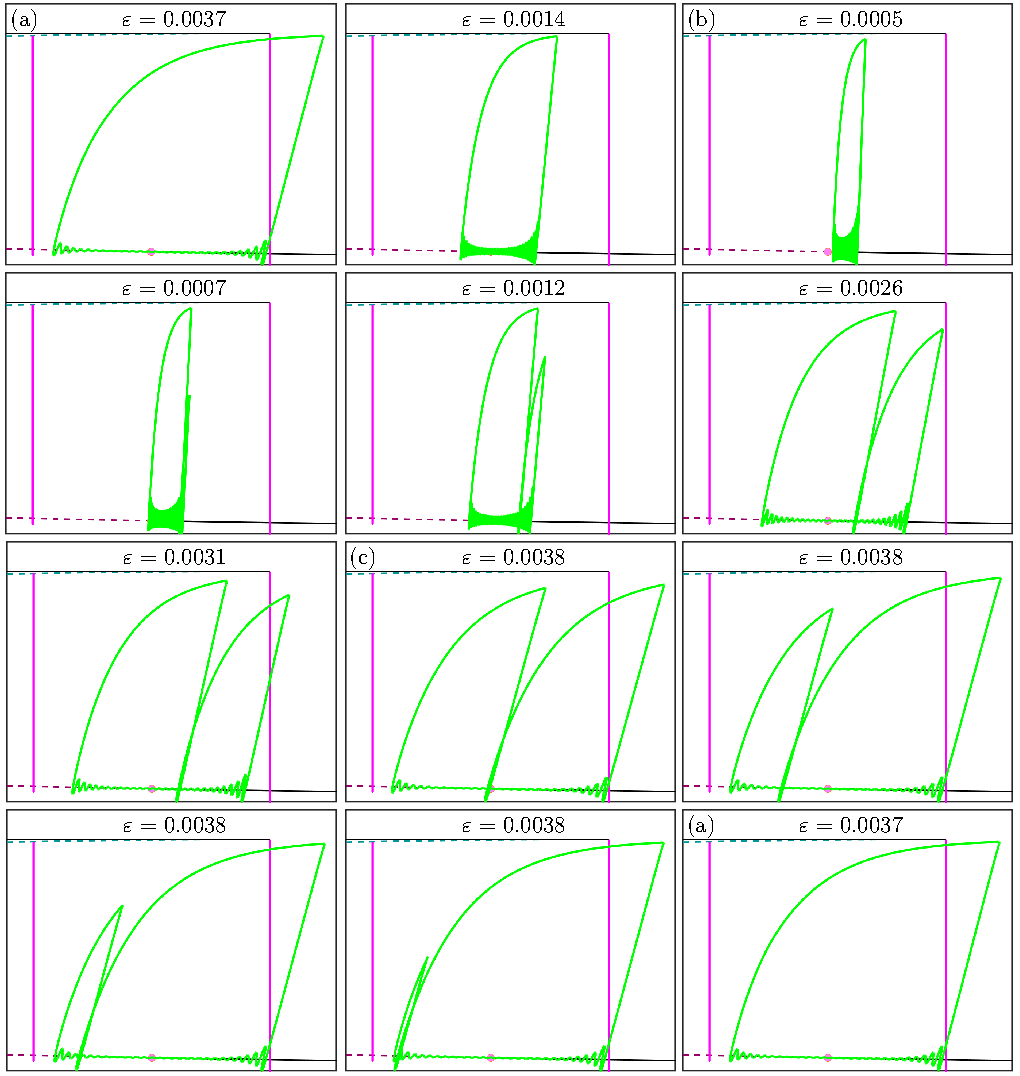
\includegraphics[]{./figures/MKMO_20.pdf}
\caption{Projection onto $(B,A,X)$-space of the intersection curves $\mathscr{H}^{\widehat{B}}$ (royal purple) of $\mathscr{H}$ and $\mathscr{H}_0^{\widehat{B}}$ (green) of $\mathscr{H}_0$ with $\Lambda$ for $\widehat{B}=0.8$, $\widehat{B}=0.75$, $\widehat{B}=0.62$, and $\widehat{B}=0.4$ (left to right).  The curve $\mathscr{H}^{\widehat{B}}$ is visible behind $\mathscr{H}^{\widehat{B}}_0$ only in the region where the curves are spiralling.}
\label{figure_20}
\end{figure}
%%%%%%%%%%%%%%%%%%%%%%%%%%%%%%%%%%%%%%%%%%%%%%%%%%%%%%%%%%

Once computed as described above, we compare $\mathscr{H}_0^{\widehat{B}}$ and $\mathscr{H}^{\widehat{B}}$ inside $\Lambda$ for several choices of $\widehat{B} \in (H_B, F_{1_B})$.  Figure~\ref{figure_20} shows intersection curves $\mathscr{H}_0^{\widehat{B}}$ (green) plotted on top of $\mathscr{H}^{\widehat{B}}$ (purple) for $\widehat{B}=0.8$, $\widehat{B}=0.75$, $\widehat{B}=0.62$, and $\widehat{B}=0.4$ (left to right) in projection onto $(B,A,X)$-space.  Recall that the boundary of $\mathscr{H}^{\widehat{B}}_0$ is $(C^2 \cup C^3) \cap \Lambda$ and the boundary of $\mathscr{H}^{\widehat{B}}$ is $(S^2 \cup S^3) \cap \Lambda$.  Therefore, differences in the boundary points of  $\mathscr{H}^{\widehat{B}}$ and $\mathscr{H}_0^{\widehat{B}}$ are expected, because $S^3$ and $S^2$ lie $O(\varepsilon)$ away from $C^3$ and $C^2$, respectively.  Near $S^3$, the boundary point of $\mathscr{H}_0^{\widehat{B}}$ has a larger $A$-value, and, in the spiralling region near $S^2$, the boundary point of $\mathscr{H}_0^{\widehat{B}}$ has a smaller $A$-value than the boundary points of $\mathscr{H}^{\widehat{B}}$.  The difference between boundary points of $\mathscr{H}^{\widehat{B}}$ and boundary points of $\mathscr{H}_0^{\widehat{B}}$ is visible in Figure~\ref{figure_20} only for $\widehat{B}=0.4$. There is also a noticeable difference between the respective two curves farther away from the boundary points in areas where $\mathscr{H}^{\widehat{B}}_0$ and $\mathscr{H}^{\widehat{B}}$ spiral.  We can see that more spiraling corresponds to a larger distance between the curves; in other words, the difference between $\mathscr{H}^{\widehat{B}}$ and $\mathscr{H}_0^{\widehat{B}}$ is more pronounced for $\widehat{B}$ closer to $H_B$.

It is not straightforward to define and compute a distance function or norm between two general curves in $\mathbb{R}^3$. The approach we take here is to consider how far the curve $\mathscr{H}^{\widehat{B}}$ is from the curve $\mathscr{H}_0^{\widehat{B}}$, which we measure as the integral over points $l$ on the curve $\mathscr{H}_0^{\widehat{B}}$ of distances to corresponding points in $\mathscr{H}^{\widehat{B}}$. (Note that this distance is not reflexive, since the distance of $\mathscr{H}^{\widehat{B}}$ from $\mathscr{H}_0^{\widehat{B}}$ is not the same as the distance of $\mathscr{H}_0^{\widehat{B}}$ from $\mathscr{H}_0^{\widehat{B}}$.) Instead of the integral, we compute a corresponding sum after mesh discretization, to obtain a discretized distance.  To this end, we assign a mesh of size $N$ to $\mathscr{H}_0^{\widehat{B}}$ and index mesh points, denoted by $l_i$, from $1$ to $N$, starting from those closest to $C^3$.  This can be accomplished by fitting a spline $Spl_0$ to the computed data points on $\mathscr{H}_0^{\widehat{B}}$, obtained by continuation with $\textsc{Auto}$.  Desired mesh points can then be computed with $Spl_0$ at desired arclengths along $\mathscr{H}_0^{\widehat{B}}$.  For each $l_i \in \mathscr{H}_0^{\widehat{B}}$, we denote the associated point on $\mathscr{H}^{\widehat{B}}$ by $k_i \in \mathscr{H}^{\widehat{B}}$.  The discretized distance is then the average distance between the point pairs, given as the sum
%
\begin{equation*}
	d_{\widehat{B}} := \frac{1}{N} \sum_{i=1}^{N} \left \lVert l_i - k_i\right \lVert.
	\label{integral_norm}
\end{equation*}
%

A fundamental difficulty in computing such a distance is that for every $l_i$, we need to make a choice of how to find $k_i$.  This is not straightforward because there is no general way of choosing a coordinate system that defines the point $k_i$  uniquely as a continuous function of the position of $l_i$. Given that  $\mathscr{H}^{\widehat{B}}$ is quite close to $\mathscr{H}_0^{\widehat{B}}$, we define $k_i$ as the closest point in the plane  $\mathscr{N}_i$ through $l_i$ that is perpendicular to (the tangent of) $\mathscr{H}^{\widehat{B}}_0$ at $l_i$. Hence, $k_i$ is found as the intersection point in $\mathscr{N}_i \cap \mathscr{H}^{\widehat{B}}$ that is closest to $l_i$. Indeed, a fundamental issue is that in general $\mathscr{N}_i \cap \mathscr{H}^{\widehat{B}}$ may consist of more than one point, or may even be empty. This problem notwithstanding, the $k_i$ can readily be computed for all $l_i$ (if they exist).  

%%%%%%%%%%%%%%%%%%%%%%%%%%%%%%%%%%%%%%%%%%%%%%%%%%%%%%%%%%
\begin{figure}[t!]
\centering
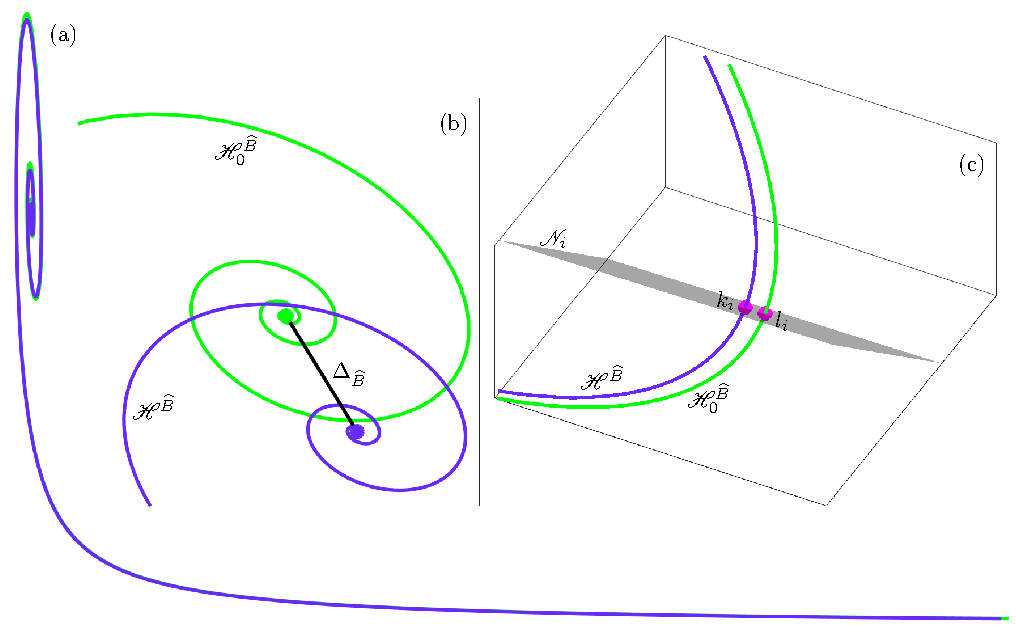
\includegraphics[]{./figures/MKMO_21.pdf}
\caption{Intersection curves $\mathscr{H}^{\widehat{B}}$ (royal purple) and $\mathscr{H}_0^{\widehat{B}}$ (green) for $\widehat{B}=0.75$ projected onto the $(A,X)$-plane (a).  An enlargement of the spiralling region near the end points of the curves is shown in panel~(b) with the line of length $\Delta_{\widehat{B}}$ connecting them.  Panel~(c) shows a further enlargement of the spiralling region inside the section $\Lambda$, represented by  $(A,X,Y)$-space, with the plane $\mathscr{N}_i$ (charcoal surface) that is normal to $\mathscr{H}_0^{\widehat{B}}$ at the point $l_i$ (magenta dot).  The corresponding point $k_i$ on $\mathscr{H}^{\widehat{B}}$ is also shown in magenta.}
\label{figure_21}
\end{figure}
%%%%%%%%%%%%%%%%%%%%%%%%%%%%%%%%%%%%%%%%%%%%%%%%%%%%%%%%%%

Before such a computation can start, one must deal with the problem that one end of one of the two curve `sticks out' beyond the end point of the other curve, so that $l_i$ near the boundary points of $\mathscr{H}_0^{\widehat{B}}$ may not have appropriate matches $k_i$ on $\mathscr{H}^{\widehat{B}}$; see Figure~\ref{figure_20}(a), where $\mathscr{H}_0^{\widehat{B}}$ (green curve) and $\mathscr{H}^{\widehat{B}}$ (purple curve) are shown for $\widehat{B}=0.75$. To avoid this problem, we first truncate $\mathscr{H}_0^{\widehat{B}}$ near $C^3$ so that at its first (mesh) point the plane normal to $\mathscr{H}_0^{\widehat{B}}$ intersects the first computed data point of $\mathscr{H}^{\widehat{B}}$.  At their other end points, the two curves approach $C^3$ and $S^3$, respectively, and we denote by $\Delta_{\widehat{B}}$ the distance between these two computed end points, representing $C^3 \cap \Lambda$ and $S^3 \cap \Lambda$; see Figure~\ref{figure_20}(b), where $\Delta_{\widehat{B}} \approx 0.009796$ is represented by a connecting black line. Near $C^3$, where the curves do not spiral, we truncate $\mathscr{H}_0^{\widehat{B}}$ with a perpendicular plane. However, near $C^2$ this approach is not suitable because $\mathscr{H}_0^{\widehat{B}}$ may spiral into the point $C^2 \cap \Lambda$; instead, we truncate $\mathscr{H}_0^{\widehat{B}}$ so that its last (mesh) point has distance $2\Delta_{\widehat{B}}$ from $C^2 \cap \Lambda$.

With the built in \textsc{Matlab} function \texttt{spline}, we fit splines $Spl_0$ and $Spl$ to the truncated curves $\mathscr{H}_0^{\widehat{B}}$ and $\mathscr{H}^{\widehat{B}}$, respectively.  Apart from the truncated end points, we choose the set of computed data points obtained from the $\textsc{Auto}$ continuation as the mesh points $l_i$ on $\mathscr{H}_0^{\widehat{B}}$, which gives a mesh with well over $N=700$ mesh points. For each $l_i$, we apply the built-in \textsc{Matlab} function \texttt{fnder} to $Spl_0$ to obtain a unit tangent vector, which is then used to define $\mathscr{N}_i$.  The points $k_i \in \mathscr{N}_i$ are then computed with the spline function $Spl$. The enlargement in Figure~\ref{figure_21}(c) shows a representative $(l_i, k_i)$-pair (magenta dots) on $\mathscr{H}_0^{\widehat{B}}$ and $\mathscr{H}^{\widehat{B}}$, respectively, and the corresponding $\mathscr{N}_i$ (charcoal plane). This is the situation, like for most points $l_i$, where there is (locally) a unique intersection point. Indeed, there are generally other intersection points with $\mathscr{N}_i$ much further away when $\mathscr{H}_0^{\widehat{B}}$ and $\mathscr{H}^{\widehat{B}}$  are spiralling, and this if why we choose $k_i$ to be the intersection with the smallest arclength distance from $k_{i-1}$, which is locally consistent. 

The spiralling nature of the two points we are comparing creates certain geometric issues for finding $k_i$. It may happen at some $l_i$ that there is no local intersection (near $k_{i-1}$) between $\mathscr{H}^{\widehat{B}}$ and $\mathscr{N}_i$ any longer (there will generally be other intersection points further away from $l_i$ with other arms of the spiral); this arises when the normal plane to $\mathscr{H}_0^{\widehat{B}}$ becomes tangent to the curve $\mathscr{H}^{\widehat{B}}$ in between the points $l_{i-1}$ and $l_i$. We find that this happens only at only a few points of the mesh, and we omit these mesh points from the calculation of the distance average $d_{\widehat{B}}$ of \eqref{integral_norm}, which means adjusting the mesh size $N$ accordingly. A less serious issue is that segments of $\mathscr{H}^{\widehat{B}}$ may be outside the convolute of $\mathscr{H}_0^{\widehat{B}}$. In this case, local intersection points $k_i$ can still be determined uniquely, but the sequence $(k_i)$ is then no longer ordered by arclength along $\mathscr{H}^{\widehat{B}}$. In particular, this illustrates that the distance we consider is not invariant with respect to exchanging the two curves; that is, the distance $d_{\widehat{B}}$ of $\mathscr{H}^{\widehat{B}}$ from $\mathscr{H}_0^{\widehat{B}}$ that we compute is not the same as the distance of $\mathscr{H}_0^{\widehat{B}}$ from $\mathscr{H}^{\widehat{B}}$ (where the points $l_i$ are on $\mathscr{H}^{\widehat{B}}$). 



%%%%%%%%%%%%%%%%%%%%%%%%%%%%%%%%%%%%%%%%%%%%%%%%%%%%%%%%%%
\begin{table}[t!]
    \tbl{Distances $\Delta_{\widehat{B}}$ between $C^2 \cap \Lambda$ and $S^3 \cap \Lambda$, and $d_{\widehat{B}}$ between $\mathscr{H}_0^{\widehat{B}}$ and $\mathscr{H}^{\widehat{B}}$ for selected values of $\widehat{B}$.}
        {\begin{tabular}{c  c  c  c  c  c  c  c  c} \\[-2pt]
            \toprule
            $\widehat{B}$ & $0.4$ & $0.62$ & $0.75$ & $0.8$  \\[6pt]
            \hline\\[-6pt]
            $\Delta_{\widehat{B}}$ & $1.02414 \times 10^{-3}$ & $10.90585 \times 10^{-3}$ & $9.79563 \times 10^{-3}$ & $6.97168 \times 10^{-3}$ \\[6pt]
            \hline\\[-6pt]
            $d_{\widehat{B}}$ & $0.0460310 \times 10^{-2}$ & $1.47538 \times 10^{-2}$ & $0.763856 \times 10^{-2}$ & $1.109913 \times 10^{-2}$ \\[1pt]
            \botrule
        \end{tabular}}
\label{table:dist}
\end{table}
%%%%%%%%%%%%%%%%%%%%%%%%%%%%%%%%%%%%%%%%%%%%%%%%%%%%%%%%%%

We find that the distance $d_{\widehat{B}}$, computed as explained above for a number of values of $\widehat{B}$, provides a practical measure of how close the suface $\mathscr{H}$ for $\varepsilon = 0.0037$ is from its singular surface $\mathscr{H}_0$. Specifically, we computed the distance for the curves shown in Figure~\ref{figure_20}, and the results are summarized in Table~\ref{table:dist}. Note that the distances $d_{\widehat{B}}$ between the curves $\mathscr{H}_0^{\widehat{B}}$ and $\mathscr{H}^{\widehat{B}}$ are of same order as the distance  $\Delta_{\widehat{B}}$ between their end points $C^2 \cap \Lambda$ and $S^3 \cap \Lambda$. This agrees with the general results \cite{Fenichel} that the distance of $S^3$ from $C^2$ and the distance of $\mathscr{H}$ from $\mathscr{H}_0$ are both of order $O(\varepsilon)$. Note that $\Delta_{\widehat{B}}$ and $d_{\widehat{B}}$ increase with $\widehat{B}$ increases; this is to be expected since $\mathscr{H}_0^{\widehat{B}}$ and $\mathscr{H}^{\widehat{B}}$ are spiralling increasingly the closer $\widehat{B}$ is to the value $B_H$ where the singular Hopf bifurcation occurs.  

Overall, the values of $\Delta_{\widehat{B}}$ and $d_{\widehat{B}}$ in Table~\ref{table:dist} are all at most of order $10^{-2}$, which quantifies the observation from Figure~\ref{figure_13} that the surface $\mathscr{H}$ for $\varepsilon = 0.0037$ and the singular surface $\mathscr{H}_0$ are very close to each other. In fact, sufficiently so to justify studying the $\varepsilon$-dependent MMO periodic orbit $\Gamma$ in Section~\ref{sec:mmogeom} along its isola for $\varepsilon \in [0.00055, 0.00389]$ in relation to the singular objects for $\varepsilon = 0$, which include, in particular, the surface $\mathscr{H}_0$.


%%%%%%%%%%%%%%%%%%%%%%%%%%%%%%%%%%%%%%%%%%%%%%%%%%%%%%%%%%
%%% References

%% \bibliographystyle{ws-ijbc}
%% \bibliography{mko_het_olsen}
%
\begin{thebibliography}{46}
\newcommand{\enquote}[1]{``#1''}
\providecommand{\natexlab}[1]{#1}
\providecommand{\url}[1]{\texttt{#1}}
\providecommand{\urlprefix}{URL }
\expandafter\ifx\csname urlstyle\endcsname\relax
  \providecommand{\doi}[1]{doi:\discretionary{}{}{}#1}\else
  \providecommand{\doi}{doi:\discretionary{}{}{}\begingroup
  \urlstyle{rm}\Url}\fi

\bibitem[{Beno{\^i}t(1982)}]{lents-rapides}
Beno{\^i}t, E. [1982] \enquote{Syst{\`e}mes lents-rapides dans $\mathbb{R}^3$
et leurs canards,} \emph{Proceedings of the Third Schnepfenried Geometry
Conference} \textbf{2},  159--191.
%
%% \bibitem[{Beno{\^i}t(1985)}]{enlacement}
%%  Beno{\^i}t, E. [1985] \enquote{Enlacements de canards,} \emph{Comptes Rendus
%%   Mathematique Academie des Sciences} \textbf{300},  225--230.
%
\bibitem[{Beno{\^i}t \emph{et~al.}(1981)Beno{\^i}t, Callot, Diener \&
Diener}]{canard_explosion}
Beno{\^i}t, E., Callot, J.~F., Diener, F. \& Diener, M. [1981] \enquote{Chasse
au canard,} \emph{Collectanea Mathematica} \textbf{31},  37--119.
% 
\bibitem[{Bertram \emph{et~al.}(1995)Bertram, Butte, Kiemel \& Sherman}]{bertram95}
Bertram, R., Butte, M.~J., Kiemel, T. \& Sherman, A. [1995]
\newblock \enquote{Topological and phenomenological classification of bursting oscillations,}
\newblock \emph{Bulletin of Mathematical Biology} \textbf{57}(3), 413--439.
%
\bibitem[{Bold \emph{et~al.}(2003)Bold, Edwards, Guckenheimer, Guharay, Hoffman, Hubbard, Oliva \& Weckesser}]{vdp2}	
Bold, K., Edwards, C., Guckenheimer, J., Guharay, S., Hoffman, K., Hubbard, J., Oliva, R. \& Weckesser, W. [2003]
\newblock \enquote{The forced van der Pol equation II: Canards in the reduced system,}
\newblock \emph{Journal on Applied Dynamical Systems} \textbf{2}(4), 570--608.
% 
\bibitem[{Br{\o}ns \& Bar-Eli(1991)}]{BZ_reaction}
Br{\o}ns, M. \& Bar-Eli, K. [1991] \enquote{Canard explosion and excitation in
a model of the {B}elousov-{Z}habotinskii reaction,} 
\emph{Journal of Physical Chemistry A} \textbf{95},  8706--8713.
% 
%% \bibitem[{Br{\o}ns \emph{et~al.}(2015)Br{\o}ns, Desroches \&
%%   Krupa}]{Forest_pest_model}
%%  Br{\o}ns, M., Desroches, M. \& Krupa, M. [2015] \enquote{Mixed--mode
%%   oscillations due to a singular hopf bifurcation in a forest pest model,}
%%   \emph{International Journal of Mathematical Demography} \textbf{22},  71--79.
% 
%% \bibitem[{Br{\o}ns \emph{et~al.}(2006)Br{\o}ns, Krupa \&
%%   Wechselberger}]{folded_node}
%%  Br{\o}ns, M., Krupa, M. \& Wechselberger, M. [2006] \enquote{Mixed mode
%%   oscillations due to the generalized canard phenomenon,} \emph{Fields
%%   Institute Communications} ,  39--63.
% 
%% \bibitem[{De~Maesschalck \& Wechselberger(2015)}]{Neurons}
%%  De~Maesschalck, P. \& Wechselberger, M. [2015] \enquote{{Neural Excitability
%%   and Singular Bifurcations}.} \emph{The Journal of Mathematical Neuroscience}
%%   \textbf{5}.
% 
\bibitem[{Desroches \emph{et~al.}(2012)Desroches, Guckenheimer, Krauskopf, Kuehn, Osinga \& Wechselberger}]{MMO}
Desroches, M., Guckenheimer, J., Krauskopf, B., Kuehn, C., Osinga, H.~M. \& Wechselberger, M. [2012]
\newblock \enquote{{Mixed-mode oscillations with multiple time scales}.}
\newblock \emph{SIAM Review} \textbf{54}(2), 211--288.
% 
\bibitem[{Desroches \emph{et~al.}(2009)Desroches, Krauskopf \& Osinga}]{QSSA}
Desroches, M., Krauskopf, B. \& Osinga, H. [2009]
\newblock \enquote{{The geometry of mixed-mode oscillations in the {O}lsen model for peroxidase-oxidase reaction}.}
\newblock \emph{Discrete \& Continuous Dynamical Systems} \textbf{2}(4), 807--827.
% 
\bibitem[{Desroches \emph{et~al.}(2008)Desroches, Krauskopf \& Osinga}]{homotopy_example}
Desroches, M., Krauskopf, B. \& Osinga, H.~M. [2008]
\newblock \enquote{Mixed-mode oscillations and slow manifolds in the self-coupled {F}itz{H}ugh--{N}agumo system,}
\newblock \emph{Chaos} \textbf{18}(1), 015107.
% 
\bibitem[{Desroches \emph{et~al.}(2010)Desroches, Krauskopf \& Osinga}]{Nonlinearity}
Desroches, M., Krauskopf, B. \& Osinga, H.~M. [2010]
\newblock \enquote{Numerical continuation of canard orbits in slow-fast dynamical systems,}
\newblock \emph{Nonlinearity} \textbf{23}(3),  739--765.
%
\bibitem[{Doedel(1981)}]{autoOriginal}
Doedel, E.~J. [2007]
\newblock \enquote{{AUTO}, a program for the automatic bifurcation analysis of autonomous systems,}
\newblock {\em Congressus Numerantium} \textbf{30}, 265--384.
%
\bibitem[{Doedel \& Oldeman(2007)}]{auto}
Doedel, E.~J. \& Oldeman, B. [2007]
\newblock \emph{AUTO-07p: Continuation and bifurcation software for ordinary differential equations},
\newblock available at\urlprefix\url{http://indy.cs.concordia.ca/auto/}; with major contributions
  from Champneys, A.~R., Dercole, F., Fairgrieve, T.~F., Kuznetsov, Yu.~A., Paffenroth, R.~C., Sandstede, B., Wang, X. \& Zhang, C.
%
\bibitem[{England \emph{et~al.}(2005)England, Krauskopf \& Osinga}]{England}
England, J.~P., Krauskopf, B. \& Osinga, H.~M. [2005]
\newblock \enquote{Computing one-dimensional global manifolds of {P}oincar{\'e} maps by continuation,}
\newblock \emph{Journal on Applied Dynamical Systems} \textbf{4}(4), 1008--1041.
%
\bibitem[{Farjami \emph{et~al.}(2018)Farjami, Kirk \& Osinga}]{Saeed_Paper}
Farjami, S., Kirk, V. \& Osinga, H.~M. [2018]
\newblock \enquote{{Computing the stable manifold of a saddle slow manifold}.}
\newblock \emph{SIAM Journal on Applied Dynamical Systems} \textbf{17}(1),  350--379.
%
\bibitem[{Fenichel(1979)}]{Fenichel}
Fenichel, N. [1979]
\newblock \enquote{Geometric singular perturbation theory for ordinary differential equations,}
\newblock \emph{Journal of Differential Equations} \textbf{31}(1),  53--98.
%
\bibitem[{FitzHugh(1955)}]{FH}
FitzHugh, R. [1955] \enquote{Mathematical models of threshold phenomena in the
nerve membrane,} \emph{The bulletin of Mathematical Biophysics} \textbf{17}(4), 257--278.
% 
%% \bibitem[{Guckenheimer(2008)}]{singular_hopf}
%%  Guckenheimer, J. [2008] \enquote{Singular hopf bifurcation in systems with two
%%   slow variables,} \emph{SIAM Journal on Applied Dynamical Systems} \textbf{7}(4),
%%    1355--1377.
%
\bibitem[{Guckenheimer \emph{et~al.}(2003)Guckenheimer, Hoffman \& Weckesser}]{vdp1}
Guckenheimer, J., Hoffman, K. \& Weckesser, W. [2003]
\newblock \enquote{The forced van der Pol equation I: The slow flow and its bifurcations,}
\newblock \emph{SIAM Journal on Applied Dynamical Systems} \textbf{2}(1), 1--35.
%
\bibitem[{Guckenheimer \& Holmes(1986)}]{GH}
Guckenheimer, J. \& Holmes, P. [1986]
\newblock \emph{Nonlinear Oscillations, Dynamical Systems and Bifurcations of Vector Fields}, 2nd Ed.
\newblock (Springer-Verlag, New York).
%
\bibitem[{Guckenheimer \& Kuehn(2009)}]{gk-siads09}
Guckenheimer, J. \& Kuehn, C. [2009]
\newblock \enquote{Computing slow manifolds of saddle type,}
\newblock \emph{SIAM Journal on Applied Dynamical Systems} \textbf{8}(3), 854--879.
% 
%% \bibitem[{H{\'a}ro \& de~la Llave(2006)}]{Invariant_tori_again}
%%  H{\'a}ro, A. \& de~la Llave, R. [2006] \enquote{A parameterization method for
%%   the computation of invariant tori and their whiskers in quasi-periodic maps:
%%   Rigorous results,} \emph{Journal of Differential Equations} \textbf{228},
%%   530--579.
% 
\bibitem[{Harvey \emph{et~al.}(2010)Harvey, Kirk, Osinga, Sneyd \& Wechselberger}]{Emily_Harvey_paper}
Harvey, E., Kirk, V., Osinga, H.~M., Sneyd, J. \& Wechselberger, M. [2010]
\newblock \enquote{Understanding anomalous delays in a model of intracellular calcium dynamics,}
\newblock \emph{Chaos} \textbf{20}(4), 045104.
% 
\bibitem[{Hasan \emph{et~al.}(2018)Hasan, Krauskopf \& Osinga}]{Cris_paper}
Hasan, C., Krauskopf, B. \& Osinga, H.~M. [2018]
\newblock \enquote{Saddle slow manifolds and canard orbits in {$\mathbb{R}^4$} 
and application to the full {H}odgkin--{H}uxley model,}
\newblock \emph{Journal of Mathematical Neuroscience} \textbf{8}, 5.
% 
\bibitem[{Hodgkin \& Huxley(1952)}]{HH}
Hodgkin, A.~L., Huxley A.~F. [1952] 
\newblock \enquote{A quantitative description of membrane 
current and its application to conduction and excitation in nerve,}
\newblock \emph{Journal of Physiology} \textbf{117}(4), 500--544.
% 
\bibitem[{Hudson \emph{et~al.}(1979)Hudson, Hart \& Marinko}]{BZ}
Hudson, J.~L., Hart, M. \& Marinko, D. [1979] \enquote{An experimental study of
multiple peak periodic and nonperiodic oscillations in the
{B}elousov-{Z}habotinskii reaction,} \emph{The Journal of Chemical Physics}
\textbf{71},  1601--1606.
% 
\bibitem[{Izhikevich(2000)}]{izh00}
Izhikevich, E. M. [2000]
\newblock \enquote{Neural excitability, spiking and bursting,}
\newblock \emph{Intl. J. Bifurcation \& Chaos} \textbf{10}(6), 1171--1266.
% 
%% \bibitem[{Jorba \& Olmedo(2009)}]{Invariant_tori}
%%  Jorba, A. \& Olmedo, E. [2009] \enquote{On the computation of reducible
%%   invariant tori on a parallel computer,} \emph{SIAM Journal on Applied
%%   Mathematics} \textbf{8},  1382--1404.
% 
\bibitem[{Jones(1995)}]{Jones}
Jones, C.~K.~R.~T. [1995]
\newblock \enquote{Geometric singular perturbation theory,} 
\newblock Lecture Notes in Mathematics, vol. 1609,
(Springer-Verlag, New York), pp. 44--118.
%
\bibitem[{Krauskopf \& Osinga(2007)}]{Red_book}
Krauskopf, B. \& Osinga, H.~M. [2007]
\newblock \enquote{Computing invariant manifolds via the continuation of orbit segments,}
\newblock \emph{Numerical Continuation Methods for Dynamical Systems}, eds. Krauskopf, B., Osinga, H.~M. \&
  Gal{\'a}n-Vioque, J. (Springer-Verlag, New York), Chapter 4, pp. 117--154.
%
\bibitem[{Krauskopf \& Rie{\ss}(2008)}]{Lin_POs}
Krauskopf, B. \& Rie{\ss}, T. [2008]
\newblock \enquote{{A {L}in's method approach to finding and continuing heteroclinic connections involving periodic orbits}.}
\newblock \emph{Nonlinearity} \textbf{21}(8),  1655--1690.
%
%% \bibitem[{Krupa \emph{et~al.}(2008)Krupa, Popovi{\'c} \& Kopell}]{three}
%%  Krupa, M., Popovi{\'c}, N. \& Kopell, N. [2008] \enquote{Mixed-mode
%%   oscillations in three time-scale systems: A prototypical example,} \emph{SIAM
%%   Journal on Applied Dynamical Systems} ,  361--420.
% 
\bibitem[{Kuehn \& Szmolyan(2015)}]{Rescaling}
Kuehn, C. \& Szmolyan, P. [2015]
\newblock \enquote{{Multiscale geometry of the {O}lsen model and non-classical relaxation oscillations}.} \newblock \emph{Journal of Nonlinear Science} \textbf{25}(3),  583--629.
% 
\bibitem[{Kuznetsov(1998)}]{The_Kuz}
Kuznetsov, Y.~A. [1998]
\newblock \emph{Elements of Applied Bifurcation Theory}, 2nd Ed.
\newblock (Springer-Verlag, New York).
% 
\bibitem[{Nagumo \& Arimoto(1962)}]{Nagumo}
Nagumo J.~S. \& Arimoto, S. [1962]
\newblock \emph{An active pulse transmission line simulating nerve axon,} 
\newblock \emph{Proceedings of IRE 1962} \textbf{50}(10), 2061--2070.
%
\bibitem[{Lee \emph{et~al.}(2008)Lee, Collins, Krauskopf \& Osinga}]{tangency_locus_paper}
Lee, C.~M., Collins, P.~J., Krauskopf, B. \& Osinga, H.~M. [2008]
\newblock \enquote{Tangency bifurcations of global {P}oincar{\'e} maps,}
\newblock \emph{SIAM Journal of Applied Dynamical Systems} \textbf{7}(3),  712--754.
% 
\bibitem[{Lin(1989)}]{Lin_original}
Lin, X. [1989]
\newblock \enquote{Shadowing lemma and singularly perturbed boundary value problems,}
\newblock \emph{SIAM Journal of Applied Mathematics} \textbf{49}(1),  26--54.
%
\bibitem[{Lizarraga \& Wechselberger(2019)}]{Lizarraga_paper}
Lizarraga, I. \& Wechselberger, M. [2019]
\newblock \enquote{Computational singular perturbation method for nonstandard slow-fast systems,}
\newblock {a}rXiv:1906.06049.
%
%% \bibitem[{Milik(1998)}]{Rescaling_earlier_work}
%%  Milik, A. [1998] \enquote{Mixed-mode oscillations in chemical systems,}  PhD
%%   thesis, Vienna University of Technology.
% 
\bibitem[{Milik \emph{et~al.}(1998)Milik, Szmolyan, L{\"o}ffelmann \& Gr{\"o}ller}]{Autocatalator}
Milik, A., Szmolyan, P., L{\"o}ffelmann, H. \& Gr{\"o}ller, E. [1998]
\newblock \enquote{Geometry of mixed-mode oscillations in the 3--d autocatalator,}
\newblock \emph{International Journal of Bifurcation and Chaos} \textbf{8}(3),  505--519.
%
%% \bibitem[{Mitry \emph{et~al.}(2013)Mitry, McCarthy, Kopell \&
%%   Wechselberger}]{Martin_neuron_paper}
%%  Mitry, J., McCarthy, M., Kopell, N. \& Wechselberger, M. [2013]
%%   \enquote{Excitable neurons, firing threshold manifolds and canards,}
%%   \emph{The journal of mathematical neuroscience} \textbf{3}.
% 
\bibitem[{Mujica \emph{et~al.}(2017)Mujica, Krauskopf \& Osinga}]{Jose_Paper}
Mujica, J., Krauskopf, B. \& Osinga, H.~M. [2017]
\newblock \enquote{{A {L}in's method approach for detecting canard orbits near a folded node}.}
\newblock \emph{Journal of Computational Dynamics} \textbf{4}(1),  143--165.
%
\bibitem[{Nowacki \emph{et~al.}(2012)Nowacki, Osinga \& Tsaneva-Atanasova}]{nota-jmn}
Nowacki, J., Osinga, H.~M. \& Tsaneva-Atanasova , K.~T. [2012]
\newblock \enquote{Dynamical systems analysis of spike-adding mechanisms in transient bursts,}
\newblock \emph{The Journal of Mathematical Neuroscience} \textbf{2}, 7.
%
\bibitem[{Olsen(1983)}]{Olsen}
Olsen, L. [1983]
\newblock \enquote{An enzyme reaction with a strange attractor,}
\newblock \emph{Physics Letters A} \textbf{94}(9), 454--457.
%
\bibitem[{Osinga \emph{et~al.}(2012)Osinga, Sherman \& Tsaneva-Atanasova}]{osta-dcds}
Osinga, H.~M., Sherman, A. \& Tsaneva-Atanasova, K.~T. [2012]
\newblock \enquote{Cross-currents between biology and mathematics: The codimension of pseudo-plateau bursting,}
\newblock \emph{Discrete and Continuous Dynamical Systems -- Series A} \textbf{32}(8), 2853--2877.
%
%%  \bibitem[{Otto \emph{et~al.}(2012)Otto, L{\"u}dge, Vladimirov, Wolfrum \&
%%    Sch{\"o}ll}]{lasers}
%%   Otto, C., L{\"u}dge, K., Vladimirov, A.~G., Wolfrum, M. \& Sch{\"o}ll, E.
%%    [2012] \enquote{Delay-induced dynamics and jitter reduction of passively
%%    mode-locked semiconductor lasers subject to optical feedback,} \emph{New
%%    Journal of Physics} \textbf{14}.
%
\bibitem[{Palis \& de Melo(1982)}]{PdM}
Palis, J. \& de~Melo, W. [1982]
\newblock \emph{Geometric Theory of Dynamical Systems}.
\newblock (Springer-Verlag, New York).
%
\bibitem[{Perko(2001)}]{Perko_book}
Perko, L. [2001] \emph{Differential Equations and Dynamical Systems}, 3rd Ed.
  (Springer International Publishing).
%
%% \bibitem[{Piltz \emph{et~al.}(2017)Piltz, Veerman, Maini \&
%%   Porter}]{Predator-Prey}
%%  Piltz, S.~H., Veerman, F., Maini, P.~K. \& Porter, M.~A. [2017] \enquote{A
%%   predator–2 prey fast–slow dynamical system for rapid predator evolution,}
%%   \emph{SIAM Journal on Applied Dynamical Systems} \textbf{16},  54--90.
% 
\bibitem[{Rinzel(1987)}]{rinzel87} 
Rinzel, J. [1987]
\newblock \enquote{A formal classification of bursting mechanisms in excitable systems,}
\newblock \emph{Proc. International Congress of Mathematicians, Berkeley 1986}, ed. Gleason, A.~M. Vol.~2,  pp.~1578--1593.
\newblock (American Mathematical Society, Providence RI);
\newblock also [1987] \emph{Mathematical Topics in Population Biology, Morphogenesis and Neuroscience}, eds. Teramoto, E. \& Yamaguti, M. Lecture Notes in Biomathematics \textbf{71} (Springer-Verlag, Berlin), pp.~267--281 (with slight differences).
%
\bibitem[{Rockafellar \& Wets(2009)}]{Hausdorff_Distance}
Rockafellar, R.~T. \& Wets, R. J.-B. [2009]
\newblock \emph{Variational Analysis}, 3rd Ed.
\newblock (Springer International Publishing).
%
\bibitem[{Stern \emph{et~al.}(2008)Stern, Osinga, Lebeau \& Sherman}]{sols-bmb}
Stern, J.~V., Osinga, H.~M., LeBeau, A. \& Sherman, A. [2008]
\newblock \enquote{Resetting behavior in a model of bursting in secretory pituitary cells: Distinguishing plateaus from pseudo-plateaus,}
\newblock \emph{Bulletin of Mathematical Biology} \textbf{70}(1), 68--88.
%
\bibitem[{Szmolyan \& Wechselberger(2001)}]{SW}
Szmolyan, P. \& Wechselberger, M. [2001]
\newblock \enquote{Canards in $\mathbb{R}^3$,}
\newblock {\em Journal of Differential Equations}, 177(2), 419--453.
%
\bibitem[{Van~der Pol(1926)}]{vdpol}
Van der Pol, B. [1926]
\newblock \enquote{On `relaxation oscillations',}
\newblock \emph{The London, Edinburgh, and Dublin Philosophical Magazine and Journal of Science 
Series 7}, 2(11), 978-–992.
%
%% \bibitem[{Van~der Pol(1927)}]{Circuits}
%%  Van der Pol, B. [1927] \enquote{Forced oscillations in a circuit with 
%%   non-linear resistance. (reception with reactive triode),} \emph{The London,
%%   Edinburgh, and Dublin Philosophical Magazine and Journal of Science}
%%   \textbf{3},  65--80.
% 
\bibitem[{Vo \emph{et~al.}(2013)Vo, Bertram \& Wechselberger}]{Vo_paper}
Vo, T., Bertram, R. \& Wechselberger, M. [2013]
\newblock \enquote{Multiple geometric viewpoints of mixed mode dynamics associated with pseudo-plateau
  bursting,}
\newblock \emph{SIAM Journal on Applied Dynamical Systems} \textbf{12}(2), 789--830.
%
%%  \bibitem[{Vo \emph{et~al.}(2013{\natexlab{b}})Vo, Tabak, Bertram \&
%%    Wechselberger}]{Vo_paper2}
%%   Vo, T., Tabak, J., Bertram, R. \& Wechselberger, M. [2013{\natexlab{b}}]
%%    \enquote{A geometric understanding of how fast activating potassium channels
%%    promote bursting in pituitary cells,} \emph{Journal of Computational
%%    Neuroscience} \textbf{36}.
%  
%%  \bibitem[{Waalkens \emph{et~al.}(2005)Waalkens, Burbanks \&
%%    Wiggins}]{Initial_conditions_volume}
%%   Waalkens, H., Burbanks, A. \& Wiggins, S. [2005] \enquote{A formula to compute
%%    the microcanonical volume of reactive initial conditions in transition state
%%    theory,} \emph{Journal of Physics A: Mathematical and General} \textbf{38},
%%    L759--L768, \urlprefix\url{http://stacks.iop.org/0305-4470/38/i=45/a=L03}.
%  
\bibitem[{Wechselberger(2005)}]{Wech2005}
Wechselberger, M. [2005]
\newblock \enquote{Existence and bifurcation of canards in $\mathbb{R}^3$ in the case of a folded node,}
\newblock \emph{SIAM Journal on Applied Dynamical Systems} \textbf{4}(1):101--139.
%
\bibitem[{Wechselberger(2020)}]{Wechselberger_book}
Wechselberger, M. [2020]
\newblock \emph{Geometric singular perturbation theory beyond the standard form},
\newblock Frontiers in Applied Dynamics: Reviews and Tutorials (Springer International Publishing).
%
\bibitem[{Zhang \emph{et~al.}(2012)Zhang, Krauskopf \& Kirk}]{Lin_POs2}
Zhang, W., Krauskopf, B. \& Kirk, V. [2012]
\newblock \enquote{How to find a codimension-one heteroclinic cycle between two periodic orbits,}
\newblock \emph{Discrete and Continuous Dynamical Systems -- Series A} \textbf{32}(8), 2825--2851.

\end{thebibliography}

\end{document}

%%%%%%%%%%%%%%%%%%%%%%%%%%%%%%%%%%%%%%%%%%%%%%%%%%%%%%%%%%
%%%%%%%%%%%%%%%%%%%%%%%%%%%%%%%%%%%%%%%%%%%%%%%%%%%%%%%%%%
%%%%%%%%%%%%%%%%%%%%%%%%%%%%%%%%%%%%%%%%%%%%%%%%%%%%%%%%%%
